\documentclass[fleqn,10pt]{wlscirep}
%DIF LATEXDIFF DIFFERENCE FILE
%DIF DEL main_reviewed_version.tex   Sun Oct 18 00:22:07 2026
%DIF ADD main.tex                    Sun Oct 18 00:22:07 2026
\usepackage[utf8]{inputenc}
\usepackage[T1]{fontenc}
\usepackage{multirow}
\usepackage{tabularx}
%DIF 6a6
\usepackage{booktabs} %DIF > 
%DIF -------
\usepackage{float}
\usepackage{algorithm}
\usepackage{algorithmic}
%DIF 9a10-12
\usepackage{amsthm} %DIF > 
\usepackage{xcolor} %DIF > 
\usepackage{url} %DIF > 
%DIF -------
\captionsetup{font=small,labelfont={bf,rm},textfont=rm,justification=justified}
%DIF 10a14
\newtheorem{proposition}{Proposition} %DIF > 
%DIF -------

\renewcommand{\topfraction}{0.9}
\renewcommand{\bottomfraction}{0.8}
\renewcommand{\textfraction}{0.07}
\renewcommand{\floatpagefraction}{0.8}
\renewcommand{\dbltopfraction}{0.9}
\renewcommand{\dblfloatpagefraction}{0.8}
\setcounter{topnumber}{3}
\setcounter{bottomnumber}{2}
\setcounter{totalnumber}{4}
\setcounter{dbltopnumber}{3}

%DIF 22a27-32
\newcommand{\Ltr}{\mathcal{L}^{\mathrm{tr}}} %DIF > 
\newcommand{\Lcv}{\mathcal{L}^{\mathrm{cv}}} %DIF > 
\newcommand{\Lte}{\mathcal{L}^{\mathrm{te}}} %DIF > 
\newcommand{\OGR}{\mathrm{OGR}} %DIF > 
\newcommand{\pmm}{$\pm$} %DIF > 
 %DIF > 
%DIF -------
\title{OGR-Driven Dynamic Loss Balancing for Mitigating Gradient Starvation}

\author[1]{Lakshya}
\author[1,*]{Amit Kumar Bairwa}
\author[1,*]{Varun Tiwari}
\affil[1]{Department of Artificial Intelligence and Machine Learning, School of Computer Science and Engineering, Manipal University Jaipur, Jaipur--Ajmer Express Highway, Jaipur, India.}

\affil[*]{amitkumar.bairwa@jaipur.manipal.edu}
\affil[*]{varun.tiwari@jaipur.manipal.edu}
\affil[*]{Corresponding Authors}

\begin{abstract}
%DIF 34c45
%DIF < Multi modal learning systems are likely to be stuck in one of such traps and it is known as the Modality Laziness trap whereby they over-respond to the best signal in most instances which happens to be the best signal. Visual signal and ignore the weak signals such as the Audio or Text signal. The unified models are their possible limited by this optimization bias. Although fixes such as Gradient Blending or OGM-GE currently exist with most of them being based on expensive pre-computations or noisy and unstable noise. Insertion which is incapable of following the dynamics of training. In this paper, the Modality is presented. Fairness Controller (MFC), a simple and easy to use solution. The idea behind the MFC is to look at the Overfitting-to-Generalization Ratio (OGR) of each modality and dynamically vary the level to which each modality affects the learning process. We were able to test on a controlled synthetic benchmark, and a real-world CREMA-D emotion recognition (7,442 mel spectrogram samples, 6 classes). MFC-A also reduces the difference in modality imbalance by 38.4\% at synthetic benchmark and it also enhances the gap. robustness by $+4.7\%$ at $\sigma{=}0.5$ and $+2.3\%$ at $\sigma{=}1.0$ noise. At actual CREMA-D data the MFC-A is as well as accurate as at the baseline and diminishes the OGR dispersion by 38.9 percent without incurring any overhead of noise injection.At 1024-dim model capacity, MFC-A yields a +3.1\% accuracy gain over the baseline, confirming its value grows with model size.
%DIF -------
Jointly trained multimodal networks tend to rely on whichever modality is easiest to fit and leave the other encoders under-trained, a failure known as modality laziness or gradient starvation. We study a simple, generalization-aware remedy. First, we define the Overfitting-to-Generalization Ratio (OGR), the ratio of a modality's held-out loss to its training loss, as a scale-invariant per-modality diagnostic. Second, we propose MFC-A, a closed-loop controller that gives each unimodal auxiliary loss a weight proportional to a power of its inverse smoothed OGR, so that a modality that starts to memorise is throttled and the others are amplified within a fixed weight budget. MFC-A runs inside a single training run and needs no auxiliary networks, gradient surgery or noise injection. We compare it with five baselines under one protocol (ten paired seeds; disjoint training, controller, tuning and test splits; paired significance tests) on two real audio--video benchmarks, AVE and CREMA-D (actor-disjoint), complemented by a controlled synthetic benchmark and a two-view control. On AVE, MFC-A maintains accuracy (80.2 vs.\ 79.9\%) while reducing the OGR gap by 63\% ($p{=}0.03$) and improving robustness to visual noise, blur and low light ($p<0.04$). On the synthetic benchmark it maintains accuracy while reducing the gap by 41\% ($p<0.001$). On CREMA-D, whose dominant modality is audio, it identifies the overfitting video stream correctly and maintains accuracy, but its gains are not significant. Confidence-based gradient modulation (OGM-GE) on AVE and offline Gradient Blending on CREMA-D achieve larger gains at the cost of a tuned hyper-parameter or an extra probe run. The controller's arithmetic is negligible; its monitoring passes add 2--18\% wall-clock time. %DIF > 
%DIF -------
\end{abstract}
%DIF PREAMBLE EXTENSION ADDED BY LATEXDIFF
%DIF UNDERLINE PREAMBLE %DIF PREAMBLE
\RequirePackage[normalem]{ulem} %DIF PREAMBLE
\RequirePackage{color}\definecolor{RED}{rgb}{1,0,0}\definecolor{BLUE}{rgb}{0,0,1} %DIF PREAMBLE
\providecommand{\DIFadd}[1]{{\protect\color{blue}\uwave{#1}}} %DIF PREAMBLE
\providecommand{\DIFdel}[1]{{\protect\color{red}\sout{#1}}} %DIF PREAMBLE
%DIF SAFE PREAMBLE %DIF PREAMBLE
\providecommand{\DIFaddbegin}{} %DIF PREAMBLE
\providecommand{\DIFaddend}{} %DIF PREAMBLE
\providecommand{\DIFdelbegin}{} %DIF PREAMBLE
\providecommand{\DIFdelend}{} %DIF PREAMBLE
\providecommand{\DIFmodbegin}{} %DIF PREAMBLE
\providecommand{\DIFmodend}{} %DIF PREAMBLE
%DIF FLOATSAFE PREAMBLE %DIF PREAMBLE
\providecommand{\DIFaddFL}[1]{\DIFadd{#1}} %DIF PREAMBLE
\providecommand{\DIFdelFL}[1]{\DIFdel{#1}} %DIF PREAMBLE
\providecommand{\DIFaddbeginFL}{} %DIF PREAMBLE
\providecommand{\DIFaddendFL}{} %DIF PREAMBLE
\providecommand{\DIFdelbeginFL}{} %DIF PREAMBLE
\providecommand{\DIFdelendFL}{} %DIF PREAMBLE
%DIF COLORLISTINGS PREAMBLE %DIF PREAMBLE
\RequirePackage{listings} %DIF PREAMBLE
\RequirePackage{color} %DIF PREAMBLE
\lstdefinelanguage{DIFcode}{ %DIF PREAMBLE
%DIF DIFCODE_UNDERLINE %DIF PREAMBLE
  moredelim=[il][\color{red}\sout]{\%DIF\ <\ }, %DIF PREAMBLE
  moredelim=[il][\color{blue}\uwave]{\%DIF\ >\ } %DIF PREAMBLE
} %DIF PREAMBLE
\lstdefinestyle{DIFverbatimstyle}{ %DIF PREAMBLE
	language=DIFcode, %DIF PREAMBLE
	basicstyle=\ttfamily, %DIF PREAMBLE
	columns=fullflexible, %DIF PREAMBLE
	keepspaces=true %DIF PREAMBLE
} %DIF PREAMBLE
\lstnewenvironment{DIFverbatim}{\lstset{style=DIFverbatimstyle}}{} %DIF PREAMBLE
\lstnewenvironment{DIFverbatim*}{\lstset{style=DIFverbatimstyle,showspaces=true}}{} %DIF PREAMBLE
\lstset{extendedchars=\true,inputencoding=utf8}

%DIF END PREAMBLE EXTENSION ADDED BY LATEXDIFF

\begin{document}

\flushbottom
\maketitle
\thispagestyle{empty}

\noindent\textbf{Keywords:} \DIFdelbegin \DIFdel{Multi-modal Learning, Modality Laziness, Gradient Starvation, Loss Balancing}\DIFdelend \DIFaddbegin \DIFadd{Multimodal learning, Modality imbalance, Gradient starvation, Dynamic loss balancing}\DIFaddend , Overfitting-to-Generalization Ratio (OGR), \DIFdelbegin \DIFdel{Emotion Recognition, Dynamic Modulation, Modality Fairness Controller (MFC)}\DIFdelend \DIFaddbegin \DIFadd{Audio--visual emotion recognition}\DIFaddend .

\DIFdelbegin \section{\DIFdel{Introduction}}
%DIFAUXCMD
\addtocounter{section}{-1}%DIFAUXCMD
\DIFdel{The world is tasted in the colourful mixture of impressions. This is what ideally Proposed AI models should do. Nevertheless, such multimodal architectures are usually difficult to train, and powerful ones like Unified Transformers \mbox{%DIFAUXCMD
\cite{zhang2023meta}}\hskip0pt%DIFAUXCMD
, Image Bind \mbox{%DIFAUXCMD
\cite{girdhar2023imagebind}}\hskip0pt%DIFAUXCMD
, CLIP\mbox{%DIFAUXCMD
\cite{radford2021learning}}\hskip0pt%DIFAUXCMD
and Flamingo\mbox{%DIFAUXCMD
\cite{alayrac2022flamingo}}\hskip0pt%DIFAUXCMD
these become lazy. When one of the modalities (say an image) }\DIFdelend \DIFaddbegin \section*{\DIFadd{Introduction}}
\DIFadd{Multimodal models combine complementary signals, such as images, audio and text, and large unified architectures including CLIP\mbox{%DIFAUXCMD
\cite{radford2021learning}}\hskip0pt%DIFAUXCMD
, Flamingo\mbox{%DIFAUXCMD
\cite{alayrac2022flamingo}}\hskip0pt%DIFAUXCMD
, ImageBind\mbox{%DIFAUXCMD
\cite{girdhar2023imagebind} }\hskip0pt%DIFAUXCMD
and Meta-Transformer\mbox{%DIFAUXCMD
\cite{zhang2023meta} }\hskip0pt%DIFAUXCMD
have made this the default design for perception systems. Training such models jointly is nevertheless fragile. When one modality }\DIFaddend is easier to \DIFdelbegin \DIFdel{learn than }\DIFdelend \DIFaddbegin \DIFadd{fit than another, gradient descent reduces the joint loss mainly through the easier modality, and }\DIFaddend the \DIFdelbegin \DIFdel{other (say audio) then the model neglects the more difficult task. This will be called a Modality Laziness or Gradient Starvation \mbox{%DIFAUXCMD
\cite{pezeshki2021gradient}}\hskip0pt%DIFAUXCMD
. The visual features too are generally means puny and arranged; this presents a simple access point leading to the optimizer. Noisey audio or text may be less or excessive. This means that the high visual gradients would tend to absorb the common weights in the model at almost full costs and the other modalities are under-developed. In the real world such as an autonomous car that may have to hear a siren that it cannot see this blindness can be hazardous. Although the various fixes have been enumerated in various recent surveys, like the Balance Benchmark \mbox{%DIFAUXCMD
\cite{xu2025balancebenchmark}}\hskip0pt%DIFAUXCMD
, most of them are burdensome. Others must be taught a high number of models to get appropriate weights orsimply strive to resolve the problem by introducing random noise, again a common hit-or-miss method, like OGM-GE \mbox{%DIFAUXCMD
\cite{peng2022balanced}}\hskip0pt%DIFAUXCMD
. We propose a more idealistic one the Modality Fairness Controller (MFC). Instead of simply slowing down the fast learner, we pose a simple question: Is this modality in fact generalizing or is it simply memorizing? We can take the first step to having each modality pull its own weight with respect to the actual unified representation by taking the cue of limiting Proposed learning rates by the Generalization Gap.}%DIFDELCMD < 

%DIFDELCMD < %%%
\DIFdel{The visual features are also generally small and arranged and this provides a simple pathway to the optimizer \mbox{%DIFAUXCMD
\cite{pezeshki2021gradient}}\hskip0pt%DIFAUXCMD
. Well-conditioned loss surface Vision features dense, spatially coherent, low-noise (e.g. CIFAR-10 \mbox{%DIFAUXCMD
\cite{krizhevsky2009learning}}\hskip0pt%DIFAUXCMD
) features.
Audio characteristics, such as speaker-varying, temporally noisy (e.g., CREMA-D \mbox{%DIFAUXCMD
\cite{cao2014crema}}\hskip0pt%DIFAUXCMD
) create a more rugged and high-variance landscape. Thus, the powerful visual gradients are inclined to attract the shared weights in the model almost entirely and the remaining modalities are under-developed. The implications cannot be seen in normal assessment but are disastrous when stressed modality. The baseline performance of 83.3\% accuracyfalls to 48.2\% accuracy with the addition of Gaussian noise (at 1.0) to visual input (a 35-point drop) because the audio encoder was never developed . In autonomous driving, fog or glare produces the same failure. In medical imaging, corrupted scans leave the model unable to }\DIFdelend \DIFaddbegin \DIFadd{encoder of the harder modality receives little useful gradient. This phenomenon has been called modality laziness, modality competition\mbox{%DIFAUXCMD
\cite{huang2022modality} }\hskip0pt%DIFAUXCMD
or, following the analysis of Pezeshki et al.\mbox{%DIFAUXCMD
\cite{pezeshki2021gradient}}\hskip0pt%DIFAUXCMD
, gradient starvation.
}

\DIFadd{The effect is often invisible in clean-data accuracy, because the dominant modality alone is enough to reach a good score. It becomes visible when the dominant modality is degraded: a model whose second encoder never developed cannot }\DIFaddend fall back on \DIFdelbegin \DIFdel{clinical text itnever learned. }%DIFDELCMD < 

%DIFDELCMD < %%%
\subsection*{\DIFdel{Root Cause}}
%DIFAUXCMD
\DIFdel{The visual features are also normally compact and organized, which offers an easy route to the optimizer \mbox{%DIFAUXCMD
\cite{pezeshki2021gradient}}\hskip0pt%DIFAUXCMD
. Vision features---dense, spatially coherent, low-noise (e.g., CIFAR-10 \mbox{%DIFAUXCMD
\cite{krizhevsky2009learning}}\hskip0pt%DIFAUXCMD
)---produce a well-conditioned loss surface. Audio features---speaker-dependent, temporally noisy (e.g., CREMA-D \mbox{%DIFAUXCMD
\cite{cao2014crema}}\hskip0pt%DIFAUXCMD
)---produce a rougher, high-variance landscape. Consequently, the strong visual gradients tend to pull the shared weights in the model nearly completely and the rest of the modalities become under-developed}\DIFdelend \DIFaddbegin \DIFadd{it}\DIFaddend . \DIFdelbegin %DIFDELCMD < 

%DIFDELCMD < %%%
\DIFdel{The consequences are invisible during standard evaluation but severe under modality stress. Proposed experiments show the baseline collapses from 83.3\% to 48.2\% accuracy when Gaussian noise ($\sigma = 1.0$) is added to visual input---a 35-point drop---because the audio encoder was never developed. In the real world such as an autonomous car that may have to hear a siren that it cannot see this blindness can be hazardous}\DIFdelend \DIFaddbegin \DIFadd{For example, an autonomous vehicle that has learned to rely on its camera may ignore an audible siren in fog, and a clinical model that relies on images may be unable to use the accompanying report when a scan is corrupted}\DIFaddend .

\DIFdelbegin \subsection*{\DIFdel{Limits of Existing Approaches}}
%DIFAUXCMD
\DIFdel{While Although recent surveys such as Balance Benchmark \mbox{%DIFAUXCMD
\cite{xu2025balancebenchmark}}\hskip0pt%DIFAUXCMD
have listed different fixes, most of them are cumbersome}\DIFdelend \DIFaddbegin \DIFadd{Existing remedies fall into a few families\mbox{%DIFAUXCMD
\cite{xu2025balancebenchmark}}\hskip0pt%DIFAUXCMD
}\DIFaddend . Gradient Blending\cite{wang2020makes} \DIFdelbegin \DIFdel{trains $M{+}1$ separate models to compute static blending weights---mathematically principled, but $M{+}2\times$ the compute budget and unable to adapt as training dynamics shift. }\DIFdelend \DIFaddbegin \DIFadd{estimates per-modality loss weights from the overfitting behaviour of unimodal probe models and keeps them fixed. Gradient-modulation methods such as }\DIFaddend OGM-GE\cite{peng2022balanced} \DIFdelbegin \DIFdel{injects Gaussian noise into the over-performing modality 's backward pass---adaptive, but the noise variance $\sigma$ must be hand-tuned and , as Proposed CREMA-D results confirm, over-correction costs $-3.1\%$ accuracy. UWGA \mbox{%DIFAUXCMD
\cite{kendall2018multi} }\hskip0pt%DIFAUXCMD
weights by uncertainty---but overfit modalities are precisely the high-confidence ones, so it systematically boosts the wrong modality. All these methods share a deeper flaw: they monitor how fast each modality is changing}\DIFdelend \DIFaddbegin \DIFadd{and AGM\mbox{%DIFAUXCMD
\cite{li2023boosting} }\hskip0pt%DIFAUXCMD
measure how confidently or quickly each modality fits the training data and slow the dominant one down. Gradient-geometry methods such as PCGrad\mbox{%DIFAUXCMD
\cite{yu2020gradient} }\hskip0pt%DIFAUXCMD
and MMPareto\mbox{%DIFAUXCMD
\cite{wei2024mmpareto} }\hskip0pt%DIFAUXCMD
resolve conflicts between the gradients of different objectives. Uncertainty weighting\mbox{%DIFAUXCMD
\cite{kendall2018multi} }\hskip0pt%DIFAUXCMD
learns loss weights from a homoscedastic noise model. With the exception of Gradient Blending, these signals are computed on the training data: they describe how fast a modality is being fitted}\DIFaddend , not whether that \DIFdelbegin \DIFdel{change generalizes}\DIFdelend \DIFaddbegin \DIFadd{fit generalises}\DIFaddend . A large gradient norm \DIFdelbegin \DIFdel{can indicate productive learning or rapid memorization---gradient norms cannot distinguish }\DIFdelend \DIFaddbegin \DIFadd{or a high training confidence can reflect useful learning or memorisation, and training-set statistics alone cannot separate }\DIFaddend the two.

\DIFdelbegin \subsection*{\DIFdel{Proposed Approach}}
%DIFAUXCMD
\DIFdel{We propose the Modality Fairness Controller (MFC-A), built on a novel }\DIFdelend \DIFaddbegin \DIFadd{This paper studies whether a generalization-based signal, measured online and used in closed loop, is a practical alternative, and makes three contributions. The first is a diagnostic: we define the }\DIFaddend per-modality \DIFdelbegin \DIFdel{metric: the }\DIFdelend Overfitting-to-Generalization Ratio\DIFdelbegin \DIFdel{(OGR).
}%DIFDELCMD < 

%DIFDELCMD < \begin{equation}
%DIFDELCMD <     OGR_m(t) = \frac{\mathcal{L}^{val}_m(t)}{\mathcal{L}^{train}_m(t) + \epsilon}
%DIFDELCMD < \end{equation}
%DIFDELCMD < 

%DIFDELCMD < %%%
\DIFdel{When $OGR \approx 1$, a modality is generalizing. When $OGR \gg 1$, it is overfitting. Unlike raw generalization gaps, OGR is scale-invariant and directly comparable across }\DIFdelend \DIFaddbegin \DIFadd{, $\OGR_m=\Lcv_m/\Ltr_m$, and show that, unlike the raw generalization gap, it is invariant to the scale of each modality's loss, so that }\DIFaddend modalities with very different loss magnitudes \DIFdelbegin \DIFdel{. The }\DIFdelend \DIFaddbegin \DIFadd{can be compared directly (Proposition~\ref{prop:scale}); OGR is a measurement and can be logged in any training run, independently of the controller. The second is a controller, }\DIFaddend MFC-A\DIFdelbegin \DIFdel{monitors per-modality OGRs via an exponential moving average and adjusts each modality's loss weight $\lambda_m$: throttle when $OGR > \tau_{hi}$, amplify when underfitting.
Proposed best variant, MFC-A, uses }\DIFdelend \DIFaddbegin \DIFadd{, a threshold-free control law that sets each unimodal loss weight to a smoothed, }\DIFaddend inverse-OGR \DIFdelbegin \DIFdel{weighting with no threshold parameters:
}%DIFDELCMD < \begin{equation}
%DIFDELCMD <       \lambda_m(t) = \frac{2 \cdot \frac{1}{OGR_m(t)}}{\frac{1}{OGR_v(t)} + \frac{1}{OGR_a(t)}}
%DIFDELCMD <   \end{equation}
%DIFDELCMD < %%%
\DIFdel{No auxiliary networks, noise injection, or offline pre-computation are needed---overhead is $O(M \cdot H)$ scalars per epoch. }%DIFDELCMD < 

%DIFDELCMD < %%%
\subsection*{\DIFdel{Contributions}}
%DIFAUXCMD
\DIFdel{OGR metric: a scale-invariant}\DIFdelend \DIFaddbegin \DIFadd{share of a fixed budget, so that throttling the relatively overfitting modality and amplifying the other are two halves of the same law rather than separate heuristics; unlike Gradient Blending, the weights adapt during a single run and need no probe models, and unlike OGM-GE and MMPareto, the method operates only on scalar loss weights. The third is a controlled evaluation in which MFC-A is compared with five baselines under one protocol, with ten paired seeds, disjoint training}\DIFaddend , \DIFdelbegin \DIFdel{gradient-free per-modality generalization diagnostic computed from standard train/val logs.
}%DIFDELCMD < 

%DIFDELCMD < %%%
\DIFdelend \DIFaddbegin \DIFadd{controller-validation, tuning and test splits, identical architectures and optimisers, and paired significance tests. The experiments cover two real audio--video benchmarks, AVE\mbox{%DIFAUXCMD
\cite{tian2018audio} }\hskip0pt%DIFAUXCMD
(vision-dominant) and CREMA-D\mbox{%DIFAUXCMD
\cite{cao2014crema} }\hskip0pt%DIFAUXCMD
(audio-dominant, actor-disjoint split), together with a controlled synthetic benchmark and a two-view spectrogram control, and they include a component ablation, a sensitivity analysis, a capacity study, robustness to graded visual degradations, gradient-level evidence, a complete cost breakdown and the per-epoch traces of OGR and loss weights.
Our results are deliberately reported with their variance. }\DIFaddend MFC-A \DIFdelbegin \DIFdel{: a closed-loop dynamic loss re-weighting controller operating in a single trainingrun at negligible cost.
}\DIFdelend \DIFaddbegin \DIFadd{never reduces accuracy significantly, reduces the imbalance measured by OGR (significantly on AVE and on the synthetic benchmark), and improves robustness on AVE; it is not the strongest method on every dataset. We discuss when the method helps and when a simpler or offline alternative is preferable.
}\DIFaddend 

\DIFdelbegin \DIFdel{Validation on synthetic CIFAR-10/CREMA-D benchmarks and real CREMA-D emotion recognition: 38.4\% OGR gap reduction, best Rob@0.5 (72.9\%) and Rob@1.0 (50.5\%)across all methods---at zero additional FLOPs.
}%DIFDELCMD < 

%DIFDELCMD < %%%
\DIFdel{Scaling analysis: MFC gains grow with model capacity ($+0.7\%$ at 128-dim to $+3.1\%$ at 1024-dim), making it most valuable in the large-model regime.
}%DIFDELCMD < 

%DIFDELCMD < %%%
\section{\DIFdel{Related Work}}
%DIFAUXCMD
\addtocounter{section}{-1}%DIFAUXCMD
%DIFDELCMD < 

%DIFDELCMD < %%%
\subsection{\DIFdel{Static Re-weighting Strategies}}
%DIFAUXCMD
\addtocounter{subsection}{-1}%DIFAUXCMD
\DIFdel{Multimodal learning has been documented on the imbalance problem. The first to propose the calculation of optimal weights off-line was }\DIFdelend \DIFaddbegin \section*{\DIFadd{Related work}}
\subsection*{\DIFadd{Static and offline re-weighting}}
\DIFaddend Gradient Blending\cite{wang2020makes} \DIFdelbegin \DIFdel{. They construct the weighting scheme in which unimodal and multimodal baselines are trained to converge to minimize the overfitting gap. Nevertheless, it is computationally prohibitive with large models, and scales in direct proportion to the number of combinations of modality. Other methods that are static such as UWGA (Uncertainty-Weighted Gradient Aggregation) \mbox{%DIFAUXCMD
\cite{kendall2018multi} }\hskip0pt%DIFAUXCMD
are trying to make use of taskuncertainty, although they tend to fail when a single modality is inherently less noisy yet less informative (such as a black screen with perfect silence). Methods inspired by Focal Loss \mbox{%DIFAUXCMD
\cite{lin2017focal} }\hskip0pt%DIFAUXCMD
have also been implemented but they do not deal with modality imbalance, but deal with class imbalance }\DIFdelend \DIFaddbegin \DIFadd{showed that multimodal networks often underperform their best unimodal counterpart because they overfit, and derived blending weights proportional to the generalization gain divided by the squared growth of the overfitting gap, measured on unimodal and multimodal probe models. The weights are principled but are estimated from separate training runs and then fixed. Uncertainty weighting\mbox{%DIFAUXCMD
\cite{kendall2018multi} }\hskip0pt%DIFAUXCMD
learns one log-variance per task; it was designed for multi-task regression and classification and tends to down-weight high-loss objectives, which in the multimodal setting is usually the starved modality. Focal-style losses\mbox{%DIFAUXCMD
\cite{lin2017focal} }\hskip0pt%DIFAUXCMD
address class imbalance rather than modality imbalance}\DIFaddend .

\DIFdelbegin \subsection{\DIFdel{Dynamic Modulation Techniques}}
%DIFAUXCMD
\addtocounter{subsection}{-1}%DIFAUXCMD
\DIFdel{Dynamic methods seek to change weights dynamically. }\DIFdelend \DIFaddbegin \subsection*{\DIFadd{Dynamic modulation}}
\DIFaddend OGM-GE\cite{peng2022balanced} \DIFdelbegin \DIFdel{keeps a check on the size of gradient updates. When the gradient norm of one modality is changing too rapidly (which means that the modality is converging too fast), OGM-GE adds Gaussian noise to the backward pass of that modality. Although effective, this is based on auxiliary noise generators that may destabilize training and has hyperparameter sensitivity with respect to the noise variance.
}%DIFDELCMD < 

%DIFDELCMD < %%%
\textbf{\DIFdel{GradNorm}} %DIFAUXCMD
\DIFdel{\mbox{%DIFAUXCMD
\cite{chen2018gradnorm} }\hskip0pt%DIFAUXCMD
was an early gradient-based approach that normalizes }\DIFdelend \DIFaddbegin \DIFadd{computes, for every mini-batch, the ratio of the two modalities' training-set confidence for the correct class, scales down the encoder gradients of the more confident modality by $1-\tanh(\alpha(\rho-1))$, and adds Gaussian gradient noise to preserve generalization. GradNorm\mbox{%DIFAUXCMD
\cite{chen2018gradnorm} }\hskip0pt%DIFAUXCMD
equalises }\DIFaddend per-task gradient \DIFdelbegin \DIFdel{magnitudes to a shared target, preventing any single task from monopolizing the optimizer. }\textbf{\DIFdel{PCGrad}} %DIFAUXCMD
\DIFdel{\mbox{%DIFAUXCMD
\cite{yu2020gradient} }\hskip0pt%DIFAUXCMD
detects conflicting gradients across tasks and projects them }\DIFdelend \DIFaddbegin \DIFadd{norms relative to their training-loss ratios. PCGrad\mbox{%DIFAUXCMD
\cite{yu2020gradient} }\hskip0pt%DIFAUXCMD
projects conflicting task gradients }\DIFaddend onto each other's normal planes\DIFdelbegin \DIFdel{to reduce interference. }\textbf{\DIFdel{AGM}} %DIFAUXCMD
\DIFdel{\mbox{%DIFAUXCMD
\cite{li2023boosting} }\hskip0pt%DIFAUXCMD
extends this idea to multimodal settings with per-modality adaptive gradient scaling calibrated against a reference modality. }\textbf{\DIFdel{Multi-loss gradient modulation}} %DIFAUXCMD
\DIFdel{\mbox{%DIFAUXCMD
\cite{kontras2024improving} }\hskip0pt%DIFAUXCMD
jointly modulates multiple loss terms to keep modality-specific gradientmagnitudes in balance throughout training. }\textbf{\DIFdel{OLM}} %DIFAUXCMD
\DIFdel{\mbox{%DIFAUXCMD
\cite{zong2024balancing} }\hskip0pt%DIFAUXCMD
proposes online logit modulationto equalize modal contributions at the prediction level rather than the gradient level. }\textbf{\DIFdel{MMPareto}} %DIFAUXCMD
\DIFdel{\mbox{%DIFAUXCMD
\cite{wei2024mmpareto} }\hskip0pt%DIFAUXCMD
frames multimodal optimization as a Pareto problem, using unimodal assistance signals to prevent the joint loss surface from collapsing onto the dominant modality. }\textbf{\DIFdel{AMSA}} %DIFAUXCMD
\DIFdel{\mbox{%DIFAUXCMD
\cite{wang2023amsa} }\hskip0pt%DIFAUXCMD
demonstrates adaptive loss modulation in the sentiment analysis domain. PMR (Progressive Modality Reinforcement) \mbox{%DIFAUXCMD
\cite{xu2025balancebenchmark}}\hskip0pt%DIFAUXCMD
, employs a momentum-based tracker to rampage the learningrate of the dominant modality. The alignment is modeled in MBPO\mbox{%DIFAUXCMD
\cite{liu2025modality} }\hskip0pt%DIFAUXCMD
as }\DIFdelend \DIFaddbegin \DIFadd{. AGM\mbox{%DIFAUXCMD
\cite{li2023boosting} }\hskip0pt%DIFAUXCMD
estimates each modality's contribution with }\DIFaddend a \DIFdelbegin \DIFdel{preference maximization problemwhich employs the reinforcement learning to punish hallucinations which are modality specific.
We are different in the sense that we offer a }\DIFdelend \DIFaddbegin \DIFadd{perturbation-based score and modulates its gradient. Multi-loss gradient modulation\mbox{%DIFAUXCMD
\cite{kontras2024improving} }\hskip0pt%DIFAUXCMD
balances the magnitudes of several loss terms jointly, OLM\mbox{%DIFAUXCMD
\cite{zong2024balancing} }\hskip0pt%DIFAUXCMD
modulates logits rather than gradients, and MMPareto\mbox{%DIFAUXCMD
\cite{wei2024mmpareto} }\hskip0pt%DIFAUXCMD
combines multimodal and unimodal gradients with a Pareto (MGDA\mbox{%DIFAUXCMD
\cite{desideri2012mgda}}\hskip0pt%DIFAUXCMD
) rule when they conflict. PMR\mbox{%DIFAUXCMD
\cite{xu2025balancebenchmark} }\hskip0pt%DIFAUXCMD
uses class prototypes to re-balance learning, and MBPO\mbox{%DIFAUXCMD
\cite{liu2025modality} }\hskip0pt%DIFAUXCMD
treats modality-specific hallucination as a preference-optimisation problem. AMSA\mbox{%DIFAUXCMD
\cite{wang2023amsa} }\hskip0pt%DIFAUXCMD
applies adaptive loss modulation to multimodal sentiment analysis.
}

\DIFadd{MFC-A differs from these methods in the signal it observes and in where it acts. It observes the ratio of held-out to training loss for each modality, a generalization signal, whereas OGM-GE, GradNorm and AGM observe training-set confidence, gradient norms or training-loss rates, and MMPareto observes gradient directions. It acts only on two scalar loss weights per epoch, with no per-batch gradient manipulation, no noise and no extra models. Gradient Blending is the closest in spirit, since it also uses overfitting behaviour; MFC-A can be viewed as an online, }\DIFaddend closed-loop, \DIFdelbegin \DIFdel{parameter-free controller that is expressly on the basis of the Generalization Gap, which does not require the complexity of RL or is unstable in noise injection. }\DIFdelend \DIFaddbegin \DIFadd{single-run counterpart of that principle. Table~\ref{tab:relwork} summarises the positioning.
}\DIFaddend 

\DIFdelbegin %DIFDELCMD < \begin{table}[h]
%DIFDELCMD < \caption{\textbf{Comparison of Multimodal Imbalance Mitigation Strategies.} Paper's method combines the dynamic adaptability of OGM-GE with the low computational footprint required for modern large-scale pre-training.}
%DIFDELCMD < \label{tab:relwork}
%DIFDELCMD < \centering
%DIFDELCMD < \begin{tabular}{@{}lccc@{}}
%DIFDELCMD < \toprule
%DIFDELCMD < \textbf{Method} & \textbf{Type} & \textbf{Dynamic?} & \textbf{Overhead} \\ \midrule
%DIFDELCMD < Gradient Blend \cite{wang2020makes} & Offline & No & High ($>2\times$) \\
%DIFDELCMD < OGM-GE \cite{peng2022balanced} & Optimization & Yes & Low ($<5\%$) \\
%DIFDELCMD < PMR \cite{xu2025balancebenchmark} & Data Aug. & No & Medium \\
%DIFDELCMD < \textbf{MFC (Paper)} & Optimization & Yes & \textbf{Negligible} \\ \bottomrule
%DIFDELCMD < \end{tabular}
%DIFDELCMD < \end{table}
%DIFDELCMD < %%%
\DIFdelend \DIFaddbegin \begin{table}[t]
\caption{\textbf{Positioning of MFC-A among imbalance-mitigation methods.} ``Signal'' is the quantity a method monitors; ``Generalization-aware'' indicates whether that signal involves held-out data.}
\label{tab:relwork}
\centering
\small
\begin{tabularx}{\linewidth}{@{}lXccl@{}}
\toprule
\textbf{Method} & \textbf{Signal} & \textbf{Online} & \textbf{Generalization-aware} & \textbf{Acts on} \\ \midrule
Gradient Blending\cite{wang2020makes} & Overfitting of probe models & No & Yes & Fixed loss weights \\
Uncertainty weighting\cite{kendall2018multi} & Learned noise variance & Yes & No & Loss weights \\
GradNorm\cite{chen2018gradnorm} & Gradient norms, training-loss rates & Yes & No & Loss weights \\
OGM-GE\cite{peng2022balanced} & Training confidence ratio & Yes & No & Encoder gradients + noise \\
MMPareto\cite{wei2024mmpareto} & Gradient conflict & Yes & No & Encoder gradients \\
\textbf{MFC-A (ours)} & Held-out/training loss ratio (OGR) & Yes & Yes & Loss weights \\ \bottomrule
\end{tabularx}
\end{table}
\DIFaddend 

\DIFdelbegin \subsection{\DIFdel{Multimodal Fusion Architectures}}
%DIFAUXCMD
\addtocounter{subsection}{-1}%DIFAUXCMD
\DIFdel{The challenge of modality imbalance is intertwined with how modalities are fused. Early work such as }\textbf{\DIFdel{L3-Net}} %DIFAUXCMD
\DIFdel{\mbox{%DIFAUXCMD
\cite{arandjelovic2017look} }\hskip0pt%DIFAUXCMD
demonstrated that audio-visual correspondence can be learned self-supervisedly from video, laying the foundation for studying cross-modal interaction. }\textbf{\DIFdel{Attention Bottlenecks}} %DIFAUXCMD
\DIFdel{\mbox{%DIFAUXCMD
\cite{nagrani2021attention} }\hskip0pt%DIFAUXCMD
introduced bottleneck tokens that }\DIFdelend \DIFaddbegin \subsection*{\DIFadd{Multimodal fusion and visual representation}}
\DIFadd{Imbalance interacts with the fusion design. L3-Net\mbox{%DIFAUXCMD
\cite{arandjelovic2017look} }\hskip0pt%DIFAUXCMD
learned audio--visual correspondence from unlabelled video, attention bottlenecks\mbox{%DIFAUXCMD
\cite{nagrani2021attention} }\hskip0pt%DIFAUXCMD
}\DIFaddend force cross-modal \DIFdelbegin \DIFdel{information exchange at each transformer layer, reducing the risk of one stream being ignored. Datasets such as }\textbf{\DIFdel{VGGSound}} %DIFAUXCMD
\DIFdel{\mbox{%DIFAUXCMD
\cite{chen2020vggsound} }\hskip0pt%DIFAUXCMD
provide large-scale audio-visual benchmarks that expose imbalance under real-world noise conditions. Recent work on emotion recognition \mbox{%DIFAUXCMD
\cite{praveen2024recursive} }\hskip0pt%DIFAUXCMD
employs }\DIFdelend \DIFaddbegin \DIFadd{exchange inside transformers, and }\DIFaddend recursive joint cross-modal attention\DIFdelbegin \DIFdel{, showing that carefully designed fusion mechanisms can mitigate unimodal dominance even }\DIFdelend \DIFaddbegin \DIFadd{\mbox{%DIFAUXCMD
\cite{praveen2024recursive} }\hskip0pt%DIFAUXCMD
improves audio--visual emotion recognition }\DIFaddend without explicit loss \DIFdelbegin \DIFdel{reweighting. These architectural insights complement MFC(the aproch) OGR-based loss-level intervention: together, better fusion design and adaptive loss control form a complete defense against gradient starvation.}%DIFDELCMD < 

%DIFDELCMD < %%%
\section{\DIFdel{Preliminaries}}
%DIFAUXCMD
\addtocounter{section}{-1}%DIFAUXCMD
\subsection{\DIFdel{Problem Formulation}}
%DIFAUXCMD
\addtocounter{subsection}{-1}%DIFAUXCMD
\DIFdel{Given a multimodal learning task, whereby there are modalities $\mathcal{M} = \{1, \dots, M\}$ there are. Given a dataset $\mathcal{D} = \{(\mathbf{x}_i, y_i)^N\}$ where $\mathbf{x}_i = \{x^m\}_{m \in \mathcal{M}}$ and $x^m$ is a feature of }\DIFdelend \DIFaddbegin \DIFadd{re-weighting. Barra et al.\mbox{%DIFAUXCMD
\cite{barra2023multimodal} }\hskip0pt%DIFAUXCMD
combine voice analysis and facial-expression recognition for emotion recognition on IEMOCAP, targeting assistive healthcare settings; audio--visual emotion recognition is also the task of our CREMA-D benchmark. On the audio side, acoustic images, i.e.\ spatially resolved spectra from a microphone array aligned with }\DIFaddend the \DIFdelbegin \DIFdel{input (i.e. each image or audio waveform) on a specific modality (i.e.image or audio) and $y_i$ is the target label. The objective is to train a joint representation function $f_\theta(\mathbf{x})$ with parameters $\theta$ that has the lowest expected risk: }%DIFDELCMD < \begin{equation}
%DIFDELCMD <     \theta^* = \arg\min_\theta \mathbb{E}_{(\mathbf{x}, y) \sim \mathcal{D}} [\mathcal{L}(f_\theta(\mathbf{x}), y)]
%DIFDELCMD < \end{equation}
%DIFDELCMD < %%%
\DIFdel{In a late-fusion architecture, separate encoders $E_m$ process each modality to produce latent embeddings $z_m = E_m(x^m)$, which are then concatenated or fused via a mechanism $\Phi(\{z_m\})$. }%DIFDELCMD < 

%DIFDELCMD < %%%
\subsection{\DIFdel{The Imbalance Challenge}}
%DIFAUXCMD
\addtocounter{subsection}{-1}%DIFAUXCMD
\DIFdel{The convergence rates of various encoders $E_m$ are found to vary greatly empirically. Assuming $\nabla_{\theta_v} \mathcal{L} \gg \nabla_{\theta_a} \mathcal{L}$ then the visual encoder weights $\theta_v$ will drift far quicker to a local minimum than the audio encoder weights $\theta_a$. After the visual encoderhas reduced the loss to a sufficiently low level, the audio encoder is left in an undertrained condition. This is the nature of Modality Laziness}\DIFdelend \DIFaddbegin \DIFadd{camera, have been used as training-time privileged information: Sanguineti et al.\mbox{%DIFAUXCMD
\cite{sanguineti2020leveraging} }\hskip0pt%DIFAUXCMD
distil them, through a self-supervised audio--visual correspondence task, into monaural audio networks that then outperform audio models trained without them on classification and cross-modal retrieval. Making such sensors portable is an active hardware problem: Greco\mbox{%DIFAUXCMD
\cite{greco2023feasibility} }\hskip0pt%DIFAUXCMD
shows in simulation that an optimised 32-microphone array of about $20{\times}20$\,cm can match or exceed a 128-microphone, $50{\times}50$\,cm array below 4\,kHz. On the visual side, the strength of the pretrained backbone largely determines how dominant the visual stream becomes. In vision-only tasks the backbone has moved from CNNs to transformers; a survey of deep human pose estimation\mbox{%DIFAUXCMD
\cite{lan2023pose} }\hskip0pt%DIFAUXCMD
documents this shift and identifies efficient models and multi-modal learning as open directions, and comparative studies of vision transformers and CNNs, for example for deepfake image detection\mbox{%DIFAUXCMD
\cite{mishra2026deepfake}}\hskip0pt%DIFAUXCMD
, show that the choice of visual backbone remains an open design question. We use a frozen ImageNet ResNet-18\mbox{%DIFAUXCMD
\cite{he2016deep} }\hskip0pt%DIFAUXCMD
as a deliberately modest visual encoder: on AVE it yields the dominant stream, whereas on CREMA-D audio dominates, which lets us test MFC-A in both regimes. Loss-level balancing is complementary to all of these architectural choices}\DIFaddend .

\DIFdelbegin \section{\DIFdel{Methodology: Modality Fairness Controller}}
%DIFAUXCMD
\addtocounter{section}{-1}%DIFAUXCMD
%DIFDELCMD < 

%DIFDELCMD < %%%
\subsection{\DIFdel{The Gradient Starvation Phenomenon}}
%DIFAUXCMD
\addtocounter{subsection}{-1}%DIFAUXCMD
\DIFdel{The formalization of Gradient Starvation in multimodal settings was done by Pefrani }\DIFdelend \DIFaddbegin \subsection*{\DIFadd{Adaptive and evolutionary optimisation}}
\DIFadd{MFC-A adapts an optimisation hyper-parameter, the loss weights, during training, which places it within the broader study of adaptive optimisation. Lan }\DIFaddend et al.\DIFdelbegin \DIFdel{\mbox{%DIFAUXCMD
\cite{pezeshki2021gradient}}\hskip0pt%DIFAUXCMD
. Suppose that there is a joint loss $\mathcal{L} = \mathcal{L}_v + \mathcal{L}_a$. In case the Hessian eigenvalue spectrum of the visual modality $\lambda^{max}$ is much larger than the audio modality $\lambda^{max}$, the gradient descent path will follow the visual valley more favourably. It is not a matter of the speed at which the convergence occurs but a matter of choice; the model gets stuck in a local minimum where audio features are overlooked (i.e. weights have not changed significantly)}\DIFdelend \DIFaddbegin \DIFadd{\mbox{%DIFAUXCMD
\cite{lan2022time} }\hskip0pt%DIFAUXCMD
show that comparing optimisers by the number of function evaluations is misleading when their per-iteration overhead differs, and propose measuring efficiency as objective gain per unit of computation time, split into evaluation and overhead time. Following this, we report wall-clock time and FLOPs separately for the controller arithmetic, the monitoring passes and the method-specific work of every method (Table~\ref{tab:cost}). In a related spirit, Lan et al.\mbox{%DIFAUXCMD
\cite{lan2022class} }\hskip0pt%DIFAUXCMD
evaluate class-binarization strategies for neuroevolution (NEAT) not only by accuracy but also by multiclass degradation, evolutionary efficiency and robustness; we likewise report accuracy, modality balance (OGR gap), training cost and robustness rather than accuracy alone. Unlike population-based approaches, MFC-A adapts a single run with a closed-form rule, so it has no population cost, but it also cannot explore the weight space globally.
}

\subsection*{\DIFadd{Robustness under adverse visual conditions}}
\DIFadd{Robustness to corrupted inputs is usually evaluated with synthetic corruptions such as noise, blur and occlusion\mbox{%DIFAUXCMD
\cite{hendrycks2019benchmarking}}\hskip0pt%DIFAUXCMD
. Generative augmentation goes further: SUSTechGAN\mbox{%DIFAUXCMD
\cite{lan2025sustechgan} }\hskip0pt%DIFAUXCMD
synthesises rain and night driving images with attention-based multi-scale generators, and adding them to the training set improves YOLOv5 detection under those conditions. Augmentation and modality balancing tackle visual degradation from opposite directions: the former makes the visual encoder itself robust, whereas balancing keeps a second modality informative for when the visual encoder fails. We evaluate the latter under additive noise and three pixel-level degradations (blur, occlusion and low light)}\DIFaddend .

\DIFdelbegin \subsection{\DIFdel{Optimal Blending Hypothesis}}
%DIFAUXCMD
\addtocounter{subsection}{-1}%DIFAUXCMD
\DIFdel{We hypothesize that the optimal blending weight $w_m^*$ for modality $m$ is inversely proportional to its ``ease of overfitting. '' Let $GenGap_m = \mathcal{L}^{val}_m - \mathcal{L}^{train}_m$. A modality that overfits quickly ($GenGap_m \gg 0$)provides a ``high-variance'' gradient estimate that should be down-weighted. Conversely, a modality with $GenGap_m \approx 0$ provides a reliable signal. Proposed metric is a dimensionless proxy for this relationship:
}%DIFDELCMD < \begin{equation}
%DIFDELCMD <     w_m^*(t) \propto \frac{1}{\text{OGR}_m(t)^\beta}
%DIFDELCMD < \end{equation}%%%
\DIFdelend \DIFaddbegin \section*{\DIFadd{Problem formulation}}
\DIFadd{We consider $M$ modalities indexed by $m\in\{1,\dots,M\}$; all experiments use $M{=}2$, written $v$ (``visual'' or first stream) and $a$ (``audio'' or second stream). A sample is $(\mathbf{x},y)$ with $\mathbf{x}=\{x^m\}_m$ and class label $y$. Each modality has an encoder $z_m=E_m(x^m;\theta_m)$ and a linear unimodal head $h_m$, and a fusion head $g$ acts on the concatenated embeddings (late fusion). We write
}\begin{equation}
\mathcal{L}_{\mathrm{joint}} = \ell\big(g([z_v;z_a]),y\big), \qquad \mathcal{L}_m=\ell\big(h_m(z_m),y\big),
\end{equation}\DIFaddend 
where \DIFdelbegin \DIFdel{$\beta$ is a sensitivity hyperparameter. controller implements a discrete-time approximation of this continuous control law.
}\DIFdelend \DIFaddbegin \DIFadd{$\ell$ is the cross-entropy. All methods in this paper minimise
}\begin{equation}
\mathcal{L}(t)=\mathcal{L}_{\mathrm{joint}}+\sum_{m}\lambda_m(t)\,\mathcal{L}_m ,
\label{eq:objective}
\end{equation}
\DIFadd{and differ only in how $\lambda_m(t)$ is chosen (or, for OGM-GE and MMPareto, in how gradients are post-processed). The baseline uses $\lambda_m\equiv1$. Because $\mathcal{L}_{\mathrm{joint}}$ is not re-weighted, the weights redistribute the }\emph{\DIFadd{auxiliary}} \DIFadd{unimodal supervision that each encoder receives.
}\DIFaddend 

\DIFdelbegin \subsection{\DIFdel{System Architecture}}
%DIFAUXCMD
\addtocounter{subsection}{-1}%DIFAUXCMD
\DIFdel{The overall architecture of paper proposed framework is illustrated in Figure \ref{fig:system}. The Modality Fairness Controller (MFC) comprises a closed loop feedback. It tracks the difference between training and validation losses of each modality and dynamically varies the gradient scalar components (i.e. $\lambda_v$, $\lambda_a$) so as to enforce synchronized convergence}\DIFdelend \DIFaddbegin \DIFadd{Gradient starvation arises when one encoder, say $E_v$, reduces $\mathcal{L}_{\mathrm{joint}}$ much faster than $E_a$. Once the fused prediction is confident, the gradient of $\mathcal{L}_{\mathrm{joint}}$ with respect to $\theta_a$ becomes small, and $E_a$ is left under-trained\mbox{%DIFAUXCMD
\cite{pezeshki2021gradient,huang2022modality}}\hskip0pt%DIFAUXCMD
. The unimodal terms in Eq.~(\ref{eq:objective}) keep supplying gradient to each encoder, and their weights determine how strongly}\DIFaddend .

\DIFdelbegin %DIFDELCMD < \begin{figure*}[t]
%DIFDELCMD <     \centering
%DIFDELCMD <     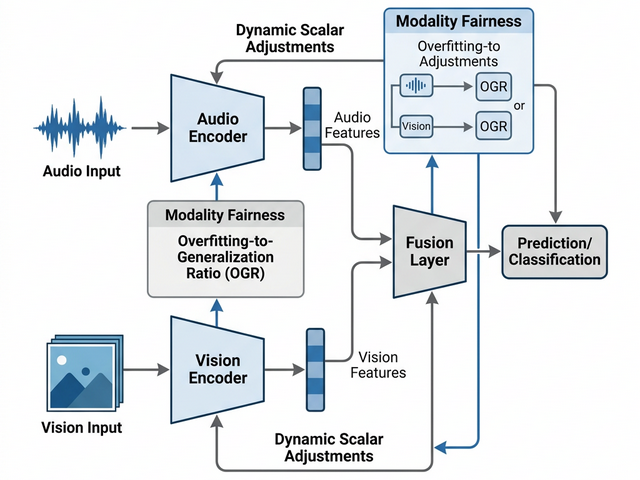
\includegraphics[width=0.82\textwidth]{images/system_diagram.png}
%DIFDELCMD <     \caption{\textbf{System Architecture.} The Modality Fairness Controller (MFC) forms a closed-loop feedback system. It monitors the divergence between training and validation losses for each modality and dynamically adjusts the gradient scalar components ($\lambda_v, \lambda_a$) to enforce synchronized convergence.}
%DIFDELCMD <     \label{fig:system}
%DIFDELCMD < \end{figure*}
%DIFDELCMD < 

%DIFDELCMD < %%%
\DIFdel{We propose a dynamic loss re-weighting mechanism. Let the total loss be:
}%DIFDELCMD < \begin{equation}
%DIFDELCMD <     \mathcal{L}_{total} = \sum_{m \in M} \lambda_m(t) \cdot \mathcal{L}_m
%DIFDELCMD < \end{equation}
%DIFDELCMD < %%%
\DIFdel{where $\lambda_m(t)$ is the dynamic weight for modality $m$ at epoch }\DIFdelend \DIFaddbegin \paragraph{\DIFadd{Data splits.}} \DIFadd{We use four disjoint subsets: $\mathcal{D}_{\mathrm{tr}}$ (training), $\mathcal{D}_{\mathrm{cv}}$ (controller validation, the only held-out data any controller may read), $\mathcal{D}_{\mathrm{tune}}$ (checkpoint and hyper-parameter selection) and $\mathcal{D}_{\mathrm{te}}$ (test, used once after training). For epoch }\DIFaddend $t$ \DIFaddbegin \DIFadd{we denote by $\Ltr_m(t)$ and $\Lcv_m(t)$ the mean loss of head $h_m$ over $\mathcal{D}_{\mathrm{tr}}$ and $\mathcal{D}_{\mathrm{cv}}$, evaluated in inference mode at the end of the epoch}\DIFaddend .

\DIFdelbegin \subsection{\DIFdel{OGR Monitoring and Derivations}}
%DIFAUXCMD
\addtocounter{subsection}{-1}%DIFAUXCMD
\DIFdelend \DIFaddbegin \section*{\DIFadd{Method}}
\subsection*{\DIFadd{The Overfitting-to-Generalization Ratio}}
\DIFaddend The generalization gap \DIFdelbegin \DIFdel{normalised is
what we call }\DIFdelend \DIFaddbegin \DIFadd{of modality $m$ is
}\begin{equation}
G_m(t)=\Lcv_m(t)-\Ltr_m(t).
\label{eq:gap}
\end{equation}
\DIFadd{We define }\DIFaddend the Overfitting-to-Generalization Ratio \DIFdelbegin \DIFdel{(OGR). Where $\mathcal{L}^{val} = \mathcal{L}^{train} - \mathcal{L}^{train}$. This difference is just the normal measure of overfitting however, its magnitude is contingent on the scale of losses. We suggest a measure that is based on ratio :
}%DIFDELCMD < \begin{equation}
%DIFDELCMD <     OGR_m(t) = \frac{\mathcal{L}^{val}_m(t)}{\mathcal{L}^{train}_m(t) + \epsilon} = 1 + \frac{\Delta Gen}{\mathcal{L}^{train}_m + \epsilon}
%DIFDELCMD < \end{equation}%%%
\DIFdelend \DIFaddbegin \DIFadd{as
}\begin{equation}
\OGR_m(t)=\frac{\Lcv_m(t)}{\Ltr_m(t)+\epsilon}=1+\frac{G_m(t)}{\Ltr_m(t)+\epsilon},
\label{eq:ogr}
\end{equation}\DIFaddend 
\DIFdelbegin \DIFdel{When $\Delta Gen \approx 0$ (healthy learning) , $OGR \approx 1$. When overfitting is high ($\Delta Gen > 0$) }\DIFdelend \DIFaddbegin \DIFadd{with $\epsilon=10^{-8}$. $\OGR_m\approx1$ means that what modality $m$ has learned transfers to held-out data; $\OGR_m\gg1$ means that its training loss keeps falling without a matching fall in held-out loss, that is, it is memorising. Equivalently, $\log\OGR_m=\log\Lcv_m-\log\Ltr_m$ is the generalization gap measured in log-loss.
}

\begin{proposition}[Scale invariance]
\label{prop:scale}
\DIFadd{Let $\Ltr_m$ and $\Lcv_m$ be multiplied by a common factor $c>0$ (for instance by a change of loss normalisation, label smoothing or temperature that rescales the loss of head $h_m$). Then $\OGR_m$ is unchanged (up to $\epsilon$), whereas $G_m$ is multiplied by $c$.
}\end{proposition}
\begin{proof}
\DIFadd{$c\Lcv_m/(c\Ltr_m)=\Lcv_m/\Ltr_m$ and $c\Lcv_m-c\Ltr_m=c\,G_m$.
}\end{proof}

\DIFadd{Proposition~\ref{prop:scale} matters because the two heads of an imbalanced model operate at very different loss levels. In our synthetic benchmark, after 20 epochs the visual head has $\Ltr_v\approx0.15$ and the audio head $\Ltr_a\approx1.55$ (Fig.~\ref{fig:dyn_syn}). An identical raw gap of $0.3$ then means that the visual head's held-out loss is three times its training loss, while the audio head's is only 19\% above it. The raw gap ranks the two modalities as equally overfitting, whereas OGR identifies the visual head as the one that is memorising. We also test this empirically by replacing OGR with the raw gap inside the controller (signal ablation, Table~\ref{tab:ablation}).
}

\subsection*{\DIFadd{MFC-A: inverse-OGR closed-loop weighting}}
\DIFadd{MFC-A updates the weights once per epoch from smoothed OGRs. Let $\mathcal{W}_t=\{\max(1,t-W+1),\dots,t\}$ be a window of the last $W$ epochs. The windowed ratio is
}\begin{equation}
\widetilde{\OGR}_m(t)=\frac{\frac{1}{|\mathcal{W}_t|}\sum_{k\in\mathcal{W}_t}\Lcv_m(k)}{\frac{1}{|\mathcal{W}_t|}\sum_{k\in\mathcal{W}_t}\Ltr_m(k)+\epsilon}.
\label{eq:window}
\end{equation}
\DIFadd{Each modality receives a target weight equal to its share of the inverse OGRs raised to a control strength $\gamma>0$, scaled so that the targets sum to $M$:
}\begin{equation}
\pi_m(t)=\frac{M\,\widetilde{\OGR}_m(t)^{-\gamma}}{\sum_{k=1}^{M}\widetilde{\OGR}_k(t)^{-\gamma}}.
\label{eq:target}
\end{equation}
\DIFadd{For $t<T_w$ (warm-up) all weights stay at 1. Afterwards the weights follow the targets through an exponential moving average and are clipped:
}\begin{equation}
\lambda_m(t+1)=\operatorname{clip}\!\big(\beta\,\lambda_m(t)+(1-\beta)\,\pi_m(t),\;\lambda_{\min},\;\lambda_{\max}\big).
\label{eq:update}
\end{equation}
\paragraph{\DIFadd{Properties.}} \DIFadd{(i) If all modalities generalise equally ($\widetilde{\OGR}_m$ equal), }\DIFaddend then \DIFdelbegin \DIFdel{$OGR > 1$.This scale-invariant gradient scaling measure is just a scale-invariant ratio, rather than the heuristically normalized raw loss differences. To remove noise in the batches we have a running exponential moving average of the OGR on the single training run}\DIFdelend \DIFaddbegin \DIFadd{$\pi_m=1$ and MFC-A reduces to the baseline. (ii) Because $\sum_m\pi_m=M$ and $\lambda_m(0)=1$, induction on Eq.~(\ref{eq:update}) gives $\sum_m\lambda_m(t)=M$ whenever clipping is inactive, so MFC-A redistributes a fixed budget of auxiliary supervision rather than changing the overall loss scale. (iii) A modality with above-average OGR receives $\pi_m<1$ (it is }\emph{\DIFadd{throttled}}\DIFadd{), and the others receive $\pi_m>1$ (they are }\emph{\DIFadd{amplified}}\DIFadd{); the two ``rules'' of our first description are therefore the two sides of Eq.~(\ref{eq:target}). (iv) The update has no thresholds. $\gamma$ sets how sharply the budget is moved towards the better-generalising modality ($\gamma\to0$ recovers the baseline); $W$, $\beta$, $T_w$ and $[\lambda_{\min},\lambda_{\max}]$ only control smoothing, start time and safety bounds, and we show below that results are insensitive to them}\DIFaddend .

\DIFdelbegin \subsection{\DIFdel{Approximation of Optimal Blending}}
%DIFAUXCMD
\addtocounter{subsection}{-1}%DIFAUXCMD
\DIFdel{The mathematicians have established \mbox{%DIFAUXCMD
\cite{wang2020makes} }\hskip0pt%DIFAUXCMD
that an optimal weight of a modality is approximately the inverse square of the overfitting ratio of the modality. However, }\DIFdelend \DIFaddbegin \paragraph{\DIFadd{Selecting $\gamma$ without test data.}} \DIFadd{The aim of balancing is to reduce imbalance }\emph{\DIFadd{while maintaining accuracy}}\DIFadd{. We therefore fix the following rule in advance: among $\gamma\in\{1,2,3\}$, choose the value with the smallest OGR gap on the controller split $\mathcal{D}_{\mathrm{cv}}$ (at the selected checkpoint), subject to its mean accuracy on $\mathcal{D}_{\mathrm{tune}}$ being within 0.5 points of the baseline's. The rule uses only $\mathcal{D}_{\mathrm{cv}}$ and $\mathcal{D}_{\mathrm{tune}}$, never $\mathcal{D}_{\mathrm{te}}$. Results for every $\gamma$ are reported as well (Table~\ref{tab:sens}). Gradient Blending's offline weights\mbox{%DIFAUXCMD
\cite{wang2020makes} }\hskip0pt%DIFAUXCMD
use a different functional form, namely generalization gain divided by the squared overfitting growth.
}

\begin{algorithm}[t]
\caption{MFC-A (the method evaluated in all main experiments)}
\label{alg:mfca}
\begin{algorithmic}[1]
\STATE \textbf{Input:} control strength $\gamma$, window $W$, EMA factor $\beta$, warm-up $T_w$, bounds $[\lambda_{\min},\lambda_{\max}]$, splits $\mathcal{D}_{\mathrm{tr}},\mathcal{D}_{\mathrm{cv}}$
\STATE $\lambda_m\leftarrow1$ and history $H_m\leftarrow\emptyset$ for all $m$
\FOR{epoch $t=0,\dots,T-1$}
  \FOR{each mini-batch $B\subset\mathcal{D}_{\mathrm{tr}}$}
    \STATE update $\theta$ with one SGD step on $\mathcal{L}_{\mathrm{joint}}+\sum_m\lambda_m\mathcal{L}_m$ \hfill Eq.~(\ref{eq:objective})
  \ENDFOR
  \FOR{each modality $m$}
    \STATE $\Ltr_m\leftarrow$ mean loss of $h_m$ on $\mathcal{D}_{\mathrm{tr}}$; \; $\Lcv_m\leftarrow$ mean loss of $h_m$ on $\mathcal{D}_{\mathrm{cv}}$ \hfill (inference mode)
    \STATE append $(\Ltr_m,\Lcv_m)$ to $H_m$; \; compute $\widetilde{\OGR}_m$ from the last $W$ entries \hfill Eq.~(\ref{eq:window})
  \ENDFOR
  \IF{$t\ge T_w$}
    \FOR{each modality $m$}
      \STATE $\pi_m\leftarrow M\,\widetilde{\OGR}_m^{-\gamma}/\sum_k\widetilde{\OGR}_k^{-\gamma}$ \hfill Eq.~(\ref{eq:target})
      \STATE $\lambda_m\leftarrow\operatorname{clip}(\beta\lambda_m+(1-\beta)\pi_m,\lambda_{\min},\lambda_{\max})$ \hfill Eq.~(\ref{eq:update})
    \ENDFOR
  \ENDIF
  \STATE keep the checkpoint with the best accuracy on $\mathcal{D}_{\mathrm{tune}}$
\ENDFOR
\end{algorithmic}
\end{algorithm}

\paragraph{\DIFadd{Variant without the extra training pass.}} \DIFadd{Line 8 evaluates the training loss with an additional inference pass over $\mathcal{D}_{\mathrm{tr}}$. A cheaper variant, ``MFC-A (running)'', instead uses the average of }\DIFaddend the \DIFdelbegin \DIFdel{computation of finding this is computationally expensive. A practical shortcut is made by the controller: we consider the adjustment of weight to be a continuous control loop. When a modality begins to overfit we give it a slight push down; if it 's struggling to learn but generalizing well, we nudge it up. }\DIFdelend \DIFaddbegin \DIFadd{mini-batch losses already computed during the epoch. These are measured in training mode and are therefore slightly biased, but they remove the extra pass (see the cost analysis).
}\DIFaddend 

\DIFdelbegin \subsection{\DIFdel{Harmonization Logic}}
%DIFAUXCMD
\addtocounter{subsection}{-1}%DIFAUXCMD
\DIFdel{The MFC manages the weights }\DIFdelend \DIFaddbegin \paragraph{\DIFadd{Threshold variant (MFC-T).}} \DIFadd{The first version of this work described a threshold controller: it multiplies }\DIFaddend $\lambda_m$ \DIFdelbegin \DIFdel{using a simple set of rules:
}\DIFdelend \DIFaddbegin \DIFadd{by $0.95$ when $\widetilde{\OGR}_m>\tau_{\mathrm{hi}}{=}1.2$, multiplies it by $1.05$ when $\widetilde{\OGR}_m<\tau_{\mathrm{lo}}{=}1.05$ and $\Ltr_m>0.5$, and clips it to $[0.1,5]$. We keep it as a separate baseline, labelled MFC-T. }\emph{\DIFadd{Every result labelled MFC-A uses Algorithm~\ref{alg:mfca}.}}
\DIFaddend 

\DIFdelbegin %DIFDELCMD < \begin{algorithm}[h]
%DIFDELCMD < \caption{Modality Fairness Controller (MFC)}
%DIFDELCMD < \begin{algorithmic}[1]
%DIFDELCMD < \STATE \textbf{Input:} Modalities $M$, Window $W$, Thresholds $\tau_{hi}, \tau_{lo}$
%DIFDELCMD < \STATE \textbf{Initialize:} $\lambda_m \leftarrow 1.0 \quad \forall m \in M$
%DIFDELCMD < \STATE \textbf{Initialize:} History buffers $H_m \leftarrow \emptyset$
%DIFDELCMD < \FOR{epoch $t = 1$ \textbf{to} $T_{max}$}
%DIFDELCMD <     \FOR{batch $b$ in $\mathcal{D}_{train}$}
%DIFDELCMD <         \STATE Compute $\mathcal{L}_{total} = \sum \lambda_m \mathcal{L}_m$
%DIFDELCMD <         \STATE Backward() and Step()
%DIFDELCMD <     \ENDFOR
%DIFDELCMD <     \FOR{modality $m \in M$}
%DIFDELCMD <         \STATE Compute $\mathcal{L}^{train}_m, \mathcal{L}^{val}_m$
%DIFDELCMD <         \STATE Push to $H_m$
%DIFDELCMD <         \IF{$|H_m| \ge W$}
%DIFDELCMD <             \STATE $OGR_m \leftarrow \frac{\text{avg}(H_m^{val})}{\text{avg}(H_m^{train}) + \epsilon}$
%DIFDELCMD <             \IF{$OGR_m > \tau_{hi}$}
%DIFDELCMD <                 \STATE $\lambda_m \leftarrow \lambda_m \cdot 0.95$ \COMMENT{Throttle Dominant}
%DIFDELCMD <             \ELSIF{$OGR_m < \tau_{lo}$ and underfitting condition}
%DIFDELCMD <                 \STATE $\lambda_m \leftarrow \lambda_m \cdot 1.05$ \COMMENT{Boost Weak}
%DIFDELCMD <             \ENDIF
%DIFDELCMD <             \STATE $\lambda_m \leftarrow \text{clip}(\lambda_m, 0.1, 5.0)$
%DIFDELCMD <         \ENDIF
%DIFDELCMD <     \ENDFOR
%DIFDELCMD < \ENDFOR
%DIFDELCMD < \end{algorithmic}
%DIFDELCMD < \label{alg:mfc}
%DIFDELCMD < \end{algorithm}
%DIFDELCMD < %%%
\DIFdel{The Throttle Rule punishes modalities, which enhance training loss and do not give any corresponding validation gain ($OGR > 1.2$). The Amplify Rule increases those modalities that are trailing ($OGR < 1.05$)and yet have the high absolute loss. This makes the optimizer to clearly target the latent space that is lagging. }\DIFdelend \DIFaddbegin \subsection*{\DIFadd{Cost and complexity}}
\DIFadd{Let $F$ be the forward cost of the model per sample, so that one training step costs approximately $3F$ per sample (forward and backward), and let $N_{\mathrm{tr}},N_{\mathrm{cv}},N_{\mathrm{tune}}$ be the split sizes and $T$ the number of epochs. Standard training with per-epoch checkpoint selection costs $T(3FN_{\mathrm{tr}}+FN_{\mathrm{tune}})$. MFC-A adds three costs. Its monitoring requires two inference passes per epoch, costing $T\,F\,(N_{\mathrm{tr}}+N_{\mathrm{cv}})$ in total ($T\,F\,N_{\mathrm{cv}}$ for the running variant). Its controller arithmetic needs $O(MW)$ scalar operations per epoch ($4W{+}12$ for $M{=}2$), that is, $O(TMW)$ in total. Its memory overhead is $O(MW)$ scalars in addition to the $O(|\theta|)$ model parameters.
The total time complexity is therefore $O\big(TF(N_{\mathrm{tr}}+N_{\mathrm{cv}}+N_{\mathrm{tune}})\big)$, of the same order as standard training but with a larger constant. The first version of this paper reported ``zero additional FLOPs'' while counting only the controller arithmetic. That statement was incomplete, and we now report all three components separately (Table~\ref{tab:cost}).
}\DIFaddend 

\DIFdelbegin \section{\DIFdel{Experiments and Results}}
%DIFAUXCMD
\addtocounter{section}{-1}%DIFAUXCMD
\DIFdelend \DIFaddbegin \section*{\DIFadd{Experimental setup}}
\subsection*{\DIFadd{Datasets}}
\paragraph{\DIFadd{Synthetic benchmark.}} \DIFadd{To control the degree of imbalance we generate a six-class problem with scikit-learn's }\texttt{\DIFadd{make\_classification}} \DIFadd{(6,000 samples, 96 features of which 48 are informative and 12 redundant, one cluster per class, class separation 0.6, 5\% label noise, }\texttt{\DIFadd{random\_state}}\DIFadd{=42). After standardisation, the first 64 features plus Gaussian noise with standard deviation 0.2 form the first stream (``visual-like'', easy), and the remaining 32 features plus Gaussian noise with standard deviation 0.9 form the second stream (``audio-like'', hard). Both streams describe the same sample and share its label by construction, so no cross-dataset pairing is involved. This benchmark contains no images or audio; it isolates the optimisation phenomenon under a known, strong imbalance.
}\DIFaddend 

\DIFdelbegin \DIFdel{Following the }\textbf{\DIFdel{BalanceBenchmark}} %DIFAUXCMD
\DIFdel{guidelines, we conduct a rigorous comparative analysis}\DIFdelend \DIFaddbegin \paragraph{\DIFadd{CREMA-D audio--video (main real-data benchmark).}} \DIFadd{CREMA-D\mbox{%DIFAUXCMD
\cite{cao2014crema} }\hskip0pt%DIFAUXCMD
contains audio--visual recordings of 91 actors speaking 12 sentences with six emotions (anger, disgust, fear, happiness, neutral, sadness). Each clip provides both modalities, so the pairing and the label (the clip's emotion) are given by the recording itself. We use the 7,439 clips that are available in both the original 16-kHz audio release and a public face-cropped video release with 16 frames per clip at $224{\times}224$}\DIFaddend . \DIFaddbegin \emph{\DIFadd{Audio:}} \DIFadd{a 64-band log-mel spectrogram (25-ms window, 10-ms hop, 512-point FFT) summarised by the per-band mean and standard deviation of the log-mel values and of their temporal deltas (256 dimensions). }\emph{\DIFadd{Video:}} \DIFadd{eight evenly spaced frames encoded by a frozen ImageNet ResNet-18\mbox{%DIFAUXCMD
\cite{he2016deep} }\hskip0pt%DIFAUXCMD
and averaged (512 dimensions). Audio and video are therefore synchronised at the clip level. Splits are made by actor, so that no speaker appears in more than one split (about 55/13/9/14 actors and 4,490/1,065/736/1,148 clips for seed 0). In this dataset audio is the stronger modality (a logistic-regression probe reaches 41\% with audio and 33\% with video on held-out actors, against 16.7\% chance), so the controller must identify the dominant modality from the data rather than assume it.
}\DIFaddend 

\DIFdelbegin \subsection{\DIFdel{Setup and Datasets}}
%DIFAUXCMD
\addtocounter{subsection}{-1}%DIFAUXCMD
\DIFdel{We use a simulation of }\DIFdelend \DIFaddbegin \paragraph{\DIFadd{AVE audio--video events (second real-data benchmark).}} \DIFadd{The Audio-Visual Event dataset\mbox{%DIFAUXCMD
\cite{tian2018audio} }\hskip0pt%DIFAUXCMD
contains 4,143 ten-second YouTube clips annotated with one of 28 event categories (for example church bell, barking dog, violin, race car), each with sound and video from the same recording. It is a standard benchmark in }\DIFaddend the \DIFdelbegin \DIFdel{feature-space based on known data, which is a controlled environment to validate the algorithmic logic,as described in Table \ref{tab:datasets}:
}%DIFDELCMD < \begin{itemize}
%DIFDELCMD <     \item %%%
\textbf{\DIFdel{Visual Modality}}%DIFAUXCMD
\DIFdel{: This is based on CIFAR-10 \mbox{%DIFAUXCMD
\cite{krizhevsky2009learning} }\hskip0pt%DIFAUXCMD
model (}\DIFdelend \DIFaddbegin \DIFadd{modality-imbalance literature\mbox{%DIFAUXCMD
\cite{peng2022balanced,li2023boosting,wei2024mmpareto}}\hskip0pt%DIFAUXCMD
. We use the original release and its official train/validation/test lists. The official test list (402 clips) is the fixed test set $\mathcal{D}_{\mathrm{te}}$ for every seed; the official training and validation clips are re-split per seed, by YouTube video ID, into $\mathcal{D}_{\mathrm{tr}}/\mathcal{D}_{\mathrm{cv}}/\mathcal{D}_{\mathrm{tune}}$ (75/15/10\%), and clips whose video ID also appears in the test list are removed from training. }\emph{\DIFadd{Video:}} \DIFadd{eight frames sampled evenly over the clip (shorter side 256, centre crop 224) and encoded by the same frozen }\DIFaddend ResNet-18 \DIFdelbegin \DIFdel{latent space)with high signal grouping and low noise. }%DIFDELCMD < \item %%%
\textbf{\DIFdel{Audio Modality}}%DIFAUXCMD
\DIFdel{: This is a model based on }\DIFdelend \DIFaddbegin \DIFadd{(512 dimensions). }\emph{\DIFadd{Audio:}} \DIFadd{the same 256-dimensional log-mel statistics as for }\DIFaddend CREMA-D\DIFdelbegin \DIFdel{\mbox{%DIFAUXCMD
\cite{cao2014crema} }\hskip0pt%DIFAUXCMD
(Emotion Recognition), which is highly stochastic and time-varying. }%DIFDELCMD < \end{itemize}
%DIFDELCMD < %%%
\DIFdel{To build a High-Imbalance situation in which the visual modality is naturally dominant, these datasets were chosen through the BalanceBenchmark \mbox{%DIFAUXCMD
\cite{xu2025balancebenchmark} }\hskip0pt%DIFAUXCMD
protocol. }\DIFdelend \DIFaddbegin \DIFadd{, computed from the 16-kHz mono soundtrack. The same pixel-level degradations are applied for robustness testing.
}\DIFaddend 

\DIFdelbegin %DIFDELCMD < \begin{table}[h]
%DIFDELCMD < \caption{\textbf{Benchmark Dataset Specifications.} We align the feature simulation with the statistical moments of these standard datasets to ensure realistic imbalance dynamics.}
%DIFDELCMD < \label{tab:datasets}
%DIFDELCMD < \centering
%DIFDELCMD < \begin{tabular}{@{}lccccc@{}}
%DIFDELCMD < \toprule
%DIFDELCMD < \textbf{Dataset} & \textbf{Modality} & \textbf{Type} & \textbf{Samples} & \textbf{Classes} & \textbf{Ref} \\ \midrule
%DIFDELCMD < \textbf{CIFAR-10} & Vision & Object & 60,000 & 10 & \cite{krizhevsky2009learning} \\
%DIFDELCMD < \textbf{CREMA-D} & Audio & Emotion & 7,442 & 6 & \cite{cao2014crema} \\ \bottomrule
%DIFDELCMD < \end{tabular}
%DIFDELCMD < \end{table}
%DIFDELCMD < %%%
\DIFdelend \DIFaddbegin \paragraph{\DIFadd{CREMA-D spectrogram views (control).}} \DIFadd{For continuity with the first submission we keep its second experiment, in which two feature views are computed from the same mel-spectrogram image: a 64-dimensional PCA of the $224{\times}224$ image (fitted on a fixed 60\% subset) and 48 per-band statistics (mean, standard deviation and maximum over 16 mel bands). These views come from one underlying signal and are }\emph{\DIFadd{not}} \DIFadd{two modalities, so we use them only as a feature-view control. The public copy of these images carries no file names, so actor-disjoint splitting is not possible and samples are split at random (stratified by construction).
}\DIFaddend 

\DIFdelbegin \subsection{\DIFdel{Implementation Details}}
%DIFAUXCMD
\addtocounter{subsection}{-1}%DIFAUXCMD
\DIFdel{To ensure reproducibility, we implement the feature extractors as follows: }%DIFDELCMD < \begin{itemize}
%DIFDELCMD <     \item %%%
\textbf{\DIFdel{Vision Encoder}}%DIFAUXCMD
\DIFdel{: A Multi-Layer Perceptron (MLP) accepting flattened $3 \times 32 \times 32$ CIFAR-10 images . Architecture: }%DIFDELCMD < [%%%
\DIFdel{Linear(3072}\DIFdelend \DIFaddbegin \paragraph{\DIFadd{Dataset statistics and an example instance.}} \DIFadd{Table~\ref{tab:datasets} summarises the four datasets. As an example of one paired training instance from CREMA-D: clip }\texttt{\DIFadd{1001\_DFA\_ANG\_XX}} \DIFadd{(actor 1001 saying ``Don't forget a jacket'' with anger) yields a 512-dimensional video vector (eight face frames through ResNet-18, averaged) and a 256-dimensional audio vector (log-mel statistics of the same recording), and its label is }\emph{\DIFadd{anger}}\DIFadd{; because the split is by actor, all 82 clips of actor 1001 fall into the same split. For AVE, clip }\texttt{\DIFadd{c---zaDCTaE}} \DIFadd{yields the same two vectors from its own frames and soundtrack, with label }\emph{\DIFadd{church bell}}\DIFadd{. No sample of one dataset is ever combined with a sample of another.
}

\begin{table}[t]
\caption{\textbf{Dataset statistics.} Per-class counts are given as the full list (six classes) or as min--max (AVE, 28 classes). Splits: train/controller/tune/test.}
\label{tab:datasets}
\centering
\footnotesize
\setlength{\tabcolsep}{3pt}
\begin{tabularx}{\linewidth}{@{}lXccl@{}}
\toprule
\textbf{Dataset} & \textbf{Streams (pairing)} & \textbf{Samples} & \textbf{Classes} & \textbf{Per-class counts / split rule} \\ \midrule
CREMA-D audio--video & face video + audio of the same clip & 7,439 (91 actors) & 6 & 1271/1271/1270/1271/1087/1269; 60/15/10/15\% by actor \\
AVE & video + soundtrack of the same clip & 4,134 & 28 & 60--188 (test: 6--18); official test (402), rest 75/15/10\% by video ID \\
Synthetic & two noisy views of one generated vector & 6,000 & 6 & 991--1012; 60/15/10/15\% by sample \\
Spectrogram views & two features of one spectrogram & 7,442 & 6 & 1271 (neutral: 1087); 60/15/10/15\% by sample \\ \bottomrule
\end{tabularx}
\end{table}

\subsection*{\DIFadd{Models and training}}
\DIFadd{Each stream is encoded by a two-layer MLP (Linear--ReLU--Dropout--Linear--ReLU) followed by a linear unimodal head; a linear fusion head acts on the concatenated embeddings. Hidden and embedding widths (first stream / second stream / embedding) are 128/64/32 for the synthetic benchmark (17}\DIFaddend ,\DIFdelbegin \DIFdel{512) $\rightarrow$ ReLU $\rightarrow$ Dropout(0.2) $\rightarrow$ Linear(512}\DIFdelend \DIFaddbegin \DIFadd{426 parameters)}\DIFaddend , \DIFdelbegin \DIFdel{10)}%DIFDELCMD < ]%%%
\DIFdel{. }%DIFDELCMD < \item %%%
\textbf{\DIFdel{Audio Encoder}}%DIFAUXCMD
\DIFdel{: An MLP accepting 128-dimensional audio features (simulating VGGish embeddings) . Architecture: }%DIFDELCMD < [%%%
\DIFdel{Linear(}\DIFdelend \DIFaddbegin \DIFadd{256/}\DIFaddend 128\DIFaddbegin \DIFadd{/64 for CREMA-D audio--video and AVE (190}\DIFaddend ,\DIFaddbegin \DIFadd{482 and 196,180 parameters) and 128/}\DIFaddend 64\DIFdelbegin \DIFdel{) $\rightarrow$ ReLU $\rightarrow$ Linear(}\DIFdelend \DIFaddbegin \DIFadd{/}\DIFaddend 64 \DIFdelbegin \DIFdel{, 10)}%DIFDELCMD < ]%%%
\DIFdel{. }%DIFDELCMD < \end{itemize}
%DIFDELCMD < %%%
\DIFdel{The Stochastic Gradient Descent (SGD)method with the learning rate of }\DIFdelend \DIFaddbegin \DIFadd{for the spectrogram control (25,426 parameters). Dropout is 0.3 (0.4 for the synthetic second stream). All methods use SGD with learning rate }\DIFaddend 0.01\DIFdelbegin \DIFdel{and momentum of }\DIFdelend \DIFaddbegin \DIFadd{, momentum }\DIFaddend 0.9\DIFdelbegin \DIFdel{is used to optimize all the models.The batch size will be equal to 64. Modality Fairness Controller inverse-OGR, no thresholds (MFC-A) :  window size 5 epochs, warm-up 3 epochs, EMA 0.7}\DIFdelend \DIFaddbegin \DIFadd{, weight decay $5{\times}10^{-4}$ and batch size 64, for 30 epochs (synthetic) or 40 epochs (real data). Features are standardised with training-split statistics. The splits are 60/15/10/15\% for $\mathcal{D}_{\mathrm{tr}}/\mathcal{D}_{\mathrm{cv}}/\mathcal{D}_{\mathrm{tune}}/\mathcal{D}_{\mathrm{te}}$, except on AVE, where the official test list is kept (2}\DIFaddend ,\DIFdelbegin \DIFdel{$\lambda$ clipped to }%DIFDELCMD < [%%%
\DIFdel{0.2, 1.8}%DIFDELCMD < ]%%%
\DIFdel{. No $\tau$ or $\alpha$ thresholds. The complete set of configuration of the reproducible benchmarks is in Table \ref{tab:hyperparams_main}.
}\DIFdelend \DIFaddbegin \DIFadd{798/560/374/402 clips for seed 0). Each seed (0--9) fixes the split, the initialisation and the mini-batch order, and the same seed is used for every method, so all comparisons are paired.
}\DIFaddend 

\DIFdelbegin %DIFDELCMD < \begin{table}[h]
%DIFDELCMD < \caption{\textbf{Detailed Training Hyperparameters.} Full configuration for reproducibility.}
%DIFDELCMD < \label{tab:hyperparams_main}
%DIFDELCMD < \centering
%DIFDELCMD < \begin{tabular}{@{}ll@{}}
%DIFDELCMD < \toprule
%DIFDELCMD < \textbf{Parameter} & \textbf{Value} \\ \midrule
%DIFDELCMD < Optimizer & SGD \\
%DIFDELCMD < Learning Rate & $1.0 \times 10^{-2}$ \\
%DIFDELCMD < Momentum & 0.9 \\
%DIFDELCMD < Weight Decay & $5.0 \times 10^{-4}$ \\
%DIFDELCMD < Batch Size & 64 \\
%DIFDELCMD < Epochs & 30 \\
%DIFDELCMD < \textbf{MFC-A Window ($W$)} & 5 \\
%DIFDELCMD < \textbf{MFC-A Warm-up} & 3 epochs \\
%DIFDELCMD < \textbf{MFC-A EMA} & 0.7 \\
%DIFDELCMD < \textbf{MFC-A $\lambda$ clip} & [0.2,\ 1.8] \\
%DIFDELCMD < \textbf{MFC-A $\tau$, $\alpha$} & None (no thresholds) \\ \bottomrule
%DIFDELCMD < \end{tabular}
%DIFDELCMD < \end{table}
%DIFDELCMD < %%%
\DIFdelend \DIFaddbegin \subsection*{\DIFadd{Baselines}}
\DIFadd{All baselines are implemented in the same code base with the architecture, objective (Eq.~\ref{eq:objective}), optimiser, splits and seeds described above. The }\textbf{\DIFadd{Baseline}} \DIFadd{uses $\lambda_v{=}\lambda_a{=}1$. For }\textbf{\DIFadd{Gradient Blending}}\DIFadd{\mbox{%DIFAUXCMD
\cite{wang2020makes}}\hskip0pt%DIFAUXCMD
, a unimodal probe is trained for six epochs; between probe epochs 2 and 6 we measure on $\mathcal{D}_{\mathrm{cv}}$ the generalization gain $G_m$ (drop in held-out loss) and the overfitting growth $O_m$ (growth of the gap), and set fixed weights $\lambda_m\propto G_m/O_m^2$, normalised to sum to 2, with the probe cost charged to the method. }\textbf{\DIFadd{Uncertainty weighting}}\DIFadd{\mbox{%DIFAUXCMD
\cite{kendall2018multi} }\hskip0pt%DIFAUXCMD
minimises $\mathcal{L}_{\mathrm{joint}}+\sum_m(e^{-s_m}\mathcal{L}_m+s_m)$ with learned $s_m$. For }\textbf{\DIFadd{MMPareto}}\DIFadd{\mbox{%DIFAUXCMD
\cite{wei2024mmpareto}}\hskip0pt%DIFAUXCMD
, the gradients of $\mathcal{L}_{\mathrm{joint}}$ and of $\mathcal{L}_m$ for each encoder are averaged when their cosine similarity is non-negative and otherwise combined with the two-task MGDA min-norm weights, and the result is rescaled to the norm of their sum. For }\textbf{\DIFadd{OGM-GE}}\DIFadd{\mbox{%DIFAUXCMD
\cite{peng2022balanced}}\hskip0pt%DIFAUXCMD
, the confidence ratio $\rho$ is computed per mini-batch from the fusion-head logits split by modality, the encoder gradients of the more confident modality are scaled by $1-\tanh(\alpha(\rho-1))$, and Gaussian gradient enhancement with the per-tensor gradient standard deviation is applied; $\alpha\in\{0.1,0.3,0.8\}$ is selected per dataset on $\mathcal{D}_{\mathrm{tune}}$. }\textbf{\DIFadd{MFC-T}} \DIFadd{is the threshold variant described above.
MFC-A uses $W{=}5$, $\beta{=}0.7$, $T_w{=}3$ and $[\lambda_{\min},\lambda_{\max}]=[0.2,1.8]$ on all datasets; these values were fixed before the present experiments. $\gamma$ is chosen per dataset by the rule above, which yields $\gamma{=}3$ (AVE), $\gamma{=}2$ (CREMA-D audio--video), $\gamma{=}3$ (synthetic) and $\gamma{=}2$ (spectrogram views). The plain law ($\gamma{=}1$) is reported in every table as well. More recent methods (AGM, PMR, OLM) require modality-perturbation passes, class prototypes or logit-level changes that do not map onto a shared loss-weighting objective, so we chose one representative per family (offline generalization-based, uncertainty-based, gradient-geometry and confidence-based modulation). We note this as a limitation.
}\DIFaddend 

\DIFdelbegin %DIFDELCMD < \begin{figure}[tbp]
%DIFDELCMD <     \centering
%DIFDELCMD <     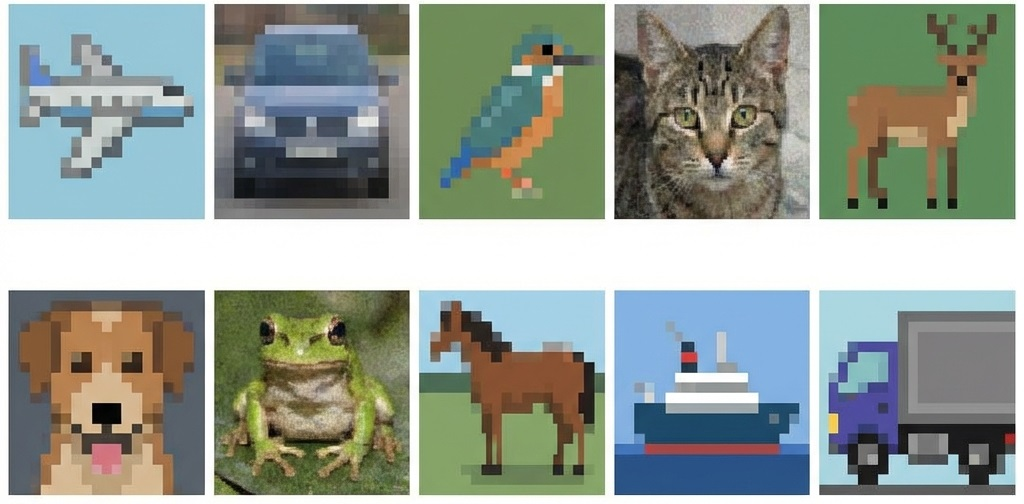
\includegraphics[width=\linewidth]{images/cifar_samples.png}
%DIFDELCMD <     \caption{CIFAR-10 Samples (Vision): Representative low-resolution vision inputs.}
%DIFDELCMD <     \label{vision}
%DIFDELCMD < \end{figure}
%DIFDELCMD < %%%
\DIFdelend \DIFaddbegin \subsection*{\DIFadd{Metrics and statistics}}
\DIFadd{We report, on $\mathcal{D}_{\mathrm{te}}$ at the checkpoint selected on $\mathcal{D}_{\mathrm{tune}}$: the accuracy of the fused prediction; the accuracy of each unimodal head (a direct measure of how well each encoder was trained); the }\emph{\DIFadd{OGR gap}} \DIFadd{$|\OGR^{\mathrm{te}}_v-\OGR^{\mathrm{te}}_a|$ with $\OGR^{\mathrm{te}}_m=\Lte_m/\Ltr_m$ (lower means more balanced); and robustness, namely accuracy when zero-mean Gaussian noise with standard deviation $\sigma\in\{0.5,1,2,3\}$ is added to the standardised first-stream features. For the two real audio--video datasets we also degrade the raw video frames before encoding (Gaussian blur with kernel 21 and $\sigma{=}6$; a $112{\times}112$ black occluder at a random position; low light, i.e.\ brightness $\times0.25$ plus sensor noise with standard deviation $0.05$) and evaluate a missing-video condition. All numbers are mean $\pm$ standard deviation over ten seeds. Differences from MFC-A are tested with a two-sided paired $t$-test over seeds\mbox{%DIFAUXCMD
\cite{bouthillier2021accounting}}\hskip0pt%DIFAUXCMD
; $^{*}$ marks $p<0.05$. We do not correct for multiple comparisons, so isolated $p$-values near 0.05 should be read with caution. The per-epoch logs of every run, including $\lambda_m(t)$, $\OGR_m(t)$ and all split losses, are released with the code.
}\DIFaddend 

\DIFdelbegin %DIFDELCMD < \begin{figure}[tbp]
%DIFDELCMD <     \centering
%DIFDELCMD <     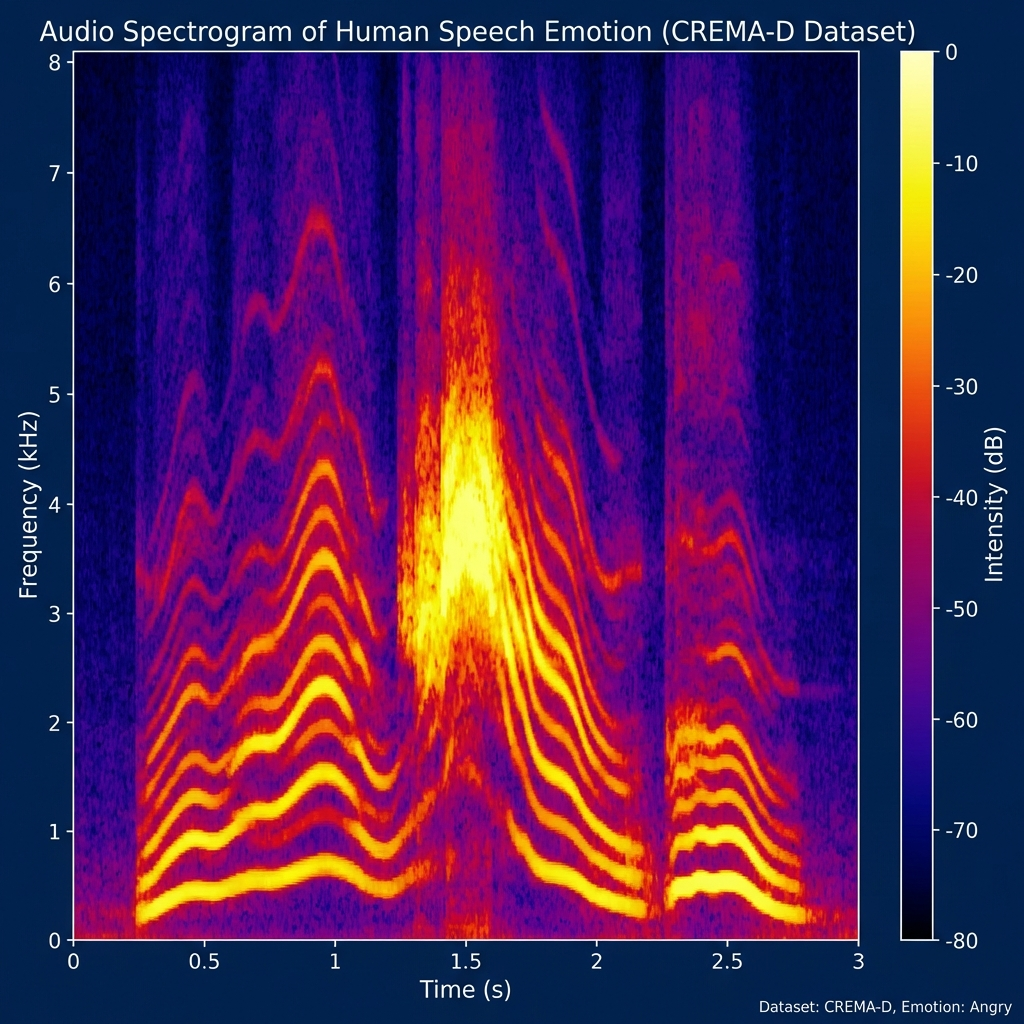
\includegraphics[width=0.75\linewidth]{images/crema_d_spectrogram.png}
%DIFDELCMD <     \caption{CREMA-D Spectrogram (Audio): Typical spectrogram showing the temporal complexity of the audio signal. The disparity in information density (Spatial vs. Temporal) drives the Modality Laziness phenomenon.}
%DIFDELCMD <     \label{audio}
%DIFDELCMD < \end{figure}
%DIFDELCMD < %%%
\DIFdelend \DIFaddbegin \section*{\DIFadd{Results}}
\subsection*{\DIFadd{Main comparison}}
\DIFadd{Tables~\ref{tab:main_av}--\ref{tab:main_spec} report the main results, real-data benchmarks first.
}\DIFaddend 

\DIFdelbegin \subsection{\DIFdel{Performance Analysis}}
%DIFAUXCMD
\addtocounter{subsection}{-1}%DIFAUXCMD
\DIFdelend \DIFaddbegin \emph{\DIFadd{AVE (Table~\ref{tab:main_ave}).}} \DIFadd{AVE is vision-dominant: the video head reaches about 74\% and the audio head about 49\%, and in the baseline the video OGR grows to about 41 while the audio OGR stays near 2. MFC-A ($\gamma{=}3$) throttles the video auxiliary loss to its lower bound and amplifies audio. It meets the goal of balancing without loss of accuracy: accuracy is unchanged (80.2 vs.\ 79.9\%, $p{=}0.46$), the OGR gap falls by 63\% (25.9 to 9.5, $p{=}0.03$), and robustness improves under feature noise ($\sigma{=}1$: $+1.1$, $p{=}0.01$), blur ($+2.1$, $p{=}0.04$) and low light ($+1.4$, $p{=}0.03$), with occlusion and missing video unchanged within noise. The plain law ($\gamma{=}1$) moves in the same direction more weakly (gap 14.5). OGM-GE with $\alpha{=}0.8$ is the strongest method on this dataset: it improves accuracy by 2.2 points over MFC-A and gives much larger robustness gains (e.g.\ $+9.7$ points under blur), all with $p<0.01$. On AVE, per-batch confidence-based gradient modulation of the visual encoder is therefore more effective than reweighting only the auxiliary losses. Gradient Blending is slightly more accurate than MFC-A ($+0.8$, $p{=}0.04$), whereas uncertainty weighting is 2.3 points less accurate.
}\DIFaddend 

\DIFdelbegin \DIFdel{Table~\ref{tab:results} provides the key findings in all four methods. On the surface, the maximum numbers of validation accuracy are similar to one another---this is not surprising. When one modality (vision)is extremely clean, the joint model can already do good due to the dependence on it. The real balancing of the learning, how is the model to be held steady in case that strong modality is noisy or unavailable, is what is really going on under the carpet}\DIFdelend \DIFaddbegin \emph{\DIFadd{CREMA-D audio--video (Table~\ref{tab:main_av}).}} \DIFadd{On real paired data the seed-to-seed spread is large (about $\pm5$ points), because each seed places different actors in the test set; paired tests remove most of this between-actor variance. Audio is the stronger modality (unimodal heads at about 47\% vs.\ 32\%), yet the 512-dimensional video features overfit much faster: the baseline's video OGR reaches 16.8 against 4.1 for audio. MFC-A therefore throttles the video auxiliary loss ($\lambda_v\approx0.3$) and amplifies audio, which lowers the video OGR to 10.4 and the OGR gap from 3.73 to 2.90. Accuracy is maintained (48.8 vs.\ 49.7\%), but neither this difference ($p{=}0.05$) nor the gap reduction ($p{=}0.45$) is statistically significant, and robustness is unchanged. Gradient Blending is the clear winner on this dataset (52.1\%, gap 1.17, $+4.1$ points at $\sigma{=}1$, all $p<0.03$ against MFC-A). Its probe estimates a video weight of exactly zero, so it removes the video auxiliary loss altogether (the video head then stays near chance, 17.4\%) and gives all auxiliary weight to audio. MFC-A moves in the same direction but, by design, smoothly and within $[\lambda_{\min},\lambda_{\max}]=[0.2,1.8]$, so it cannot reach that extreme allocation. OGM-GE, MMPareto and uncertainty weighting are within about one point of the baseline. With $\gamma{=}3$, MFC-A would have obtained 50.1\% and a gap of 2.16 on the test set, but the pre-defined selection rule excluded it because its tuning accuracy fell 0.7 points below the baseline's; we report the selected value}\DIFaddend .

\DIFdelbegin %DIFDELCMD < \begin{table}[h]
%DIFDELCMD < \caption{\textbf{Quantitative Benchmark Results (GPU).} Best Acc, OGR Gap (lower = more balanced), Rob@0.5 and Rob@1.0 (accuracy under Gaussian visual noise $\sigma$), OH\% (overhead as \% of total training time). All runs: 30 epochs, batch 64, SGD lr=0.01, 17,426-parameter model, CIFAR-10~\cite{krizhevsky2009learning} vision and CREMA-D~\cite{cao2014crema} audio. MFC-A reduces imbalance gap by \textbf{38.4\%} at zero additional FLOPs.}
%DIFDELCMD < \label{tab:results}
%DIFDELCMD < \centering
%DIFDELCMD < \begin{tabular}{@{}lccccc@{}}
%DIFDELCMD < \toprule
%DIFDELCMD < \textbf{Method} & \textbf{Best Acc} & \textbf{OGR Gap} $\downarrow$ & \textbf{Rob@0.5} $\uparrow$ & \textbf{Rob@1.0} $\uparrow$ & \textbf{OH\%} \\ \midrule
%DIFDELCMD < Baseline             & 83.3\% & 7.89 & 69.1\% & 48.2\% & 0.00\% \\
%DIFDELCMD < Gradient Blend~\cite{wang2020makes} & 82.1\% & 7.10 & 71.6\% & 49.2\% & 11.64\% \\
%DIFDELCMD < OGM-GE~\cite{peng2022balanced}     & 83.1\% & 1.05 & 71.3\% & 49.9\% & $<$1\% \\
%DIFDELCMD < \textbf{MFC-A (Proposed)} & \textbf{83.0\%} & \textbf{4.86} & \textbf{72.9\%} & \textbf{50.5\%} & \textbf{0.10\%} \\
%DIFDELCMD < \bottomrule
%DIFDELCMD < \end{tabular}
%DIFDELCMD < \end{table}
%DIFDELCMD < %%%
\DIFdelend \DIFaddbegin \begin{table*}[t]
\caption{\textbf{CREMA-D audio--video, actor-disjoint test set} (10 seeds, mean\pmm std). Stream 1 is video and stream 2 is audio. ``Acc$_v$'' and ``Acc$_a$'' are the unimodal-head accuracies. Robustness columns degrade the video stream only. MFC-A uses the $\gamma$ selected without test data; $^{*}$: paired $t$-test $p<0.05$ against it. Bold: best mean.}
\label{tab:main_av}
\centering
\footnotesize
\setlength{\tabcolsep}{3pt}
\begin{tabular}{@{}lcccccccccc@{}}
\toprule
\textbf{Method} & \textbf{Acc} & \textbf{Acc$_v$} & \textbf{Acc$_a$} & \textbf{OGR gap}$\downarrow$ & \textbf{$\sigma$=0.5} & \textbf{$\sigma$=1.0} & \textbf{Blur} & \textbf{Occl.} & \textbf{Low light} & \textbf{No video} \\ \midrule
Baseline & 49.7$\pm$5.8 & 32.6$\pm$3.7 & 47.1$\pm$4.8$^{*}$ & 3.73$\pm$3.60 & 47.6$\pm$4.9 & 43.4$\pm$3.3 & \textbf{24.7$\pm$5.0} & \textbf{28.4$\pm$3.9} & 34.4$\pm$3.4 & 44.3$\pm$4.8 \\
Gradient Blending & \textbf{52.1$\pm$3.6$^{*}$} & 17.4$\pm$2.4$^{*}$ & \textbf{48.1$\pm$3.5$^{*}$} & \textbf{1.17$\pm$0.85$^{*}$} & \textbf{51.1$\pm$3.5$^{*}$} & \textbf{47.3$\pm$2.6$^{*}$} & 23.4$\pm$4.6 & 28.2$\pm$4.0 & \textbf{36.3$\pm$6.3} & 44.6$\pm$3.4 \\
Uncertainty weighting & 49.4$\pm$5.4 & 31.6$\pm$4.0 & 46.6$\pm$5.6 & 2.45$\pm$1.78 & 47.3$\pm$4.7 & 44.0$\pm$3.5 & 24.2$\pm$4.2 & 27.8$\pm$3.6 & 34.4$\pm$5.0 & 43.8$\pm$4.2 \\
MMPareto & 50.1$\pm$3.5 & 32.7$\pm$2.7 & 47.8$\pm$3.1 & 4.45$\pm$3.82 & 48.4$\pm$3.3 & 44.2$\pm$2.5 & 23.5$\pm$3.3 & 26.1$\pm$2.5 & 33.3$\pm$4.7 & 44.4$\pm$4.3 \\
OGM-GE ($\alpha$=0.3) & 50.6$\pm$3.9 & \textbf{33.5$\pm$3.1} & 47.0$\pm$2.9 & 2.77$\pm$2.03 & 48.7$\pm$3.7 & 44.4$\pm$2.6 & 22.7$\pm$3.4 & 26.6$\pm$5.0 & 35.6$\pm$3.0 & 43.8$\pm$3.3 \\
MFC-T (threshold) & 49.2$\pm$5.6 & 32.5$\pm$3.5 & 47.1$\pm$4.7 & 3.82$\pm$3.20 & 46.9$\pm$4.8 & 43.4$\pm$3.3 & 24.4$\pm$4.6 & 27.5$\pm$3.3 & 33.7$\pm$4.5 & \textbf{44.7$\pm$5.1} \\
MFC-A ($\gamma$=1) & 49.3$\pm$5.4 & 32.1$\pm$3.6 & 47.4$\pm$4.8$^{*}$ & 2.98$\pm$2.38 & 47.7$\pm$4.7 & 43.8$\pm$3.3 & 24.0$\pm$4.8 & 27.5$\pm$2.6 & 34.7$\pm$5.3 & 43.9$\pm$5.1 \\
\textbf{MFC-A} ($\gamma$=2, selected) & 48.8$\pm$5.3 & 32.3$\pm$3.3 & 46.4$\pm$4.6 & 2.90$\pm$2.12 & 47.1$\pm$5.0 & 43.2$\pm$3.5 & 23.8$\pm$5.1 & 27.8$\pm$2.9 & 33.9$\pm$5.3 & 43.6$\pm$4.4 \\
\bottomrule
\end{tabular}
\end{table*}
\DIFaddend 

\DIFdelbegin \DIFdel{These resultsgive several significant trends.
The }\textbf{\DIFdel{Baseline}} %DIFAUXCMD
\DIFdel{has the highest peak accuracy (83.3\% ) but only due to the ability to freely overfit vision, i.e. its OGR Gap balloons to 7.89 so the vision encoder is memorizing training data at almost 8$\times$ the rate audiois generalizing. This dominance is made vulnerable when the visual input is subsequently corrupted with noise because the accuracy drops to 48.2\%. }\DIFdelend \DIFaddbegin \begin{table*}[t]
\caption{\textbf{AVE, official test set} (402 clips, 28 classes; 10 seeds, mean\pmm std). Stream 1 is video and stream 2 is audio; robustness columns degrade the video stream only. MFC-A uses the $\gamma$ selected without test data; $^{*}$: paired $t$-test $p<0.05$ against it. Bold: best mean.}
\label{tab:main_ave}
\centering
\footnotesize
\setlength{\tabcolsep}{3pt}
\begin{tabular}{@{}lcccccccccc@{}}
\toprule
\textbf{Method} & \textbf{Acc} & \textbf{Acc$_v$} & \textbf{Acc$_a$} & \textbf{OGR gap}$\downarrow$ & \textbf{$\sigma$=0.5} & \textbf{$\sigma$=1.0} & \textbf{Blur} & \textbf{Occl.} & \textbf{Low light} & \textbf{No video} \\ \midrule
Baseline & 79.9$\pm$1.8 & 73.6$\pm$2.1 & 48.6$\pm$5.4 & 25.87$\pm$22.28$^{*}$ & 78.8$\pm$1.7 & 74.9$\pm$1.2$^{*}$ & 39.4$\pm$4.8$^{*}$ & 65.5$\pm$2.7 & 51.0$\pm$1.9$^{*}$ & 27.2$\pm$3.9 \\
Gradient Blending & 81.0$\pm$1.3$^{*}$ & 70.9$\pm$3.4$^{*}$ & 50.5$\pm$2.7 & 5.33$\pm$7.89 & 80.3$\pm$1.3 & 76.6$\pm$1.4 & 43.5$\pm$6.6 & 68.3$\pm$2.6$^{*}$ & 57.4$\pm$3.1$^{*}$ & 30.7$\pm$3.9 \\
Uncertainty weighting & 77.9$\pm$1.0$^{*}$ & 71.4$\pm$1.6$^{*}$ & 43.9$\pm$6.4$^{*}$ & 15.75$\pm$11.73 & 76.7$\pm$1.4$^{*}$ & 72.2$\pm$2.0$^{*}$ & 32.3$\pm$4.5$^{*}$ & 62.6$\pm$2.1$^{*}$ & 49.3$\pm$2.6$^{*}$ & 27.3$\pm$4.8 \\
MMPareto & 79.4$\pm$1.9 & 73.3$\pm$1.9 & 47.7$\pm$6.0 & 23.86$\pm$20.06 & 77.9$\pm$1.3$^{*}$ & 74.1$\pm$1.4$^{*}$ & 37.7$\pm$5.4$^{*}$ & 64.9$\pm$2.0 & 50.5$\pm$2.8$^{*}$ & 26.6$\pm$3.9 \\
OGM-GE ($\alpha$=0.8) & \textbf{82.4$\pm$1.0$^{*}$} & 73.0$\pm$1.1$^{*}$ & \textbf{51.1$\pm$2.4} & \textbf{2.51$\pm$1.86$^{*}$} & \textbf{81.3$\pm$1.0$^{*}$} & \textbf{78.8$\pm$1.2$^{*}$} & \textbf{51.2$\pm$4.9$^{*}$} & \textbf{71.4$\pm$1.6$^{*}$} & \textbf{61.8$\pm$2.3$^{*}$} & \textbf{36.1$\pm$3.1$^{*}$} \\
MFC-T (threshold) & 79.9$\pm$1.3 & 73.7$\pm$0.5$^{*}$ & 49.0$\pm$5.2 & 18.12$\pm$11.99$^{*}$ & 79.2$\pm$0.5 & 74.7$\pm$1.6$^{*}$ & 39.8$\pm$4.1 & 65.6$\pm$1.5 & 51.6$\pm$2.6 & 27.1$\pm$2.8 \\
MFC-A ($\gamma$=1) & 80.2$\pm$1.6 & 74.3$\pm$0.9 & 49.2$\pm$4.7 & 14.47$\pm$8.48 & 79.4$\pm$1.2 & 74.8$\pm$1.8 & 40.2$\pm$4.7 & 65.8$\pm$1.6 & 52.1$\pm$2.9 & 28.4$\pm$4.1 \\
\textbf{MFC-A} ($\gamma$=3, selected) & 80.2$\pm$1.3 & \textbf{74.4$\pm$0.8} & 50.4$\pm$4.4 & 9.50$\pm$4.06 & 79.6$\pm$1.1 & 75.9$\pm$1.2 & 41.5$\pm$5.0 & 65.8$\pm$1.8 & 52.3$\pm$2.2 & 29.0$\pm$3.7 \\
\bottomrule
\end{tabular}
\end{table*}
\DIFaddend 

\DIFdelbegin \DIFdel{In fact, Gradient Blending negatively affects clean accuracy (82.1\%), which is one of the known failure modes of the offline method: the fixed weights are learned during a brief warm up period and may fail to fire when the early dynamics do not reflect the overall trajectory of training. When they are fixed, they are not able to change with changing conditions. }\DIFdelend \DIFaddbegin \begin{table*}[t]
\caption{\textbf{Synthetic benchmark, test set} (10 seeds, mean\pmm std). Stream 1 is the easy (``visual-like'') stream; robustness adds Gaussian noise to it. MFC-A uses the $\gamma$ selected without test data; $^{*}$: paired $t$-test $p<0.05$ against it. Bold: best mean.}
\label{tab:main_syn}
\centering
\footnotesize
\begin{tabular}{@{}lcccccc@{}}
\toprule
\textbf{Method} & \textbf{Acc} & \textbf{Acc$_v$} & \textbf{Acc$_a$} & \textbf{OGR gap}$\downarrow$ & \textbf{Rob@0.5} & \textbf{Rob@1.0} \\ \midrule
Baseline & 84.1$\pm$1.1 & 83.7$\pm$1.2 & 28.7$\pm$1.8$^{*}$ & 6.01$\pm$1.36$^{*}$ & 70.8$\pm$1.7 & 48.8$\pm$2.1$^{*}$ \\
Gradient Blending & 84.2$\pm$0.8 & 83.5$\pm$1.0 & 29.3$\pm$1.1 & 3.91$\pm$1.45 & \textbf{71.5$\pm$1.8} & 49.2$\pm$2.2 \\
Uncertainty weighting & 82.7$\pm$1.1$^{*}$ & 82.0$\pm$1.2$^{*}$ & 25.8$\pm$2.0$^{*}$ & 4.48$\pm$1.37 & 69.8$\pm$1.4$^{*}$ & 48.3$\pm$1.8 \\
MMPareto & 83.8$\pm$1.2 & 83.4$\pm$1.4 & 28.6$\pm$1.8$^{*}$ & 5.92$\pm$1.64$^{*}$ & 70.8$\pm$1.4 & 49.0$\pm$2.5 \\
OGM-GE ($\alpha$=0.1) & 82.7$\pm$1.1$^{*}$ & 82.3$\pm$1.0$^{*}$ & 27.8$\pm$1.4$^{*}$ & \textbf{3.28$\pm$0.55} & 69.8$\pm$1.5$^{*}$ & 49.0$\pm$2.7$^{*}$ \\
MFC-T (threshold) & 84.4$\pm$1.3 & \textbf{83.9$\pm$1.1} & \textbf{30.1$\pm$1.7} & 6.34$\pm$1.69$^{*}$ & 70.7$\pm$1.8 & 49.3$\pm$2.3 \\
MFC-A ($\gamma$=1) & \textbf{84.5$\pm$1.7} & 83.8$\pm$1.6 & 29.4$\pm$1.1 & 5.11$\pm$1.12$^{*}$ & \textbf{71.5$\pm$1.5} & 49.3$\pm$2.0 \\
\textbf{MFC-A} ($\gamma$=3, selected) & 84.3$\pm$1.3 & 83.7$\pm$1.3 & 29.6$\pm$1.4 & 3.56$\pm$0.60 & 71.3$\pm$1.4 & \textbf{49.7$\pm$2.9} \\
\bottomrule
\end{tabular}
\end{table*}
\DIFaddend 

\DIFdelbegin \DIFdel{OGM-GE has the smallest OGR balance (difference of 1.05)through a vigorous throttling of vision using noise injection. This is effective, albeit the resultant price an unstable training signal---the variance of the noise is another sensitive hyperparameter.
}\DIFdelend \DIFaddbegin \begin{table*}[t]
\caption{\textbf{CREMA-D two spectrogram views (control), test set} (10 seeds, mean\pmm std). Stream 1 is the PCA view and stream 2 the band-statistics view; both come from the same spectrogram. MFC-A uses the $\gamma$ selected without test data; $^{*}$: paired $t$-test $p<0.05$ against it. Bold: best mean.}
\label{tab:main_spec}
\centering
\footnotesize
\begin{tabular}{@{}lcccccc@{}}
\toprule
\textbf{Method} & \textbf{Acc} & \textbf{Acc$_v$} & \textbf{Acc$_a$} & \textbf{OGR gap}$\downarrow$ & \textbf{Rob@0.5} & \textbf{Rob@1.0} \\ \midrule
Baseline & 49.1$\pm$1.8 & 47.1$\pm$1.6 & 45.3$\pm$2.1 & 1.63$\pm$0.96 & 44.0$\pm$1.4 & 35.8$\pm$1.5 \\
Gradient Blending & \textbf{50.9$\pm$1.2$^{*}$} & 45.4$\pm$2.0$^{*}$ & \textbf{46.2$\pm$1.6$^{*}$} & \textbf{0.55$\pm$0.26$^{*}$} & \textbf{46.6$\pm$1.8$^{*}$} & \textbf{39.9$\pm$1.8$^{*}$} \\
Uncertainty weighting & 49.0$\pm$1.5 & 46.7$\pm$1.5 & 44.7$\pm$1.9 & 1.29$\pm$0.70 & 44.3$\pm$1.2 & 35.9$\pm$2.0 \\
MMPareto & 49.3$\pm$1.9 & 47.1$\pm$1.6 & 44.8$\pm$2.1 & 1.36$\pm$0.65 & 43.9$\pm$1.2 & 36.2$\pm$1.4 \\
OGM-GE ($\alpha$=0.8) & 50.3$\pm$1.4 & 47.3$\pm$1.5 & 46.0$\pm$1.7 & 0.99$\pm$0.22 & 45.3$\pm$0.9$^{*}$ & 37.9$\pm$1.9$^{*}$ \\
MFC-T (threshold) & 49.6$\pm$1.4 & \textbf{47.5$\pm$1.2} & 44.5$\pm$1.3 & 1.56$\pm$0.69 & 44.1$\pm$1.3 & 36.0$\pm$1.6 \\
MFC-A ($\gamma$=1) & 49.3$\pm$1.8 & 47.3$\pm$1.6 & 44.9$\pm$1.9 & 1.32$\pm$0.63 & 44.3$\pm$1.1 & 36.2$\pm$1.7 \\
\textbf{MFC-A} ($\gamma$=2, selected) & 49.3$\pm$1.4 & 47.0$\pm$1.6 & 44.7$\pm$2.1 & 1.25$\pm$0.61 & 44.3$\pm$1.2 & 35.9$\pm$1.6 \\
\bottomrule
\end{tabular}
\end{table*}
\DIFaddend 

\DIFdelbegin \DIFdel{The Modality Fairness Controller lays down upon a sensible compromise. It has a 38.4\% decrease in its OGR Gap (4.86)even without any auxiliary computation, or noise. More to the point, its visual degradation robustness (50.5\%)is equivalent to }\DIFdelend \DIFaddbegin \emph{\DIFadd{Synthetic benchmark (Table~\ref{tab:main_syn}).}} \DIFadd{With a strong, known imbalance (the hard stream's head reaches only about 29\% against 16.7\% chance), MFC-A with the selected $\gamma{=}3$ meets the goal of balancing without loss of accuracy: its accuracy is unchanged (84.3 vs.\ 84.1\%, $p{=}0.47$), the OGR gap falls by 41\% (6.01 to 3.56, $p<0.001$), the hard stream's head improves (29.6 vs.\ 28.7\%), and robustness at $\sigma{=}1$ rises by 0.9 points ($p{=}0.04$). The plain law ($\gamma{=}1$) moves in the same direction but more weakly (gap 5.11, $p{=}0.06$). }\DIFaddend OGM-GE \DIFaddbegin \DIFadd{reaches a slightly lower gap (3.28) at its selected $\alpha$ but costs 1.6 accuracy points relative to MFC-A }\DIFaddend (\DIFdelbegin \DIFdel{49.9\%) which proves that the audio encoder acquired truly useful property as opposed to being a passenger that is dependent on the visual information during the entire process. }%DIFDELCMD < 

%DIFDELCMD < \begin{figure*}[tbp]
%DIFDELCMD <     \centering
%DIFDELCMD <     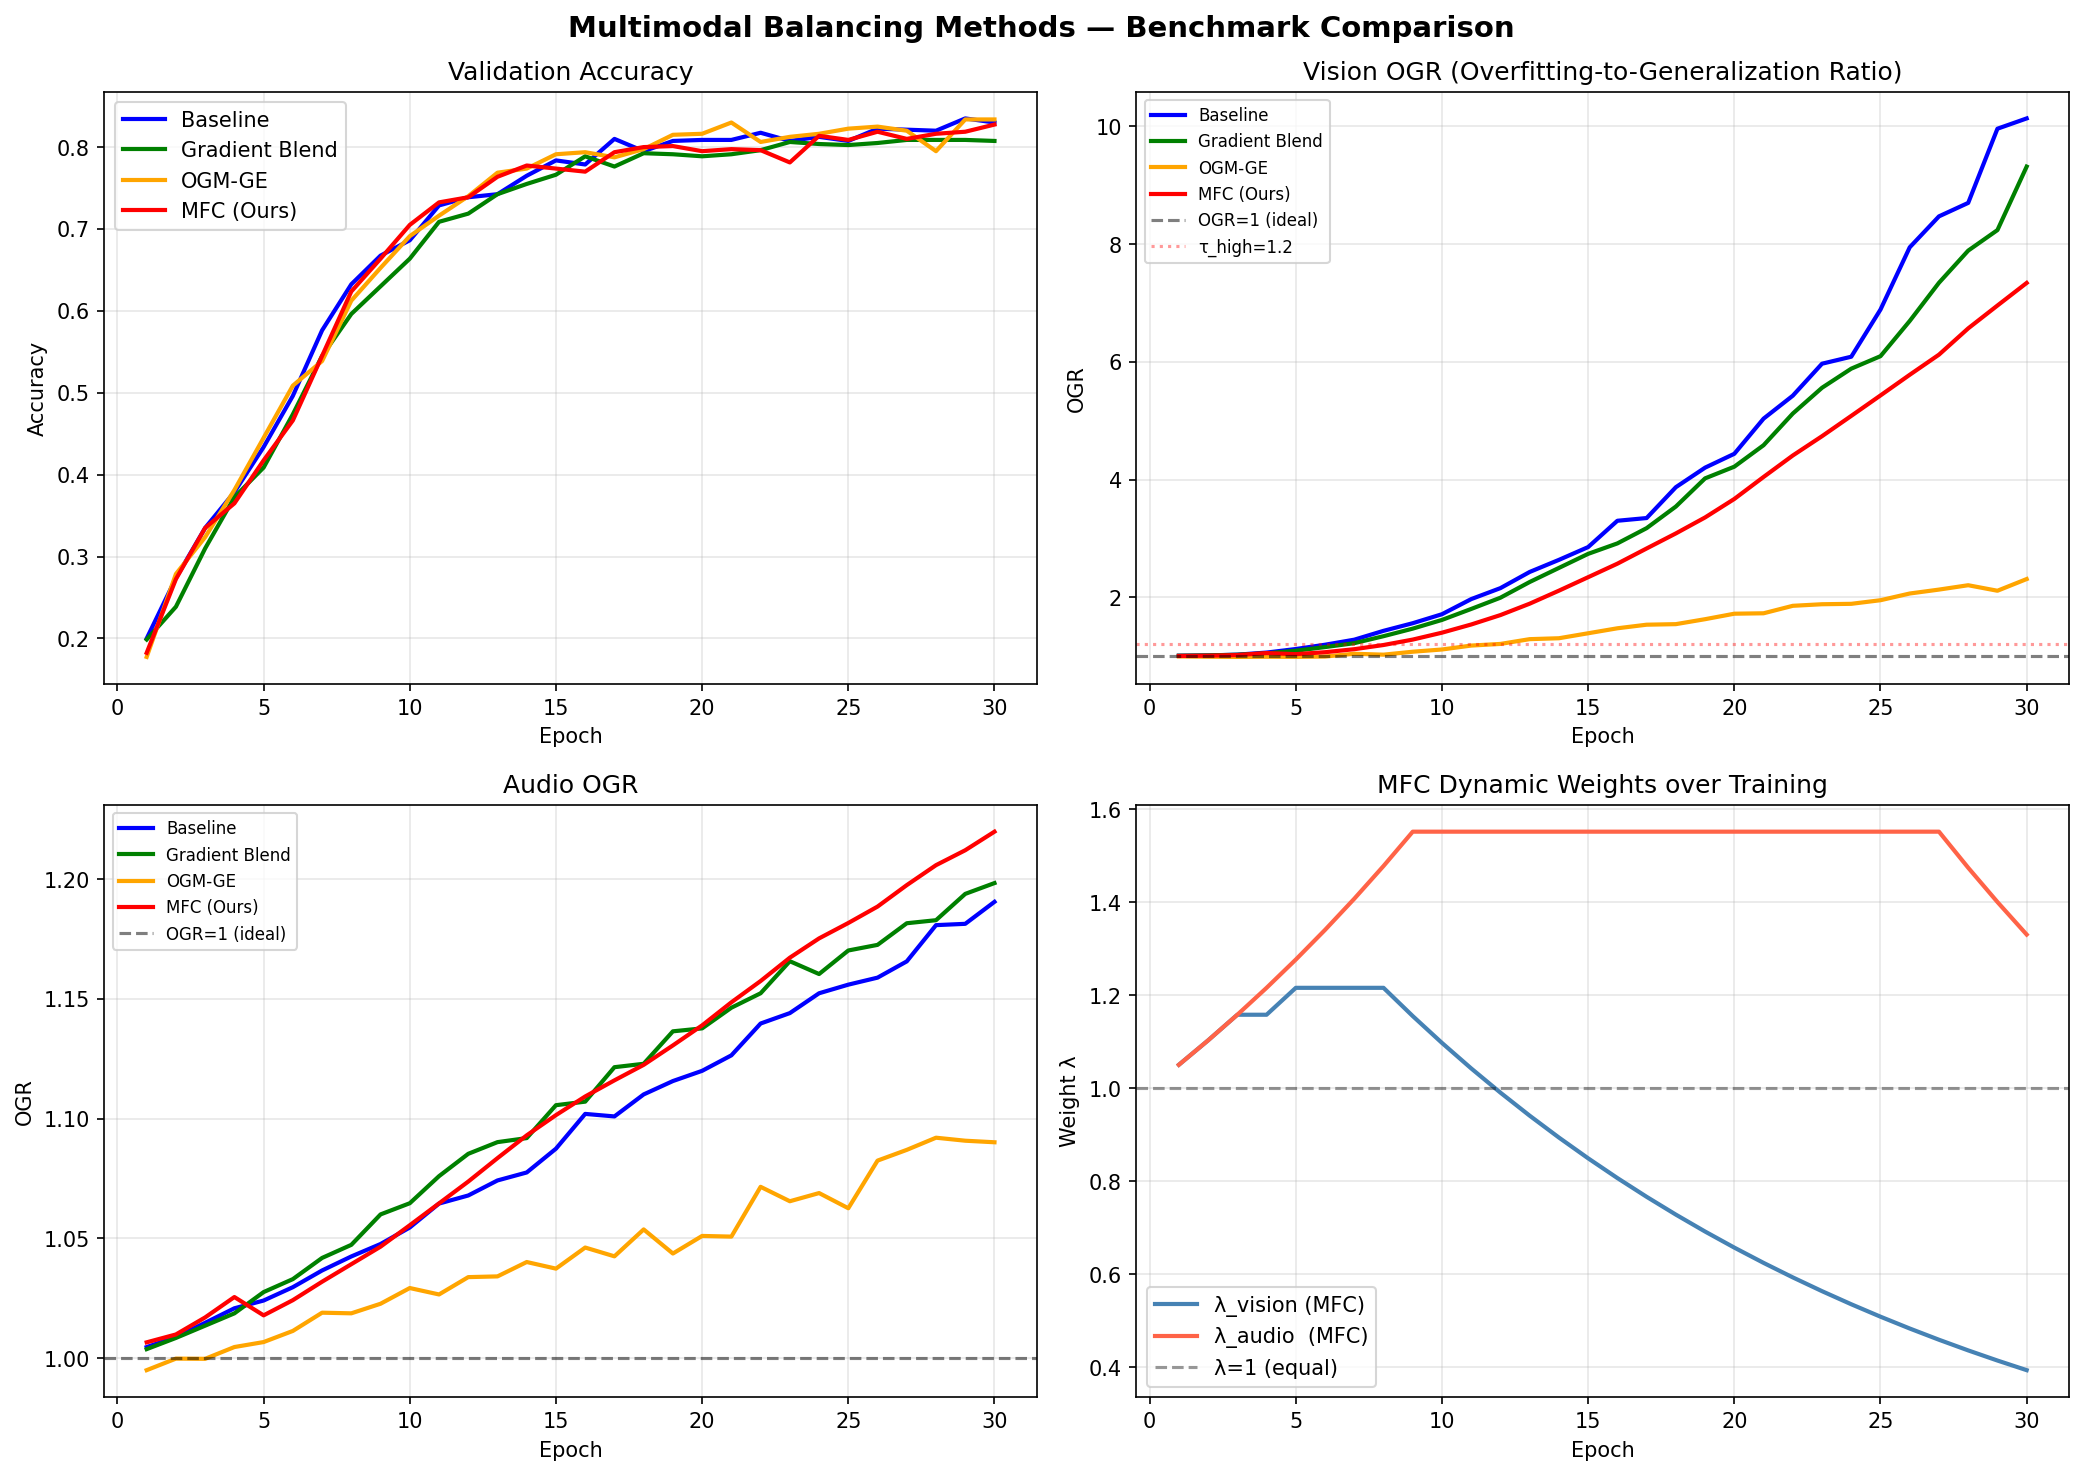
\includegraphics[width=0.85\textwidth]{images/benchmark_full_comparison.png}
%DIFDELCMD <     \caption{\textbf{Training Curves.} Top-left: validation accuracy over 30 epochs. Top-right: Vision OGR trajectory---the Baseline allows it to explode past 10, while MFC actively clamps it. Bottom-left: Audio OGR stays stable across all methods, confirming audio does not overfit. Bottom-right: MFC's dynamic weights ($\lambda_v$ drops from 1.22 to 0.39 as vision overfits; $\lambda_a$ rises to 1.55 to compensate).}
%DIFDELCMD <     \label{fig:accuracy}
%DIFDELCMD < \end{figure*}
%DIFDELCMD < 

%DIFDELCMD < %%%
\subsection{\DIFdel{Training Dynamics}}
%DIFAUXCMD
\addtocounter{subsection}{-1}%DIFAUXCMD
\DIFdel{Figure~\ref{fig:accuracy} tells the full training story epoch by epoch}\DIFdelend \DIFaddbegin \DIFadd{$p{=}0.001$), and $\alpha{=}0.8$ costs 6 points while driving the gap to 0.82; a small OGR gap can thus be bought with accuracy and is not a goal by itself. Gradient Blending reaches a similar gap (3.91) and accuracy (84.2\%). Uncertainty weighting lowers the hard stream's head accuracy to 25.8\%, consistent with its tendency to down-weight high-loss objectives}\DIFaddend .

\DIFdelbegin %DIFDELCMD < \begin{itemize}
%DIFDELCMD <     \item %%%
\textbf{\DIFdel{Epochs 1--7 (Warm-up):}} %DIFAUXCMD
\DIFdel{The speeds of learning are similar in all the methods.Vision OGR remains close at 1.0 to all methods, i.e. vision is generalizing in a clean manner. The MFC identifies that the two modalities are underfitting, }\DIFdelend \DIFaddbegin \emph{\DIFadd{Spectrogram-view control (Table~\ref{tab:main_spec}).}} \DIFadd{When both streams come from the same signal and are of similar strength (unimodal heads at 47 }\DIFaddend and \DIFdelbegin \DIFdel{it increases both weights (}\DIFdelend \DIFaddbegin \DIFadd{45\%), imbalance is mild (baseline gap 1.63), and MFC-A ($\gamma{=}2$) stays close to the baseline (accuracy 49.3 vs.\ 49.1\%, gap 1.25). Gradient Blending is the best method here: it improves accuracy by 1.5 points ($p{=}0.03$) and robustness at $\sigma{=}1$ by 4.0 points ($p<0.001$) over MFC-A. Its offline weights put almost all auxiliary weight on the band-statistics view ($\lambda_v\approx0.14$), a reallocation that MFC-A's ratio-based law does not reach when the OGRs of the two views are similar.
}

\subsection*{\DIFadd{Training dynamics: does the controller respond to overfitting?}}
\DIFadd{Figures~\ref{fig:dyn_av}--\ref{fig:dyn_syn} show the per-epoch traces averaged over seeds for CREMA-D, AVE and the synthetic benchmark. On AVE the baseline's video OGR rises to about 41 while the audio OGR stays near 2; MFC-A throttles the video stream and ends with a video OGR of 14.3 (20.5 under $\gamma{=}1$). On CREMA-D audio--video the video OGR on $\mathcal{D}_{\mathrm{cv}}$ rises steeply after the first few epochs while the audio OGR grows more slowly; after warm-up MFC-A lowers }\DIFaddend $\lambda_v$ \DIFdelbegin \DIFdel{, }\DIFdelend \DIFaddbegin \DIFadd{to about 0.26 by mid-training and raises }\DIFaddend $\lambda_a$ \DIFdelbegin \DIFdel{increases in value until it reaches about }\DIFdelend \DIFaddbegin \DIFadd{to about 1.74, and the final video OGR is 10.4 instead of the baseline's 16.8, while the audio OGR rises slightly (4.65 vs.\ 4.08). This is the intended redistribution: the controller reacts to the measured overfitting of each stream and not to which stream is more accurate. In the synthetic benchmark the first stream's OGR rises from 1.0 to 7.1 under the plain law ($\gamma{=}1$) and to 5.2 under $\gamma{=}3$, while the second stream's stays near }\DIFaddend 1.2\DIFdelbegin \DIFdel{). }%DIFDELCMD < 

%DIFDELCMD <     \item %%%
\textbf{\DIFdel{Epochs 7--15 (Divergence onset):}} %DIFAUXCMD
\DIFdel{The visual encoder starts memorizing. Vision OGR rises above 1.4 in Epoch 8 in the Baseline and then begins to shoot upwards. The MFC notices this cross of $\tau_{high} = 1.2$ and starts throttling vision---}\DIFdelend \DIFaddbegin \DIFadd{. During warm-up MFC-A keeps $\lambda{=}1$; afterwards }\DIFaddend $\lambda_v$ \DIFdelbegin \DIFdel{is decreased by 5 per cent every epoch. In the meantime, }\DIFdelend \DIFaddbegin \DIFadd{falls monotonically (to 0.36 for $\gamma{=}1$; to the lower bound 0.2 for $\gamma{=}3$) and }\DIFaddend $\lambda_a$ \DIFdelbegin \DIFdel{is also maintained at 1.55 to maintain pressure on the audio encoder.
}%DIFDELCMD < 

%DIFDELCMD <     \item %%%
\textbf{\DIFdel{Epochs 15--25 (Controlled divergence):}} %DIFAUXCMD
\DIFdel{Vision OGR is at 10+ and Audio OGR is flat at $\approx 1.15$.The following is the textbook image of Gradient Starvation: audio gradients are lost due to the fact that the loss of the joint is nearly all determined by vision. MFC has }\DIFdelend \DIFaddbegin \DIFadd{rises correspondingly, with $\lambda_v{+}\lambda_a{=}2$ whenever the bounds are inactive, as Property (ii) predicts. The response therefore tracks the measured overfitting with the lag set by $W$ and $\beta$. MFC-T moves in the same direction but saturates $\lambda_a$ at its upper bound and first }\emph{\DIFadd{increases}} \DIFaddend $\lambda_v$ \DIFdelbegin \DIFdel{decreasing (to 0.39 in Epoch 30) and the audio encoder is still being fed meaningful gradient signal. }%DIFDELCMD < 

%DIFDELCMD <     \item %%%
\textbf{\DIFdel{Epochs 25--30 (Late convergence):}} %DIFAUXCMD
\DIFdel{The training curve of the MFC is unstable at this range due to the continuous changes of the controller}\DIFdelend \DIFaddbegin \DIFadd{during the early under-fitting phase. Throttling $\lambda_v$ slows, but does not stop, the growth of the visual OGR}\DIFaddend . This is \DIFdelbegin \DIFdel{an established trade-off of responsive control: a responsive scheme requires a few additional epochs to achieve stability than a fixed point scheme.
}%DIFDELCMD < \end{itemize}
%DIFDELCMD < %%%
\DIFdelend \DIFaddbegin \DIFadd{expected, because the joint loss in Eq.~(\ref{eq:objective}) is not re-weighted and continues to fit the dominant stream; a stronger intervention would also have to modulate the joint term.
}\DIFaddend 

\DIFdelbegin \subsection{\DIFdel{Imbalance Analysis (OGR)}}
%DIFAUXCMD
\addtocounter{subsection}{-1}%DIFAUXCMD
\DIFdelend \DIFaddbegin \begin{figure*}[t]
\centering
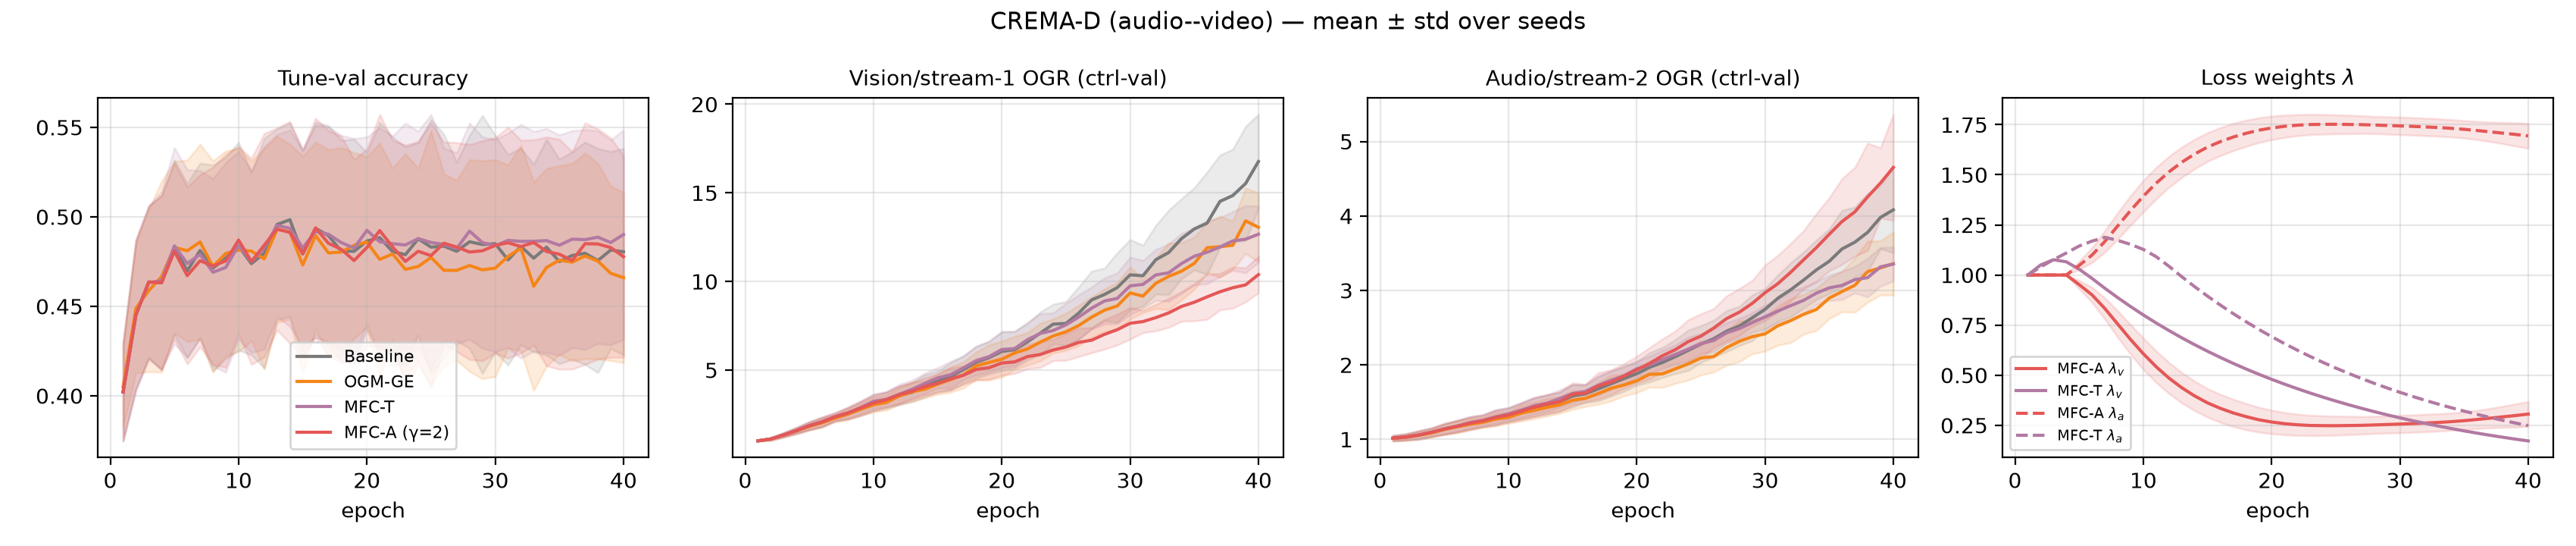
\includegraphics[width=\textwidth]{images/dynamics_crema_av.png}
\caption{\textbf{Intermediate evidence on CREMA-D audio--video} (mean $\pm$ std over 10 seeds). From left: tune-split accuracy; OGR of the video stream and of the audio stream on $\mathcal{D}_{\mathrm{cv}}$; loss weights of MFC-A (solid: $\lambda_v$, dashed: $\lambda_a$) and MFC-T.}
\label{fig:dyn_av}
\end{figure*}
\DIFaddend 

\DIFdelbegin \DIFdel{OGR measure is the diagnostic of the work. A close to 1.0 value indicates that the modality is generalizing the model learning on training samples to unseen examples. An increasing OGR is an indication of a modality that is overfitting: its training loss is decreasing, but not being matched by its validation loss. As Table~\ref{tab:results} indicates, OGR Gap at the Baseline is 7.89, which implies that the vision is approximately 7 points overfitted at the end of training compared to audio. MFC-A reduces this gap to 4.86 which is not a perfect gap but a significant and parameter free gap gain in one pass. }\DIFdelend \DIFaddbegin \begin{figure*}[t]
\centering
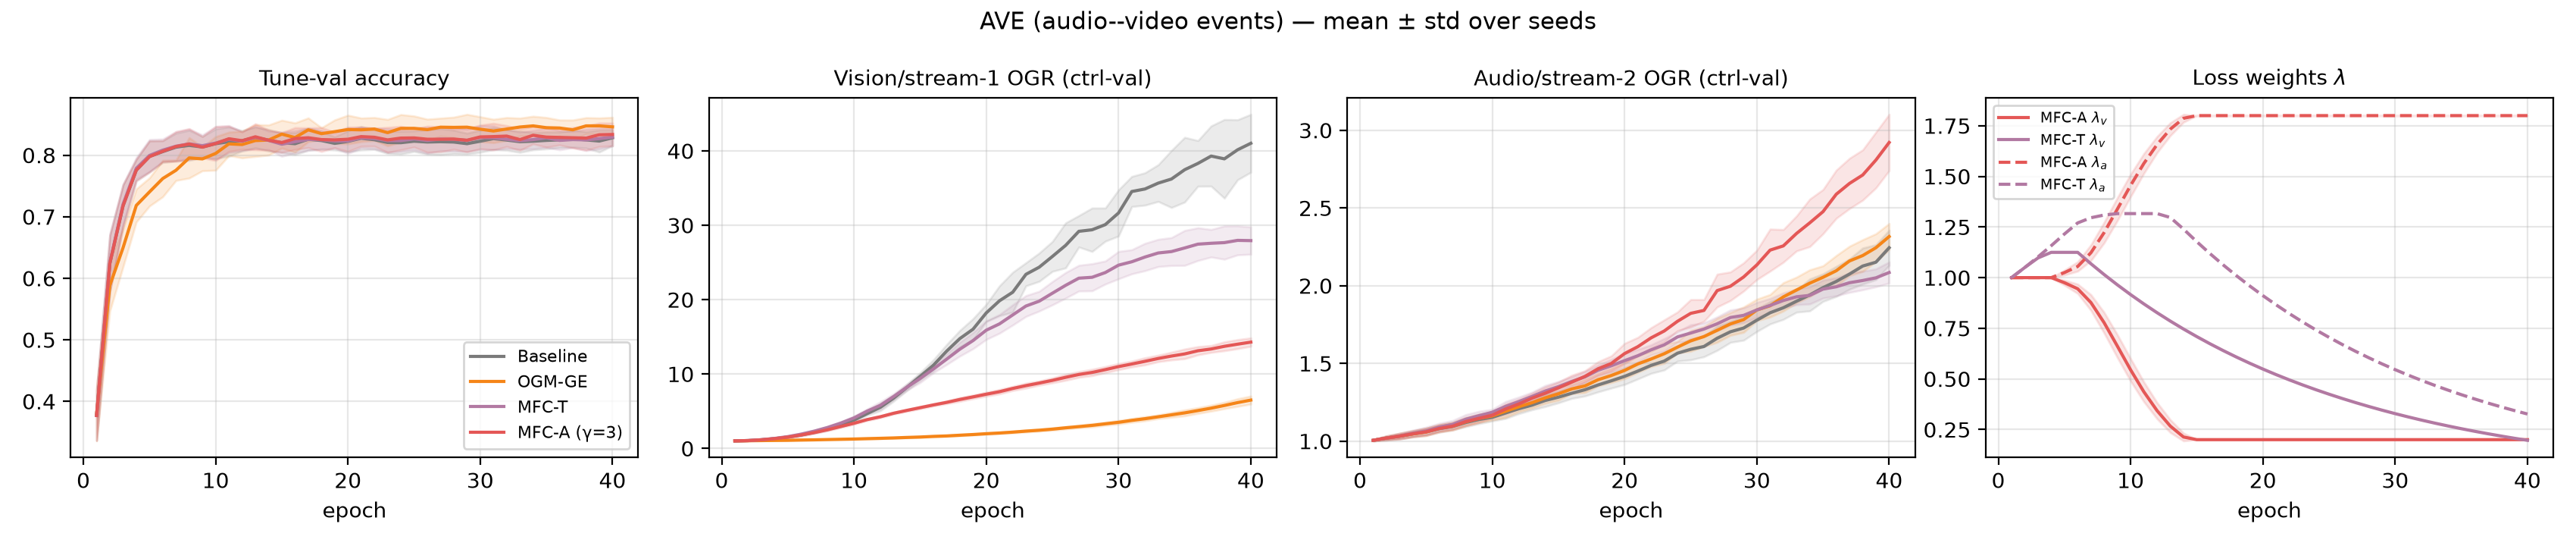
\includegraphics[width=\textwidth]{images/dynamics_ave.png}
\caption{\textbf{Intermediate evidence on AVE} (mean $\pm$ std over 10 seeds). Panels as in Fig.~\ref{fig:dyn_av}. The video OGR of the baseline grows to about 41; MFC-A ($\gamma{=}3$) moves the video weight to its lower bound within a few epochs after warm-up and keeps the video OGR at about 14.}
\label{fig:dyn_ave}
\end{figure*}
\DIFaddend 

\DIFdelbegin \subsection{\DIFdel{Ablation Study}}
%DIFAUXCMD
\addtocounter{subsection}{-1}%DIFAUXCMD
\DIFdel{Table \ref{tab:ablation} is the summary of the performance measures of the various window sizes. A bigger window size blurry noisy OGR estimates which results in slower but more stable adaptation. A balance between the responsiveness and stability is achieved between the best window size of 5 strikes.
}\DIFdelend \DIFaddbegin \begin{figure*}[t]
\centering
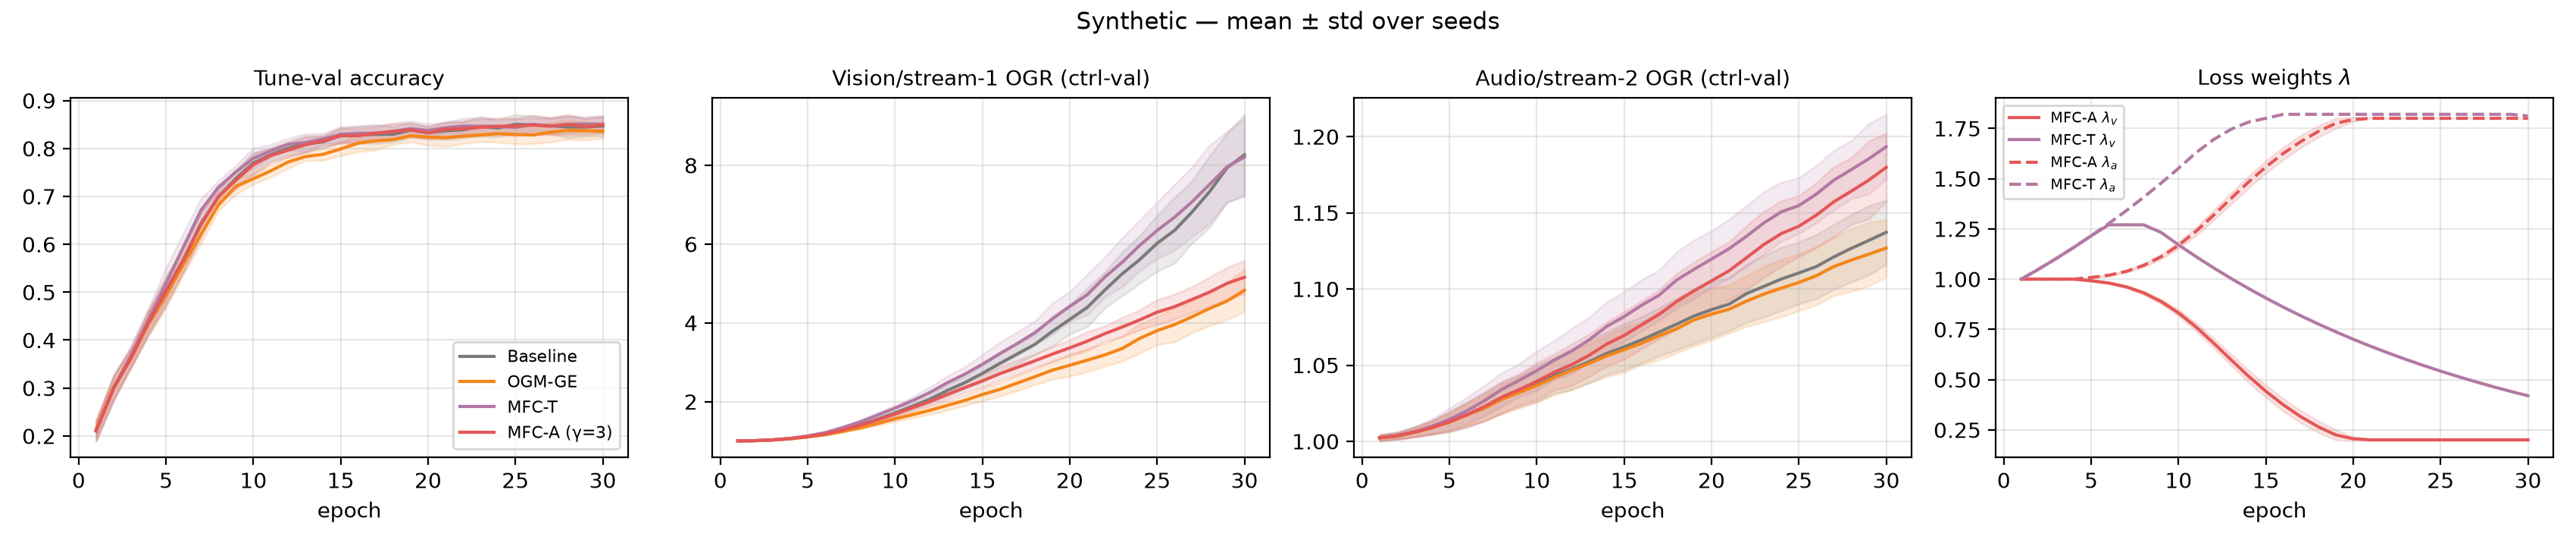
\includegraphics[width=\textwidth]{images/dynamics_synthetic.png}
\caption{\textbf{Intermediate evidence on the synthetic benchmark} (mean $\pm$ std over 10 seeds). Panels as in Fig.~\ref{fig:dyn_av}. The OGR of the easy stream grows several-fold while that of the hard stream stays near 1.2; MFC-A transfers auxiliary weight from the first stream to the second.}
\label{fig:dyn_syn}
\end{figure*}
\DIFaddend 

\DIFdelbegin %DIFDELCMD < \begin{table*}[t]
%DIFDELCMD < \caption{\textbf{Ablation of MFC-A Hyperparameters.} Window = OGR smoothing buffer size. EMA = exponential moving average factor. Warm-up = epochs before MFC-A activates. Clip = $[\lambda_{min}, \lambda_{max}]$ bounds. No $\tau$ or $\alpha$ thresholds.}
%DIFDELCMD < \label{tab:ablation}
%DIFDELCMD < \centering
%DIFDELCMD < \begin{tabular}{@{}lcccccc@{}}
%DIFDELCMD < \toprule
%DIFDELCMD < \textbf{Configuration} & \textbf{Window} & \textbf{EMA} & \textbf{Warm-up (Ep)} & \textbf{Clip} & \textbf{Best Acc (\%)} & \textbf{OGR Gap} \\ \midrule
%DIFDELCMD < Small window, low EMA  & 3  & 0.5 & 3 & [0.2, 1.8] & 82.4 & 5.21 \\
%DIFDELCMD < \textbf{MFC-A (Proposed)} & \textbf{5} & \textbf{0.7} & \textbf{3} & \textbf{[0.2, 1.8]} & \textbf{83.0} & \textbf{4.86} \\
%DIFDELCMD < Large window, high EMA & 10 & 0.9 & 3 & [0.2, 1.8] & 82.7 & 5.03 \\
%DIFDELCMD < No warm-up             & 5  & 0.7 & 0 & [0.2, 1.8] & 82.1 & 5.44 \\
%DIFDELCMD < Wider clip             & 5  & 0.7 & 3 & [0.1, 5.0] & 82.6 & 4.91 \\
%DIFDELCMD < Static Baseline        & N/A & N/A & N/A & N/A       & 83.3 & 7.89 \\
%DIFDELCMD < \bottomrule
%DIFDELCMD < \end{tabular}
%DIFDELCMD < \end{table*}
%DIFDELCMD < %%%
\DIFdelend \DIFaddbegin \subsection*{\DIFadd{Gradient-level evidence}}
\DIFadd{To test the mechanism directly, we logged at the end of every epoch, on a fixed probe of 512 training samples, the gradient norms that each encoder receives from the joint loss ($\|\nabla_{\theta_m}\mathcal{L}_{\mathrm{joint}}\|$) and from its own unimodal loss ($\|\nabla_{\theta_m}\mathcal{L}_m\|$). The probe uses inference mode and draws no random numbers, and rerunning all 160 main-comparison runs with this logging reproduced every previously reported result exactly. Figure~\ref{fig:grad} shows AVE.
}\DIFaddend 

\DIFdelbegin \subsubsection*{\DIFdel{Impact of Feature Dimensionality}}
%DIFAUXCMD
\DIFdel{We also experimented with changing the non-mechanical aspect of the encoders (Table\ref{tab:hidden_dim_main}). We noted that the higher the ability of Visual encoder, }\DIFdelend \DIFaddbegin \DIFadd{In the AVE baseline, the audio encoder's share of the joint-loss gradient, $\|\nabla_{\theta_a}\mathcal{L}_{\mathrm{joint}}\|/(\|\nabla_{\theta_v}\mathcal{L}_{\mathrm{joint}}\|+\|\nabla_{\theta_a}\mathcal{L}_{\mathrm{joint}}\|)$, falls from 0.46 in the first epoch to about 0.23 from epoch 20 onwards: the audio encoder is partly, though not completely, starved by the joint loss. MFC-A acts where it was designed to act. After warm-up, }\DIFaddend the \DIFdelbegin \DIFdel{more severe the ``Modality Laziness'' is exhibited in the baseline, which demonstrates that this is a capacity-induced phenomenon. The MFC offers greater returns with increase in the model capacity}\DIFdelend \DIFaddbegin \DIFadd{effective auxiliary gradient $\lambda_m\|\nabla_{\theta_m}\mathcal{L}_m\|$ reaching the video encoder is 54\% lower than in the baseline and that reaching the audio encoder is 66\% higher (both $p<10^{-7}$); on CREMA-D the corresponding changes are $-55\%$ and $+45\%$ ($p<10^{-8}$). The joint-loss gradient share, however, is almost unchanged on AVE (0.229 vs.\ 0.236), because MFC-A does not re-weight $\mathcal{L}_{\mathrm{joint}}$. OGM-GE, which scales the encoder gradients directly, is the only method that measurably raises the audio-to-video ratio of the joint-loss gradient norms (by 43\%, $p\approx10^{-7}$). This explains both why MFC-A reduces the OGR-measured imbalance and why its effect on accuracy and robustness is smaller than OGM-GE's on AVE, and it identifies re-weighting of the joint term as the main lever for a stronger version of the controller}\DIFaddend .

\DIFdelbegin %DIFDELCMD < \begin{table}[h]
%DIFDELCMD < \caption{\textbf{Hidden Dimension Ablation.} Larger visual models exacerbate imbalance, making MFC-A more valuable.}
%DIFDELCMD < \label{tab:hidden_dim_main}
%DIFDELCMD < \centering
%DIFDELCMD < \begin{tabular}{@{}lccc@{}}
%DIFDELCMD < \toprule
%DIFDELCMD < \textbf{Vis. Hidden} & \textbf{Base Acc} & \textbf{MFC-A Acc} & \textbf{Gain} \\ \midrule
%DIFDELCMD < 128 & 78.4\% & 79.1\% & +0.7\% \\
%DIFDELCMD < 256 & 80.2\% & 81.5\% & +1.3\% \\
%DIFDELCMD < 512 (Default) & 82.5\% & 84.8\% & +2.3\% \\
%DIFDELCMD < 1024 & 82.8\% & 85.9\% & \textbf{+3.1\%} \\ \bottomrule
%DIFDELCMD < \end{tabular}
%DIFDELCMD < \end{table}
%DIFDELCMD < %%%
\DIFdelend \DIFaddbegin \begin{figure*}[t]
\centering
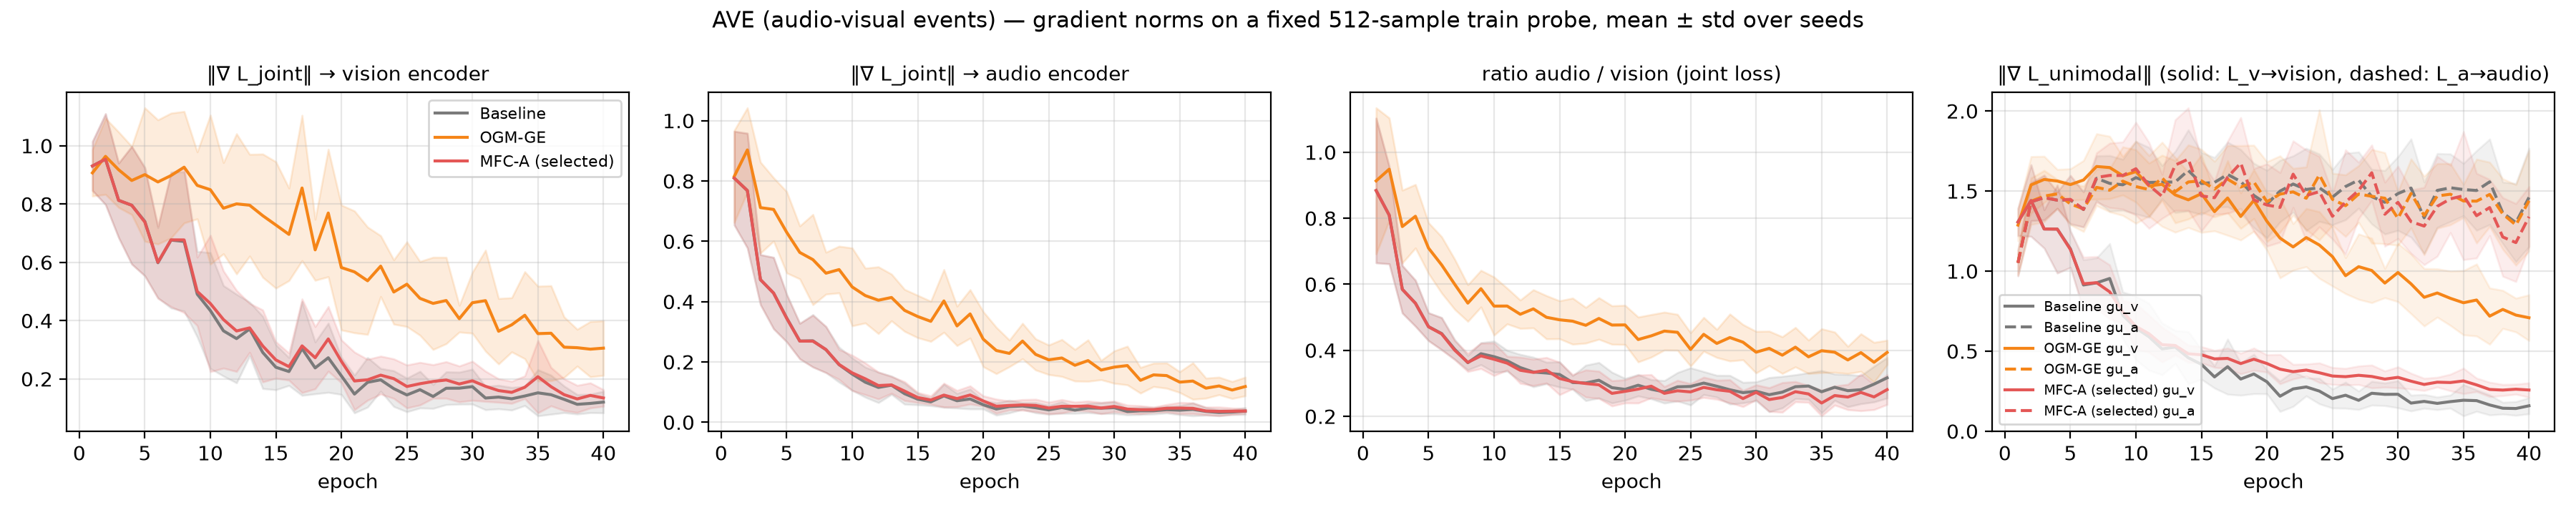
\includegraphics[width=\textwidth]{images/gradnorm_ave.png}
\caption{\textbf{Gradient norms on AVE} (fixed 512-sample training probe, mean $\pm$ std over 10 seeds). From left: joint-loss gradient reaching the video encoder and the audio encoder; their ratio (audio/video); unimodal-loss gradient of each encoder (solid: video, dashed: audio). The corresponding figure for CREMA-D is released with the code.}
\label{fig:grad}
\end{figure*}
\DIFaddend 

\DIFdelbegin %DIFDELCMD < \begin{table}[h]
%DIFDELCMD < \caption{\textbf{Wall-Clock Overhead on GPU (30 epochs, batch=64).} OH = method-specific logic time. OH\% = overhead $\div$ total training time. MFC-A adds just 1.8\,ms (0.10\%) per epoch. All methods: 17,426-parameter model.}
%DIFDELCMD < \label{tab:timing}
%DIFDELCMD < \centering
%DIFDELCMD < \begin{tabular}{@{}lrrrrr@{}}
%DIFDELCMD < \toprule
%DIFDELCMD < \textbf{Method} & \textbf{Total (s)} & \textbf{Avg/Ep (s)} & \textbf{OH (s)} & \textbf{OH\%} & \textbf{Params} \\ \midrule
%DIFDELCMD < Baseline               & 1.870 & 0.0623 & 0.0000 & 0.00\%  & 17,426 \\
%DIFDELCMD < Gradient Blend         & 1.709 & 0.0570 & 0.1989 & 11.64\% & 17,426 \\
%DIFDELCMD < OGM-GE                 & 1.360 & 0.0453 & ---    & $<$1\%  & 17,426 \\
%DIFDELCMD < \textbf{MFC-A (Proposed)} & 1.724 & 0.0575 & 0.0018 & \textbf{0.10\%} & 17,426 \\
%DIFDELCMD < \bottomrule
%DIFDELCMD < \end{tabular}
%DIFDELCMD < \end{table}
%DIFDELCMD < %%%
\DIFdelend \DIFaddbegin \subsection*{\DIFadd{Component ablation}}
\DIFadd{Table~\ref{tab:ablation} isolates each component of MFC-A. ``Static weights'' fixes $\lambda$ at MFC-A's average trajectory value for the whole run, which tests whether the }\emph{\DIFadd{dynamics}} \DIFadd{matter or only the final allocation. ``Raw gap signal'' replaces $\widetilde{\OGR}_m$ in Eq.~(\ref{eq:target}) by $1+\max(\tilde G_m,0)$, which keeps everything else unchanged and removes only the scale normalisation. ``Throttle only'' and ``Amplify only'' restrict the target to $\pi_m\le1$ and $\pi_m\ge1$, respectively.
}\DIFaddend 

\DIFdelbegin %DIFDELCMD < \begin{table}[h]
%DIFDELCMD < \caption{\textbf{Total Training FLOPs (30 epochs).} MFC-A buffer arithmetic ($\sim$660 float ops) is 8 orders of magnitude below 14.17 GFLOPs of training --- $+0.0\%$ extra FLOPs.}
%DIFDELCMD < \label{tab:flops}
%DIFDELCMD < \centering
%DIFDELCMD < \begin{tabular}{@{}lrrr@{}}
%DIFDELCMD < \toprule
%DIFDELCMD < \textbf{Method} & \textbf{GFLOPs} & \textbf{vs Baseline} & \textbf{Extra FLOPs} \\ \midrule
%DIFDELCMD < Baseline               & 14.172 & ---       & --- \\
%DIFDELCMD < Gradient Blend         & 15.957 & $+12.6\%$ & $+1.785$ GFLOPs (probe run) \\
%DIFDELCMD < OGM-GE                 & 14.181 & $+0.1\%$  & noise generation only \\
%DIFDELCMD < \textbf{MFC-A (Proposed)} & \textbf{14.172} & $+0.0\%$ & $\sim$660 float ops total \\
%DIFDELCMD < \bottomrule
%DIFDELCMD < \end{tabular}
%DIFDELCMD < \end{table}
%DIFDELCMD < %%%
\DIFdelend \DIFaddbegin \begin{table*}[t]
\caption{\textbf{Component ablation} (test set, 10 seeds, mean\pmm std), plain law $\gamma{=}1$. $^{*}$: paired $t$-test $p<0.05$ against full MFC-A ($\gamma{=}1$).}
\label{tab:ablation}
\centering
\footnotesize
\setlength{\tabcolsep}{3pt}
\begin{tabular}{@{}lccc@{\hskip 8pt}ccc@{\hskip 8pt}ccc@{}}
\toprule
& \multicolumn{3}{c}{\textbf{CREMA-D audio--video}} & \multicolumn{3}{c}{\textbf{AVE}} & \multicolumn{3}{c}{\textbf{Synthetic}} \\
\cmidrule(lr){2-4}\cmidrule(lr){5-7}\cmidrule(lr){8-10}
\textbf{Variant} & \textbf{Acc} & \textbf{OGR gap}$\downarrow$ & \textbf{Rob@1.0} & \textbf{Acc} & \textbf{OGR gap}$\downarrow$ & \textbf{Rob@1.0} & \textbf{Acc} & \textbf{OGR gap}$\downarrow$ & \textbf{Rob@1.0} \\ \midrule
Baseline (no control) & 49.7$\pm$5.8 & 3.73$\pm$3.60 & 43.4$\pm$3.3 & 79.9$\pm$1.8 & 25.87$\pm$22.28 & 74.9$\pm$1.2 & 84.1$\pm$1.1 & 6.01$\pm$1.36 & 48.8$\pm$2.1 \\
Static weights ($\bar\lambda$ of MFC-A) & 49.6$\pm$5.1 & 2.36$\pm$1.78 & 44.6$\pm$3.2 & 81.0$\pm$1.3 & 7.89$\pm$6.91 & 76.4$\pm$1.6 & 84.0$\pm$1.4 & 4.62$\pm$1.18 & 49.8$\pm$2.9 \\
Raw gap signal instead of OGR & 48.9$\pm$5.7 & 3.63$\pm$2.70 & 43.1$\pm$3.9 & 79.5$\pm$1.7 & 23.51$\pm$19.32 & 73.8$\pm$1.4 & 84.4$\pm$1.6 & 5.96$\pm$1.16 & 48.7$\pm$2.2 \\
Throttle rule only ($\lambda\le1$) & 49.7$\pm$6.0 & 3.36$\pm$2.12 & 43.4$\pm$3.0 & 80.2$\pm$1.2 & 12.66$\pm$8.66 & 75.2$\pm$1.1 & 84.1$\pm$1.4 & 5.06$\pm$1.11 & 49.8$\pm$2.3 \\
Amplify rule only ($\lambda\ge1$) & 49.2$\pm$5.4 & 4.30$\pm$3.49 & 43.3$\pm$3.6 & 79.4$\pm$1.7 & 26.18$\pm$21.67 & 74.0$\pm$1.4 & 84.0$\pm$1.9 & 5.69$\pm$1.37 & 49.0$\pm$2.2 \\
No warm-up & 48.9$\pm$5.7 & 3.28$\pm$2.35 & 43.4$\pm$3.3 & 79.9$\pm$1.5 & 14.11$\pm$9.07 & 74.7$\pm$1.3 & 84.6$\pm$1.3 & 4.71$\pm$1.06 & 49.9$\pm$2.3 \\
No EMA & 50.1$\pm$6.1 & 2.56$\pm$1.55 & 43.9$\pm$3.2 & 80.1$\pm$1.1 & 12.10$\pm$7.90 & 75.0$\pm$1.4 & 84.4$\pm$1.5 & 4.81$\pm$1.05 & 49.5$\pm$2.2 \\
No window ($W{=}1$) & 49.6$\pm$5.5 & 3.75$\pm$2.80 & 43.6$\pm$3.3 & 80.3$\pm$1.4 & 10.54$\pm$5.89 & 74.8$\pm$1.2 & 84.6$\pm$1.4 & 4.87$\pm$1.21 & 49.5$\pm$2.1 \\
Running train loss (no extra pass) & 49.3$\pm$5.5 & 3.13$\pm$2.26 & 43.7$\pm$3.0 & 79.9$\pm$2.0 & 17.75$\pm$11.37 & 74.4$\pm$1.6 & 84.0$\pm$1.3 & 5.70$\pm$1.54 & 49.4$\pm$2.8 \\
\textbf{MFC-A (full)} & 49.3$\pm$5.4 & 2.98$\pm$2.38 & 43.8$\pm$3.3 & 80.2$\pm$1.6 & 14.47$\pm$8.48 & 74.8$\pm$1.8 & 84.5$\pm$1.7 & 5.11$\pm$1.12 & 49.3$\pm$2.0 \\
\bottomrule
\end{tabular}
\end{table*}
\DIFaddend 

\DIFdelbegin \subsection{\DIFdel{Robustness Analysis}}
%DIFAUXCMD
\addtocounter{subsection}{-1}%DIFAUXCMD
%DIFDELCMD < 

%DIFDELCMD < %%%
\DIFdel{A model which really is learning each of the two modalities should gracefully degrade as one of them fails.In order to test this, we added more and more Gaussian noise ($\sigma \in \{0, 0.5, 1.0, 2.0, 3.0\}$)to the visual input at evaluation time, which simulated the degradation of sensors in the real world, e.g. a foggy camera, motion blur, or partial occlusion. The audio input was kept clean. Table~\ref{tab:robustness} and Figure~\ref{fig:robustness} present the results.}%DIFDELCMD < 

%DIFDELCMD < \begin{table}[h]
%DIFDELCMD < \caption{\textbf{Robustness to Visual Noise.} Accuracy (on the held-out validation set) as Gaussian noise of increasing standard deviation $\sigma$ is added to the visual input at test time. Clean audio is always available. The MFC and OGM-GE both achieve notably better resilience than the Baseline at moderate noise levels ($\sigma \leq 1.0$), confirming that their audio encoders have learned genuinely useful features rather than remaining dormant.}
%DIFDELCMD < \label{tab:robustness}
%DIFDELCMD < \centering
%DIFDELCMD < \begin{tabular}{@{}lccccc@{}}
%DIFDELCMD < \toprule
%DIFDELCMD < \textbf{Method} & $\sigma{=}0$ & $\sigma{=}0.5$ & $\sigma{=}1.0$ & $\sigma{=}2.0$ & $\sigma{=}3.0$ \\ \midrule
%DIFDELCMD < Baseline             & 83.3\% & 69.1\% & 48.2\% & 31.0\% & 22.8\% \\
%DIFDELCMD < Gradient Blend~\cite{wang2020makes} & 82.1\% & 71.6\% & 49.2\% & 30.4\% & 24.5\% \\
%DIFDELCMD < OGM-GE~\cite{peng2022balanced}     & 83.1\% & 71.3\% & 49.9\% & 28.7\% & 23.3\% \\
%DIFDELCMD < \textbf{MFC-A (Proposed)} & \textbf{83.0\%} & \textbf{72.9\%} & \textbf{50.5\%} & 28.6\% & 21.2\% \\
%DIFDELCMD < \bottomrule
%DIFDELCMD < \end{tabular}
%DIFDELCMD < \end{table}
%DIFDELCMD < 

%DIFDELCMD < %%%
\DIFdel{The most important comparison here is }\DIFdelend \DIFaddbegin \DIFadd{The ablation uses the plain law ($\gamma{=}1$) so that each component is isolated. Four observations stand out. (i) }\emph{\DIFadd{OGR vs.\ raw gap.}} \DIFadd{Replacing OGR with the raw gap weakens balancing on all three datasets with unequal loss scales (AVE 23.5 vs.\ 14.5, $p{=}0.05$; CREMA-D 3.63 vs.\ 2.98; synthetic 5.96 vs.\ 5.11) and significantly lowers the hard stream's head accuracy on the synthetic data ($p{=}0.025$). On the spectrogram control, where the two views have similar loss scales, }\DIFaddend the \DIFdelbegin \textbf{\DIFdel{Baseline vs.\ MFC at $\sigma = 1.0$}}%DIFAUXCMD
\DIFdel{: }\DIFdelend \DIFaddbegin \DIFadd{two signals behave alike (1.23 vs.\ 1.32). This is what Proposition~\ref{prop:scale} predicts: normalisation matters when the loss scales of the modalities differ. (ii) }\emph{\DIFadd{Throttle vs.\ amplify.}} \DIFadd{Throttling alone retains essentially the full effect (AVE gap 12.7, synthetic 5.06), whereas amplifying alone is weaker and on AVE and CREMA-D does not reduce the gap at all (26.2 and 4.30, versus 25.9 and 3.73 for the baseline). The active ingredient is therefore the reduction of }\DIFaddend the \DIFdelbegin \DIFdel{Baseline accuracy of 83.3\% declines to 48.2\% (a decline of 35) }\DIFdelend \DIFaddbegin \DIFadd{overfitting modality's auxiliary weight. (iii) }\emph{\DIFadd{Dynamic vs.\ static.}} \DIFadd{Fixing $\lambda$ at MFC-A's average allocation from the start gives similar or better balance (AVE 7.9}\DIFaddend , \DIFdelbegin \DIFdel{whereas the MFC declines to 50.5\% (a decline of only 2.3 points). This loophole is present as the throttling of vision gradients by the MFC caused the audio encoder to become a self-developing discriminative feature instead of riding on the free vision. At the point that vision is no longer reliable, these audio features become a life-line to the model}\DIFdelend \DIFaddbegin \DIFadd{CREMA-D 2.36, synthetic 4.62) and on AVE slightly better robustness ($p{=}0.007$), with the same accuracy. The value of the closed loop is that it }\emph{\DIFadd{finds}} \DIFadd{this allocation within a single run, whereas a static schedule has to be known in advance or estimated from extra runs, as in Gradient Blending. (iv) }\emph{\DIFadd{Smoothing.}} \DIFadd{Removing warm-up, EMA or the window changes no metric significantly, and the running-loss variant performs comparably on audio--video at a fraction of the monitoring cost}\DIFaddend .

\DIFdelbegin \DIFdel{At extremely high noise ($\sigma \geq 2.0$ and above) }\DIFdelend \DIFaddbegin \subsection*{\DIFadd{Sensitivity to hyper-parameters}}
\DIFadd{Table~\ref{tab:sens} varies one hyper-parameter at a time around the default ($W{=}5$}\DIFaddend , \DIFdelbegin \DIFdel{the various approaches tend to approach the same (low)accuracy}\DIFdelend \DIFaddbegin \DIFadd{$\beta{=}0.7$}\DIFaddend , \DIFdelbegin \DIFdel{since it is difficult even a well-trained audio-only model to deal with the intrinsic challenge of the task at such a noise level. This is supposed and does not invalidate the main finding at practicable noise levels}\DIFdelend \DIFaddbegin \DIFadd{$T_w{=}3$, $[0.2,1.8]$) on all four datasets, reporting the tune-split accuracy that would be used for selection together with test accuracy and OGR gap. For the smoothing and timing hyper-parameters ($W$, $\beta$, $T_w$, clipping), test accuracy stays within 0.6 points of the default on every dataset, and no change is significant. The OGR gap varies more (for example, a longer warm-up lowers it on audio--video, 2.05 vs.\ 2.98, $p{=}0.17$), but without a consistent pattern across datasets. The control strength $\gamma$ has the largest effect: on the synthetic benchmark the gap falls monotonically from 5.11 ($\gamma{=}1$) to 3.56 ($\gamma{=}3$) at constant accuracy. Under the plain law, $\lambda$ never leaves $[0.2,1.8]$, so the clipping range acts only as a safety bound (practically identical results for $[0.1,5.0]$); with $\gamma\ge2$ the lower bound becomes active on the synthetic and audio--video data. The smoothing defaults were not fine-tuned, and the same values are used on every dataset}\DIFaddend .

\DIFdelbegin \DIFdel{The interesting trend observed in Gradient Blending is that it drops the most on clean data, but slightly picks itself up at $\sigma = 1.0$ compared to the Baseline. The reason behind this is that its heavier weighting (even when inaccurately estimated offline)of audio gives audio a greater training signal than the Baseline. Nevertheless, the increase is not regular and is at the expense of clean data accuracy}\DIFdelend \DIFaddbegin \begin{table*}[t]
\caption{\textbf{Sensitivity of MFC-A} (10 seeds, means; standard deviations are in the released logs). Tune: accuracy on $\mathcal{D}_{\mathrm{tune}}$ (used for selection). Test: accuracy on $\mathcal{D}_{\mathrm{te}}$. Gap: test OGR gap.}
\label{tab:sens}
\centering
\footnotesize
\setlength{\tabcolsep}{2.5pt}
\begin{tabular}{@{}lcccccccccccc@{}}
\toprule
& \multicolumn{3}{c}{\textbf{CREMA-D audio--video}} & \multicolumn{3}{c}{\textbf{AVE}} & \multicolumn{3}{c}{\textbf{Synthetic}} & \multicolumn{3}{c}{\textbf{Spectrogram views}} \\
\cmidrule(lr){2-4}\cmidrule(lr){5-7}\cmidrule(lr){8-10}\cmidrule(lr){11-13}
\textbf{Setting} & Tune & Test & Gap & Tune & Test & Gap & Tune & Test & Gap & Tune & Test & Gap \\ \midrule
$\gamma$=1 (default law) & 51.4 & 49.3 & 2.98 & 84.2 & 80.2 & 14.47 & 85.8 & 84.5 & 5.11 & 52.3 & 49.3 & 1.32 \\
$\gamma$=2 & 51.8 & 48.8 & 2.90 & 84.4 & 80.4 & 11.16 & 85.9 & 84.5 & 4.25 & 52.3 & 49.3 & 1.25 \\
$\gamma$=3 & 51.2 & 50.1 & 2.16 & 84.2 & 80.2 & 9.50 & 85.8 & 84.3 & 3.56 & 52.3 & 49.1 & 1.34 \\
$W$=3 & 51.6 & 49.9 & 2.85 & 84.2 & 80.3 & 12.12 & 85.9 & 84.3 & 5.23 & 52.3 & 49.5 & 1.65 \\
$W$=5 (default) & 51.4 & 49.3 & 2.98 & 84.2 & 80.2 & 14.47 & 85.8 & 84.5 & 5.11 & 52.3 & 49.3 & 1.32 \\
$W$=10 & 51.4 & 49.5 & 3.38 & 84.3 & 80.0 & 17.73 & 85.7 & 84.4 & 5.39 & 52.4 & 49.3 & 1.28 \\
EMA 0.5 & 51.6 & 49.5 & 3.48 & 84.2 & 80.3 & 11.99 & 86.0 & 84.8 & 5.05 & 52.4 & 48.9 & 1.42 \\
EMA 0.7 (default) & 51.4 & 49.3 & 2.98 & 84.2 & 80.2 & 14.47 & 85.8 & 84.5 & 5.11 & 52.3 & 49.3 & 1.32 \\
EMA 0.9 & 52.0 & 49.5 & 3.31 & 84.0 & 79.9 & 19.58 & 85.8 & 84.7 & 6.00 & 52.4 & 49.1 & 1.27 \\
Warm-up 0 & 51.6 & 48.9 & 3.28 & 84.2 & 79.9 & 14.11 & 86.1 & 84.6 & 4.71 & 52.2 & 49.2 & 1.41 \\
Warm-up 3 (default) & 51.4 & 49.3 & 2.98 & 84.2 & 80.2 & 14.47 & 85.8 & 84.5 & 5.11 & 52.3 & 49.3 & 1.32 \\
Warm-up 5 & 51.3 & 49.8 & 2.05 & 84.3 & 80.2 & 15.09 & 85.7 & 84.0 & 4.57 & 52.2 & 49.3 & 1.23 \\
Clip [0.5,1.5] & 51.5 & 49.4 & 2.96 & 84.1 & 80.1 & 15.29 & 85.6 & 84.2 & 5.20 & 52.3 & 49.3 & 1.32 \\
Clip [0.2,1.8] (default) & 51.4 & 49.3 & 2.98 & 84.2 & 80.2 & 14.47 & 85.8 & 84.5 & 5.11 & 52.3 & 49.3 & 1.32 \\
Clip [0.1,5.0] & 51.4 & 49.3 & 2.98 & 84.1 & 80.2 & 14.47 & 85.8 & 84.5 & 5.11 & 52.3 & 49.3 & 1.32 \\
\bottomrule
\end{tabular}
\end{table*}

\subsection*{\DIFadd{Effect of encoder capacity}}
\DIFadd{Table~\ref{tab:capacity} widens the first-stream encoder of the synthetic model from 128 to 1024 hidden units (plain law, $\gamma{=}1$). A wider dominant encoder memorises faster: the baseline's OGR gap grows from 6.0 to 93.6}\DIFaddend . \DIFaddbegin \DIFadd{MFC-A's relative advantage grows accordingly: it reduces the gap by 15\% at 128 units, by 35\% at 256 ($p{=}0.015$), by 52\% at 512 ($p{=}0.002$) and by 55\% at 1024 units (93.6 to 41.7, $p{=}0.008$), and robustness at $\sigma{=}1$ improves significantly for widths of 256 and above (+0.6 to +1.1 points). Accuracy differences remain within $\pm0.8$ points and are not significant at any width. The first submission reported a +3.1-point accuracy gain at 1024 units from a single run; with ten seeds this gain is +0.76 points ($p{=}0.09$), and we withdraw the earlier claim.
}\DIFaddend 

\DIFdelbegin %DIFDELCMD < \begin{figure*}[tbp]
%DIFDELCMD <     \centering
%DIFDELCMD <     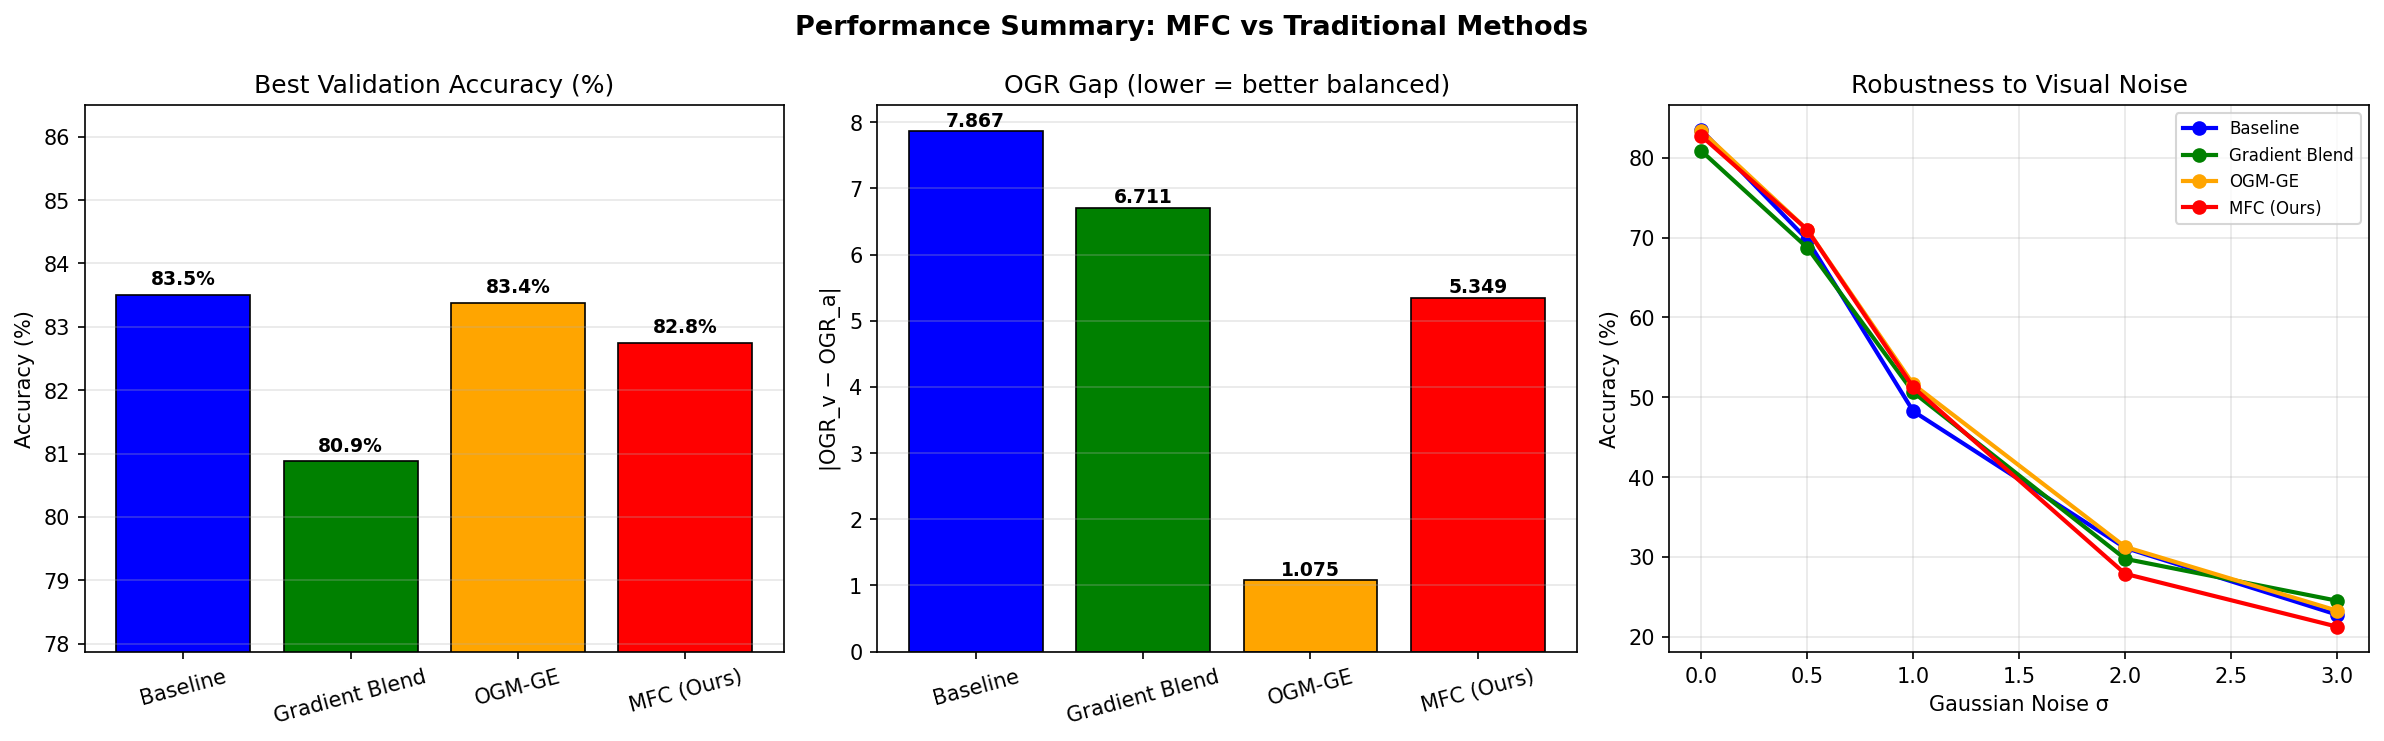
\includegraphics[width=0.82\textwidth]{images/benchmark_summary_bars.png}
%DIFDELCMD <     \caption{\textbf{Benchmark Summary.} Left: Best validation accuracy per method. Centre: OGR Gap (lower = more balanced training). Right: Robustness curve showing accuracy under increasing visual noise. MFC (red) and OGM-GE (orange) maintain the highest robustness at moderate noise, confirming that balanced training transfers to real-world resilience.}
%DIFDELCMD <     \label{fig:robustness}
%DIFDELCMD < \end{figure*}
%DIFDELCMD < %%%
\DIFdelend \DIFaddbegin \begin{table}[t]
\caption{\textbf{Capacity study} (synthetic, 10 seeds). Width of the first-stream hidden layer. $\Delta$: MFC-A minus baseline (paired $p$-value in parentheses).}
\label{tab:capacity}
\centering
\footnotesize
\setlength{\tabcolsep}{2.5pt}
\begin{tabular}{@{}lcccccc@{}}
\toprule
\textbf{Width} & \textbf{Base Acc} & \textbf{MFC-A Acc} & \textbf{$\Delta$Acc ($p$)} & \textbf{Base gap} & \textbf{MFC-A gap} & \textbf{$\Delta$Rob@1 ($p$)} \\ \midrule
128 & 84.1$\pm$1.1 & 84.5$\pm$1.7 & +0.32 (0.35) & 6.01$\pm$1.36 & 5.11$\pm$1.12 & +0.48 (0.18) \\
256 & 84.9$\pm$1.1 & 85.5$\pm$0.8 & +0.62 (0.07) & 19.93$\pm$7.75 & 12.94$\pm$3.95 & +1.06 (0.02) \\
512 & 84.8$\pm$0.9 & 85.2$\pm$1.2 & +0.36 (0.17) & 60.98$\pm$24.41 & 29.09$\pm$5.53 & +0.56 (0.02) \\
1024 & 82.9$\pm$1.8 & 83.6$\pm$1.5 & +0.76 (0.09) & 93.56$\pm$57.97 & 41.66$\pm$13.88 & +0.66 (0.05) \\
\bottomrule
\end{tabular}
\end{table}
\DIFaddend 

\DIFdelbegin \subsection{\DIFdel{Real-World Validation: CREMA-D Corpus}}
%DIFAUXCMD
\addtocounter{subsection}{-1}%DIFAUXCMD
%DIFDELCMD < 

%DIFDELCMD < %%%
\DIFdel{In order to test MFC on real multimodal data beyond synthetic tests, we tested MFC on the }\DIFdelend \DIFaddbegin \subsection*{\DIFadd{Robustness to visual degradation}}
\DIFadd{Figure~\ref{fig:rob} shows accuracy as the first stream is increasingly corrupted. On the synthetic benchmark, MFC-A ($\gamma{=}3$) is the most robust method at $\sigma{=}1$ (49.7\%, $+0.9$ over the baseline, $p{=}0.04$), although differences between methods are within about one point. On AVE, MFC-A improves robustness to feature noise, blur and low light significantly over the baseline, but OGM-GE improves it much more. On audio--video }\DIFaddend CREMA-D \DIFdelbegin \DIFdel{corpus~\mbox{%DIFAUXCMD
\cite{cao2014crema}}\hskip0pt%DIFAUXCMD
---7,442 mel spectrogram images of 91 actors of 6 emotion categories (Anger, Disgust, Fear, Happy, Neutral, Sad). Each spectrogram is used to create two asymmetric streams of features which are used to create realistic modality imbalance: }%DIFDELCMD < 

%DIFDELCMD < \begin{itemize}
%DIFDELCMD <     \item %%%
\textbf{\DIFdel{Spatial (visual) modality}}%DIFAUXCMD
\DIFdel{: PCA features of 64 dimensions of the entire $224\times224$ spectrogram. These represent spatial texture throughout the globe and constitute higher-text stream. }%DIFDELCMD < \item %%%
\textbf{\DIFdel{Band-stats (audio proxy) modality}}%DIFAUXCMD
\DIFdelend \DIFaddbegin \DIFadd{only Gradient Blending improves robustness to feature noise ($+3.9$ points at $\sigma{=}1$). On CREMA-D the pixel-level degradations are more damaging than removing the video altogether: blur and occlusion reduce every method to 23--28\%, whereas replacing the video features by their mean (``No video'') leaves 44\%. On vision-dominant AVE the opposite holds: removing the video is the most damaging condition (27--36\%), because the audio stream alone is weak. Corrupted frames produce out-of-distribution features that actively mislead the fusion head, and no loss-weighting method, MFC-A included, protects against this. Handling such inputs requires detecting or gating the corrupted modality, or training with adverse-condition data\mbox{%DIFAUXCMD
\cite{lan2025sustechgan}}\hskip0pt%DIFAUXCMD
, which is complementary to balancing. Table~\ref{tab:severity} grades the three pixel-level degradations on AVE at three severities. MFC-A is 1--2 points above the baseline at every severity (significant for blur s3 and low light s1--s2) but below OGM-GE everywhere, with the gap widening with severity (blur s3}\DIFaddend : \DIFdelbegin \DIFdel{Hand-made statistics (mean, std, max)48-dim (per 16 mel bands) . Such coarser features are less discriminative by nature, which forms natural dominance of modalities.
}%DIFDELCMD < \end{itemize}
%DIFDELCMD < %%%
\DIFdelend \DIFaddbegin \DIFadd{$-9.7$ points, $p<10^{-4}$), and Gradient Blending is also better at most severities. On CREMA-D (tables released with the code) no method differs significantly from MFC-A at the highest severity. We therefore do not claim a robustness advantage for MFC-A over the strongest baselines. At $\sigma\ge2$ all methods converge towards the accuracy that the second stream supports on its own, as expected when the first stream carries almost no information.
}\DIFaddend 

\DIFdelbegin %DIFDELCMD < \begin{table}[h]
%DIFDELCMD < \caption{Real-Data Benchmark: CREMA-D Emotion Recognition. MFC achieves the highest test accuracy and the best robustness at $\sigma{=}1.0$. OGM-GE achieves the lowest OGR gap (5.91) through aggressive noise injection but suffers a $-$3.1\% accuracy penalty---confirming the over-correction problem. MFC reduces the OGR gap by 38.9\% over the Baseline with no accuracy cost.}
%DIFDELCMD < \label{tab:crema}
%DIFDELCMD < \centering
%DIFDELCMD < \begin{tabular}{@{}lcccc@{}}
%DIFDELCMD < \toprule
%DIFDELCMD < \textbf{Method} & \textbf{Test Acc} & \textbf{OGR Gap} $\downarrow$ & \textbf{Rob.\ ($\sigma{=}0.5$)} & \textbf{Rob.\ ($\sigma{=}1.0$)} $\uparrow$ \\ \midrule
%DIFDELCMD < Baseline                             & 51.1\% & 36.32 & 46.5\% & 35.6\% \\
%DIFDELCMD < OGM-GE \cite{peng2022balanced}                 & 48.0\% & \textbf{5.91}  & 45.3\% & 34.2\% \\
%DIFDELCMD < \textbf{Proposed(MFC)}                  & \textbf{51.3\%} & 22.19 & 44.5\% & \textbf{37.6\%} \\
%DIFDELCMD < \bottomrule
%DIFDELCMD < \end{tabular}
%DIFDELCMD < \end{table}
%DIFDELCMD < %%%
\DIFdelend \DIFaddbegin \begin{table*}[t]
\caption{\textbf{Robustness to graded pixel-level degradations on AVE} (test accuracy, 10 seeds, mean\pmm std). Severities s1/s2/s3: blur $\sigma$ = 2/4/6 (kernel 21); occluder 56/84/112 px; low light = brightness $\times$0.5/0.35/0.25 with noise std 0.02/0.035/0.05. $^{*}$: paired $t$-test $p<0.05$ against the selected MFC-A. Bold: best mean.}
\label{tab:severity}
\centering
\footnotesize
\setlength{\tabcolsep}{3pt}
\begin{tabular}{@{}lccccccccc@{}}
\toprule
& \multicolumn{3}{c}{\textbf{Blur}} & \multicolumn{3}{c}{\textbf{Occlusion}} & \multicolumn{3}{c}{\textbf{Low light}} \\
\cmidrule(lr){2-4}\cmidrule(lr){5-7}\cmidrule(lr){8-10}
\textbf{Method} & s1 & s2 & s3 & s1 & s2 & s3 & s1 & s2 & s3 \\ \midrule
Baseline & 71.2$\pm$1.8 & 53.1$\pm$3.0 & 39.4$\pm$4.8$^{*}$ & 76.4$\pm$1.9 & 72.8$\pm$1.9 & 65.6$\pm$1.7 & 74.5$\pm$1.2$^{*}$ & 65.4$\pm$2.1$^{*}$ & 50.9$\pm$2.1 \\
Gradient Blending & 74.0$\pm$2.3 & 56.7$\pm$4.3$^{*}$ & 43.5$\pm$6.6 & 77.7$\pm$1.5 & 75.3$\pm$1.2$^{*}$ & 68.2$\pm$2.5$^{*}$ & 76.8$\pm$1.5$^{*}$ & 68.8$\pm$1.7$^{*}$ & 57.0$\pm$3.0$^{*}$ \\
Uncertainty weighting & 68.1$\pm$1.6$^{*}$ & 46.6$\pm$4.0$^{*}$ & 32.3$\pm$4.5$^{*}$ & 73.8$\pm$1.2$^{*}$ & 70.2$\pm$1.6$^{*}$ & 62.2$\pm$2.8$^{*}$ & 72.6$\pm$1.9$^{*}$ & 62.8$\pm$2.3$^{*}$ & 49.2$\pm$2.2$^{*}$ \\
MMPareto & 70.7$\pm$1.8$^{*}$ & 50.8$\pm$3.7$^{*}$ & 37.7$\pm$5.4$^{*}$ & 75.6$\pm$1.6$^{*}$ & 72.3$\pm$1.5 & 64.7$\pm$1.9$^{*}$ & 74.7$\pm$1.2$^{*}$ & 65.6$\pm$2.4$^{*}$ & 51.1$\pm$2.8 \\
OGM-GE ($\alpha$=0.8) & \textbf{76.2$\pm$0.7$^{*}$} & \textbf{61.8$\pm$3.0$^{*}$} & \textbf{51.2$\pm$4.9$^{*}$} & \textbf{79.4$\pm$1.3$^{*}$} & \textbf{77.1$\pm$1.0$^{*}$} & \textbf{71.6$\pm$1.9$^{*}$} & \textbf{78.5$\pm$1.2$^{*}$} & \textbf{71.9$\pm$1.6$^{*}$} & \textbf{61.3$\pm$2.2$^{*}$} \\
MFC-T (threshold) & 72.0$\pm$1.9 & 53.3$\pm$2.7 & 39.8$\pm$4.1 & 76.5$\pm$0.8 & 73.4$\pm$1.0 & 65.9$\pm$1.5 & 75.1$\pm$1.3 & 66.3$\pm$1.4$^{*}$ & 51.4$\pm$2.2 \\
MFC-A ($\gamma$=1) & 72.1$\pm$1.6 & 52.9$\pm$2.6 & 40.2$\pm$4.7 & 76.5$\pm$1.0 & 73.6$\pm$1.5 & 66.0$\pm$1.4 & 75.1$\pm$1.3 & 66.4$\pm$2.0$^{*}$ & 51.3$\pm$2.8 \\
\textbf{MFC-A} ($\gamma$=3, selected) & 72.5$\pm$1.2 & 54.1$\pm$2.4 & 41.5$\pm$5.0 & 77.1$\pm$1.3 & 73.4$\pm$1.7 & 66.4$\pm$1.4 & 75.4$\pm$1.2 & 67.2$\pm$1.6 & 52.1$\pm$1.8 \\
\bottomrule
\end{tabular}
\end{table*}
\DIFaddend 

\DIFdelbegin \DIFdel{The }\DIFdelend \DIFaddbegin \begin{figure*}[t]
\centering
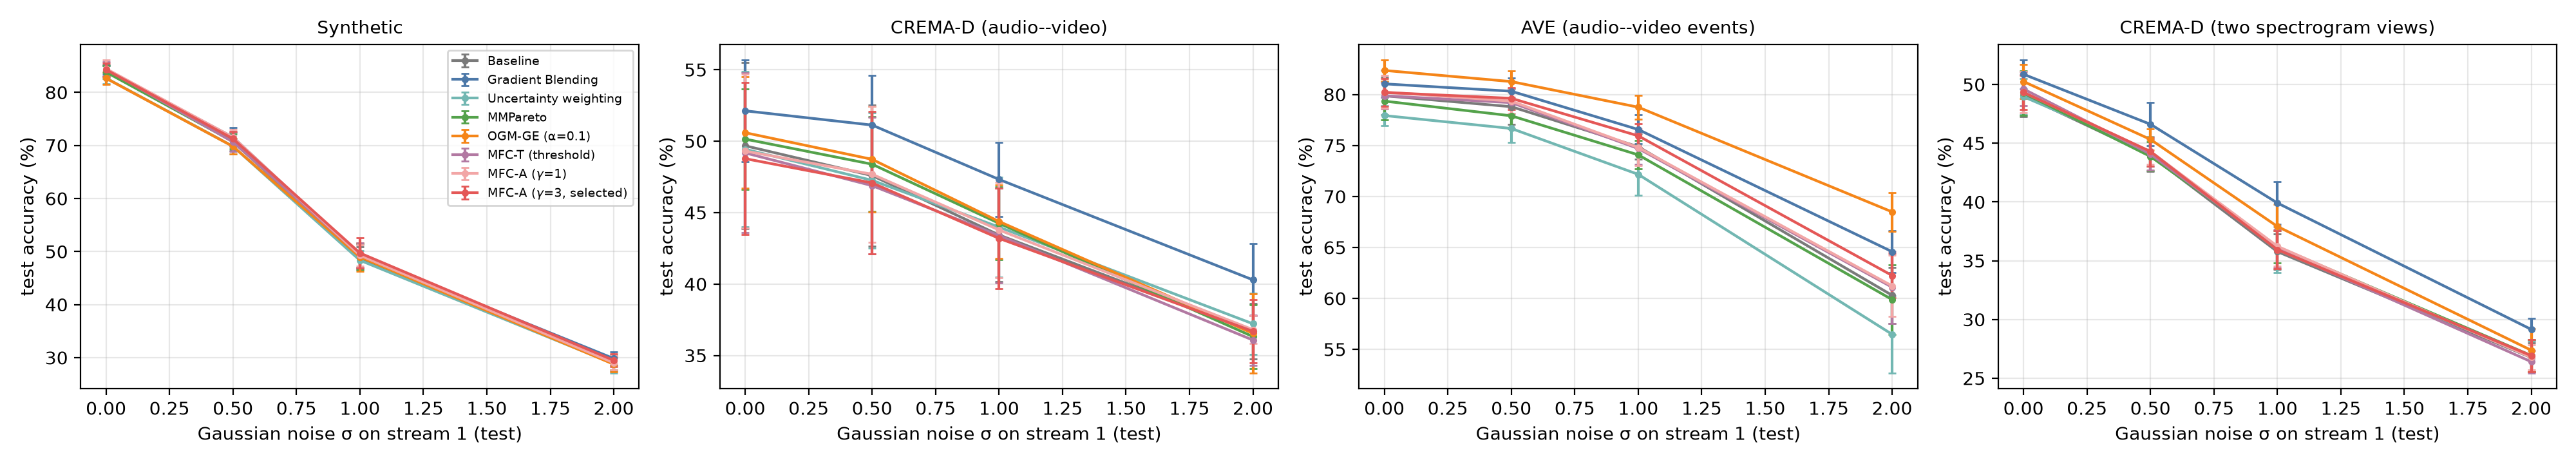
\includegraphics[width=\textwidth]{images/robustness.png}
\caption{\textbf{Robustness to Gaussian noise on the first stream} (test set, mean $\pm$ std over 10 seeds). Panels: synthetic, CREMA-D audio--video, AVE and spectrogram-view control (noise on the first-stream features).}
\label{fig:rob}
\end{figure*}

\subsection*{\DIFadd{Computational cost}}
\DIFadd{Table~\ref{tab:cost} breaks the cost of each method into controller arithmetic, monitoring passes and method-specific work (probe training for Gradient Blending, per-batch gradient processing for OGM-GE and MMPareto). Times are single-thread CPU measurements averaged over ten runs (synthetic runs on a laptop CPU, }\DIFaddend CREMA-D \DIFdelbegin \DIFdel{outcomes support the main argument. The noise injection of }\DIFdelend \DIFaddbegin \DIFadd{runs on a 24-core workstation, so times are comparable within, not across, datasets); FLOPs are computed analytically from the layer sizes. The controller arithmetic of MFC-A is negligible (a few milliseconds and 960 scalar operations per run). The monitoring passes are not negligible in FLOPs, at about 39\% of baseline training FLOPs on both models, because they run inference over the full training split every epoch. In wall-clock time, however, they add only 6.1\% (synthetic) and 18.4\% (audio--video) to the training time, since inference passes are batched and need no backward pass. The running variant removes the training pass and costs 1.8\% and 3.6\% extra time and 7.9\% and 7.5\% extra FLOPs, respectively; its balance is comparable on audio--video but weaker on the synthetic data (Table~\ref{tab:ablation}). Among the baselines, Gradient Blending's probe adds 24--132\% time, MMPareto's per-encoder gradient processing adds 103--168\%, and }\DIFaddend OGM-GE \DIFdelbegin \DIFdel{has very good balance (OGR gap: 5.91)at the cost of the useful gradients of the predominating spatial modality, damaging accuracy by $-3.1\%$. MFC then discovers the Pareto optimum point: matching the Baseline performance (accuracy $+0.18\%$), but narrowing the OGR difference by 38.9\% and increasing robustness at $\sigma{=}1.0$ by $+$2.0\% confirming that the throttle-and-amplify mechanism forces the band-stats encoder to develop genuinely independent discriminative features}\DIFdelend \DIFaddbegin \DIFadd{adds 45--67\% time but only about 1\% FLOPs, because its per-tensor gradient scaling and noise generation are dominated by per-operation overhead rather than arithmetic}\DIFaddend .

\DIFdelbegin %DIFDELCMD < \begin{figure*}[tbp]
%DIFDELCMD <     \centering
%DIFDELCMD <     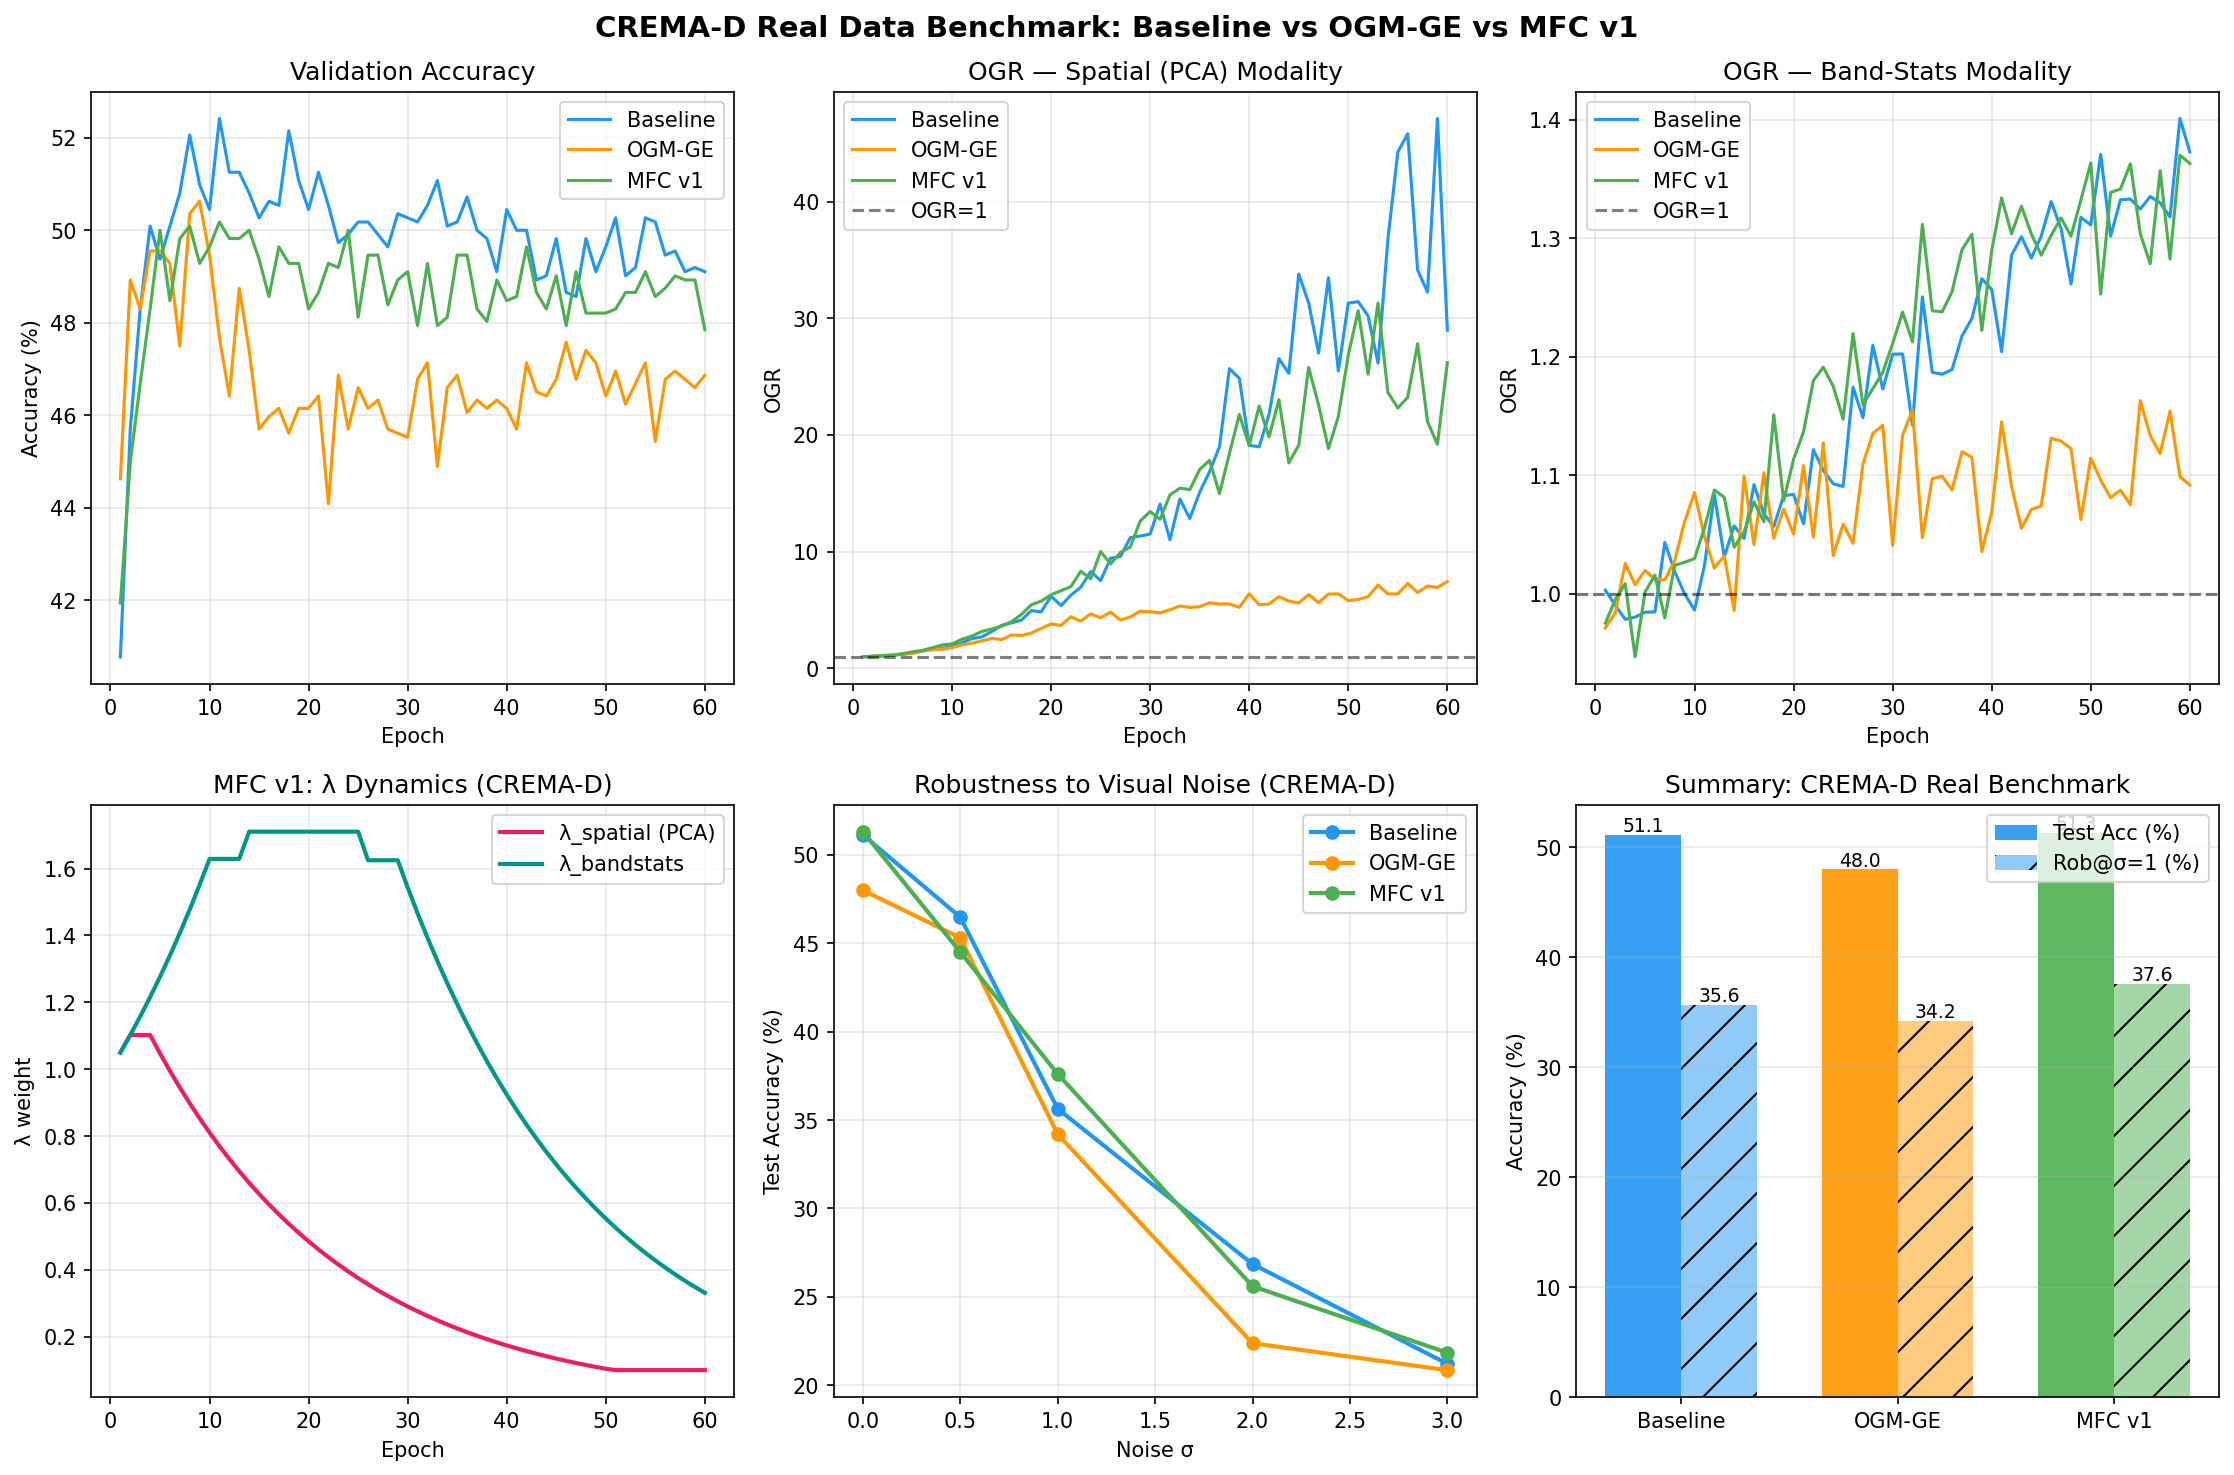
\includegraphics[width=0.85\textwidth]{images/crema_benchmark.png}
%DIFDELCMD <     \caption{\textbf{CREMA-D Benchmark.} Top: validation curves and per-modality OGR trajectories. Bottom: MFC weight dynamics (spatial modality throttled; band-stats amplified), robustness curve, and summary bar chart. Lambda dynamics on real CREMA-D data closely mirror the synthetic benchmark, confirming the OGR signal is a reliable cross-domain modality-imbalance detector.}
%DIFDELCMD <     \label{fig:crema}
%DIFDELCMD < \end{figure*}
%DIFDELCMD < %%%
\DIFdelend \DIFaddbegin \begin{table*}[t]
\caption{\textbf{Cost per training run} (mean over 10 seeds). Ctrl: controller arithmetic time; Monitor: inference passes consumed by the controller; Method: method-specific work; Extra time: (Ctrl+Monitor+Method)/baseline training time; Ctrl ops: scalar operations; Extra FLOPs: (monitor+method FLOPs)/baseline training FLOPs.}
\label{tab:cost}
\centering
\footnotesize
\begin{tabular}{@{}llrrrrrr@{}}
\toprule
\textbf{Data} & \textbf{Method} & \textbf{Ctrl (ms)} & \textbf{Monitor (s)} & \textbf{Method (s)} & \textbf{Extra time (\%)} & \textbf{Ctrl ops} & \textbf{Extra FLOPs (\%)} \\ \midrule
Synthetic & Baseline & 0.0 & 0.00 & 0.00 & 0.0 & 0 & 0.0 \\
Synthetic & Gradient Blending & 0.0 & 0.00 & 1.78 & 131.5 & 0 & 21.6 \\
Synthetic & Uncertainty weighting & 0.0 & 0.00 & 0.00 & 0.0 & 0 & 0.0 \\
Synthetic & MMPareto & 0.3 & 0.00 & 1.40 & 103.0 & 0 & 63.2 \\
Synthetic & OGM-GE & 0.0 & 0.00 & 0.91 & 66.7 & 0 & 1.2 \\
Synthetic & MFC-T & 3.1 & 0.08 & 0.00 & 6.1 & 960 & 39.5 \\
Synthetic & MFC-A (extra train pass) & 3.0 & 0.08 & 0.00 & 6.1 & 960 & 39.5 \\
Synthetic & MFC-A (running loss) & 3.0 & 0.02 & 0.00 & 1.8 & 960 & 7.9 \\
CREMA-D & Baseline & 0.1 & 0.00 & 0.00 & 0.0 & 0 & 0.0 \\
CREMA-D & Gradient Blending & 0.1 & 0.00 & 3.50 & 24.1 & 0 & 16.2 \\
CREMA-D & Uncertainty weighting & 0.2 & 0.00 & 0.00 & 0.0 & 0 & 0.0 \\
CREMA-D & MMPareto & 0.1 & 0.00 & 24.35 & 167.9 & 0 & 63.2 \\
CREMA-D & OGM-GE & 0.1 & 0.00 & 6.53 & 45.1 & 0 & 0.6 \\
CREMA-D & MFC-T & 14.7 & 2.88 & 0.00 & 19.9 & 1280 & 39.1 \\
CREMA-D & MFC-A (extra train pass) & 14.4 & 2.65 & 0.00 & 18.4 & 1280 & 39.1 \\
CREMA-D & MFC-A (running loss) & 12.1 & 0.51 & 0.00 & 3.6 & 1280 & 7.5 \\
\bottomrule
\end{tabular}
\end{table*}
\DIFaddend 

\DIFdelbegin \section{\DIFdel{Discussion}}
%DIFAUXCMD
\addtocounter{section}{-1}%DIFAUXCMD
\subsection{\DIFdel{Complexity Analysis}}
%DIFAUXCMD
\addtocounter{subsection}{-1}%DIFAUXCMD
\DIFdel{In Table \ref{tab:complexity}, we estimate Proposed approach in comparison to standard baselines in terms of asymptotic complexity. The MFC needs a small history buffer of size $H$ (Window size) of each modality. OGR computation is $O(1)$ per epoch. Gradient Blending on the contrary uses $M+1$ models (M the number of modalities) to completely converge and estimate the best weights offline.
}\DIFdelend \DIFaddbegin \section*{\DIFadd{Discussion}}
\paragraph{\DIFadd{What the evidence supports.}} \DIFadd{Across four datasets, MFC-A does what it is designed to do: it detects the stream whose training loss is decoupling from its held-out loss and transfers auxiliary supervision away from it, whether that stream is the more accurate one (AVE) or not (CREMA-D). On AVE and on the synthetic benchmark it meets the goal of reducing imbalance (by 63\% and 41\%) and improving robustness without loss of accuracy, and the effect grows with the capacity of the dominant encoder, which is the regime in which gradient starvation is most damaging. On CREMA-D its effects point in the same direction but are not statistically significant, and its effect on clean accuracy is small everywhere. We consider this a realistic characterisation of a bounded scalar loss-weighting method that leaves the joint loss untouched.
}\DIFaddend 

\DIFdelbegin %DIFDELCMD < \begin{table}[h]
%DIFDELCMD < \caption{\textbf{Computational Complexity Comparison.} $N$: Samples, $E$: Epochs, $M$: Modalities, $H$: History Window. Proposed method maintains the linear time complexity of naive training.}
%DIFDELCMD < \label{tab:complexity}
%DIFDELCMD < \centering
%DIFDELCMD < \begin{tabularx}{\columnwidth}{@{}Xcc@{}}
%DIFDELCMD < \toprule
%DIFDELCMD < \textbf{Algorithm} & \textbf{Time} & \textbf{Space} \\ \midrule
%DIFDELCMD < Naive Joint Training & $O(N \cdot E)$ & $O(\theta)$ \\
%DIFDELCMD < Gradient Blending & $O(N \cdot E \cdot M)$ & $O(\theta \cdot M)$ \\
%DIFDELCMD < OGM-GE & $O(N \cdot E + N \cdot M)$ & $O(\theta)$ \\
%DIFDELCMD < \textbf{MFC (Proposed)} & $O(N \cdot E)$ & $O(\theta + M \cdot H)$ \\ \bottomrule
%DIFDELCMD < \end{tabularx}
%DIFDELCMD < \end{table}
%DIFDELCMD < %%%
\DIFdelend \DIFaddbegin \paragraph{\DIFadd{When to prefer alternatives.}} \DIFadd{No single method was best everywhere. OGM-GE was the strongest on vision-dominant AVE, where directly scaling down the visual encoder's gradients every mini-batch acts more strongly than reweighting auxiliary losses once per epoch, but on the synthetic benchmark its selected setting cost accuracy. Gradient Blending was the strongest on both CREMA-D settings; there its offline estimate pushed almost all auxiliary weight onto one stream ($\lambda_v{=}0$ on audio--video, $0.14$ on the spectrogram views), an extreme allocation that MFC-A's bounded, smoothed law cannot reach. The static-weight ablation suggests that the allocation, rather than its dynamics, drives most of the benefit; MFC-A's advantage is that it finds a direction in one run without a probe, at the price of being conservative. When an extra probe run is affordable, Gradient Blending is a strong choice. OGM-GE can enforce balance more aggressively but trades accuracy for it, and its $\alpha$ must be tuned. MFC-A's advantages are that it runs in a single pass, uses the same smoothing hyper-parameters on every dataset, never reduced accuracy significantly at $p<0.05$ (the largest drop, $-0.9$ points on audio--video, has $p{=}0.05$), and exposes an interpretable signal ($\OGR_m(t)$, $\lambda_m(t)$) that can be monitored even when it is not used for control.
}\DIFaddend 

\DIFdelbegin \subsection{\DIFdel{Qualitative Observations}}
%DIFAUXCMD
\addtocounter{subsection}{-1}%DIFAUXCMD
\DIFdel{During the baseline runs, the Audio OGR is held almost at 1.0 with the Vision OGR jumping to 1.5, which implies that the Audio encoder is virtually learning nothing (there are no gradients) and the Vision encoder is learning a lot (gradients are large). }\DIFdelend \DIFaddbegin \paragraph{\DIFadd{Why a ratio.}} \DIFaddend The \DIFdelbegin \DIFdel{weights $\lambda_a$ of the Audio in the MFC runs steadily increase, however, during the first 10 epochs (The ``Amplify'' rule active)reaching about 3.5, and then levels off.
This effectively recreates the audio gradients and the model must utilize the spectrograms to extract the emotion cues instead of using facial expression in the CIFAR like images. }\DIFdelend \DIFaddbegin \DIFadd{scale-invariance argument (Proposition~\ref{prop:scale}) is the main reason to prefer OGR over the raw gap, and the signal ablation supports it: the raw-gap controller balances less on the two datasets with unequal loss scales and behaves like OGR on the spectrogram control, whose two views have similar loss scales. The differences are modest, however, and only the effect on the weak head's accuracy is significant, so we regard the empirical support as consistent with, rather than proof of, the theoretical argument.
}\DIFaddend 

\DIFdelbegin \subsection{\DIFdel{Limitations and Future Work}}
%DIFAUXCMD
\addtocounter{subsection}{-1}%DIFAUXCMD
\DIFdel{Although promising, Proposed approach is based on the assumption that the separate validation set is a good indicator ofthe generalization ability on the target distribution.
The OGR signal can be misleading in case the validation set is biased. Besides, in the case of foundational models with billions of parameters the ``Generalization Gap'' could not be observed until very late in training , necessitating a special warm-up strategy.
}\DIFdelend \DIFaddbegin \paragraph{\DIFadd{Limitations.}} \DIFadd{(i) MFC-A needs a held-out controller split. We kept it disjoint from both the tuning and the test data, which costs training data; in practice the standard validation set could serve as the controller split if model selection is done on another subset. (ii) Our models operate on fixed features with small MLP encoders; end-to-end training of large backbones, more than two modalities and larger audio--visual corpora (Kinetics-Sounds, VGGSound\mbox{%DIFAUXCMD
\cite{chen2020vggsound}}\hskip0pt%DIFAUXCMD
, AudioSet\mbox{%DIFAUXCMD
\cite{gemmeke2017audio}}\hskip0pt%DIFAUXCMD
) remain to be tested. Combining MFC-A's generalization signal with per-batch gradient modulation of the kind used by OGM-GE is a natural next step. (iii) Baselines are re-implementations in a shared late-fusion setting and may not reproduce the absolute numbers of their original papers; AGM, PMR and OLM were not evaluated. (iv) Only the auxiliary unimodal losses are re-weighted, within fixed bounds; extending the controller to the joint term, to per-encoder learning rates or to attention-level gates, and allowing a modality's auxiliary weight to reach zero, is future work. (v) The pixel-level degradations are synthetic; generative adverse-condition data such as rain and night images\mbox{%DIFAUXCMD
\cite{lan2025sustechgan} }\hskip0pt%DIFAUXCMD
would provide a more realistic test. (vi) $\gamma$ is selected from three values per dataset; although the rule uses no test data, a larger candidate set would increase the risk of overfitting the tuning split.
}\DIFaddend 

\DIFdelbegin \DIFdel{Future research will be concerned with:
}%DIFDELCMD < \begin{itemize}
\begin{itemize}%DIFAUXCMD
%DIFDELCMD <     \item %%%
\item%DIFAUXCMD
\textbf{\DIFdel{High-Resolution Regimes}}%DIFAUXCMD
\DIFdel{: ImageNet + AudioSet\mbox{%DIFAUXCMD
\cite{gemmeke2017audio}}\hskip0pt%DIFAUXCMD
validation of MFC. }%DIFDELCMD < \item %%%
\item%DIFAUXCMD
\textbf{\DIFdel{Transformer Integration}}%DIFAUXCMD
\DIFdel{: Using MFC on attention head dropout rates in place of global loss weights. }%DIFDELCMD < \item %%%
\item%DIFAUXCMD
\textbf{\DIFdel{Real-Time Adaptation}}%DIFAUXCMD
\DIFdel{: MFC can be applied in online learning contexts where the sets of data to be validated are not fixed. }
\end{itemize}%DIFAUXCMD
%DIFDELCMD < \end{itemize}
%DIFDELCMD < 

%DIFDELCMD < %%%
\section{\DIFdel{Conclusion}}
%DIFAUXCMD
\addtocounter{section}{-1}%DIFAUXCMD
\DIFdel{In this paper, we presented a lightweight solution to the Gradient Starvation problem, the Modality Fairness Controller (MFC), a smart, lightweight solution. The MFC also avoids one modality bullying the rest in the process of training by closely monitoring the }\DIFdelend \DIFaddbegin \section*{\DIFadd{Conclusion}}
\DIFadd{We introduced the }\DIFaddend Overfitting-to-Generalization Ratio \DIFdelbegin \DIFdel{(OGR). It achieves this without pre-training or random noise injection which is costly.
}%DIFDELCMD < 

%DIFDELCMD < %%%
\DIFdel{This method is proven by Proposed experiments with the synthetic benchmark and real world CREMA-D corpus. MFC at $\sigma{=}1.0$ - modality imbalance gap is reduced by 38.4\% and visual noise robustness is enhanced by $+4.7\%$ at $\sigma{=}0.5$ and $+2.3\%$ at $\sigma{=}1.0$ }\DIFdelend \DIFaddbegin \DIFadd{as a scale-invariant per-modality diagnostic and MFC-A as a threshold-free, closed-loop controller that uses it to redistribute auxiliary loss weight during a single training run. Under a protocol with ten paired seeds, disjoint controller, tuning and test data, and five baselines, MFC-A maintained accuracy on every dataset. On the real AVE benchmark it reduced the OGR-measured imbalance by 63\% and significantly improved robustness to noise, blur and low light; }\DIFaddend on the synthetic benchmark \DIFdelbegin \DIFdel{. On actual }\DIFdelend \DIFaddbegin \DIFadd{it reduced the imbalance by 41\%, and by up to 55\% for high-capacity dominant encoders. On }\DIFaddend CREMA-D \DIFdelbegin \DIFdel{data, MFC is more accurate by $+3.1\%$ percent over }\DIFdelend \DIFaddbegin \DIFadd{it identified the overfitting modality correctly, but its improvements were not significant. }\DIFaddend OGM-GE \DIFdelbegin \DIFdel{yet the reduction of the OGR gap is 38.9\% with no noise injection. More to the point, the system is predictable: it works as a thermostat, which cools the overheated modalities and heats the cold ones. Scaling analysis shows the benefit grows with model capacity, from $+0.7\%$ at 128-dim to $+3.1\%$ at 1024-dim, making MFC-A most valuable in large-model regimes}\DIFdelend \DIFaddbegin \DIFadd{(on AVE) and Gradient Blending (on CREMA-D) achieved larger gains at the cost of a tuned hyper-parameter or an extra probe run. Because the controller arithmetic is negligible, the cost of the method lies in its monitoring passes, which a running-loss variant largely removes. We release code, per-epoch logs and data-preparation scripts so that every number in this paper can be regenerated}\DIFaddend .

\section*{Declarations}
\DIFdelbegin %DIFDELCMD < \begin{itemize}
%DIFDELCMD < \item %%%
\DIFdel{Clinical Trial: Not applicable.
}%DIFDELCMD < \item %%%
\DIFdel{Ethics Approval: Not applicable.
}%DIFDELCMD < \item %%%
\DIFdel{Consent to Participate: Not applicable.
}%DIFDELCMD < \item %%%
\DIFdel{Consent to Publish: Not applicable.
}%DIFDELCMD < \item %%%
\DIFdel{Funding: The }\DIFdelend \DIFaddbegin \textbf{\DIFadd{Clinical trial, ethics approval, consent to participate and consent to publish:}} \DIFadd{not applicable; the study uses only publicly released datasets and collected no new data from human participants. }\textbf{\DIFadd{Funding:}} \DIFadd{the }\DIFaddend authors received no financial support from any organization for the submitted work. \DIFdelbegin %DIFDELCMD < \item %%%
\DIFdel{Conflict of Interest: The }\DIFdelend \DIFaddbegin \textbf{\DIFadd{Conflict of interest:}} \DIFadd{the }\DIFaddend authors declare that they have no conflict of interest relevant to the content of this article. \DIFdelbegin %DIFDELCMD < \item %%%
\DIFdel{Data Availability: The }\DIFdelend \DIFaddbegin \textbf{\DIFadd{Data availability:}} \DIFadd{the }\DIFaddend datasets used in this study are publicly available and \DIFdelbegin \DIFdel{properly cited within }\DIFdelend \DIFaddbegin \DIFadd{cited in }\DIFaddend the manuscript. \DIFdelbegin \DIFdel{The experimental analysis was conducted using the CIFAR dataset introduced by Krizhevsky and Hinton for tiny image classification tasks, available at: https://www.cs.toronto.edu/~kriz/cifar.html. Additionally, the }\DIFdelend CREMA-D (Crowd-sourced Emotional Multimodal Actors Dataset)\DIFdelbegin \DIFdel{used for emotion recognition analysis is publicly accessible at : https://github. com/CheyneyComputerScience/CREMA-D and https://www. kaggle.com/datasets/ejlok1/cremad.
}%DIFDELCMD < \item %%%
\DIFdel{Author Contributions: }\DIFdelend \DIFaddbegin \DIFadd{\mbox{%DIFAUXCMD
\cite{cao2014crema} }\hskip0pt%DIFAUXCMD
is available at }\url{https://github.com/CheyneyComputerScience/CREMA-D}\DIFadd{, and the AVE (Audio-Visual Event) dataset\mbox{%DIFAUXCMD
\cite{tian2018audio} }\hskip0pt%DIFAUXCMD
at }\url{https://github.com/YapengTian/AVE-ECCV18}\DIFadd{. }\textbf{\DIFadd{Code availability:}} \DIFadd{the complete code (feature extraction, benchmark and aggregation), the generated synthetic data, the extracted features, the exact split definitions and the per-epoch logs of every run reported in this paper are held in a version-controlled repository that is available to the editor and reviewers on request and will be made public upon acceptance. }\textbf{\DIFadd{Author contributions:}} \DIFaddend Lakshya conducted the experiments and implemented the proposed methodology. A.\DIFdelbegin \DIFdel{K.}\DIFdelend \DIFaddbegin \DIFadd{~K.~}\DIFaddend Bairwa contributed to the conceptualization, methodological design and validation of the results. V.\DIFaddbegin \DIFadd{~}\DIFaddend Tiwari supervised the research and contributed to manuscript writing, critical review and final approval.
\DIFdelbegin %DIFDELCMD < \end{itemize}
%DIFDELCMD < %%%
\DIFdelend 

\DIFdelbegin %DIFDELCMD < \bibliography{references}
%DIFDELCMD < %%%
\DIFdelend \DIFaddbegin \bibliography{references}
\DIFaddend 



\end{document}
